%!TEX root = main.tex
\chapter{Result}\label{chapter:Result}
In this chapter the results of our approach for pose estimation are represented and analyzed. The results are obtained by the new feature-based pose optimization which was developed in Ubitrack Framework. The ground truth data is a sequence video that is provided by the ARTrack. The scene consists of a marker with id 0272 and size 18 cm and some artificial objects to provide more feature points. The video frames involve three difference types of transformations such as rotation, translation and zoom. The ground truth data contains 1034 RGB image frames, two log files that illustrate the pose of camera relative to marker and the pose of marker relative to camera that are tracked by the ARTrack camera precisely. The \autoref{fig:sample_dataset_marker} shows some sample images of our ground truth data set.

\begin{figure}[H]
\centering
\begin{tabular}{cc}
  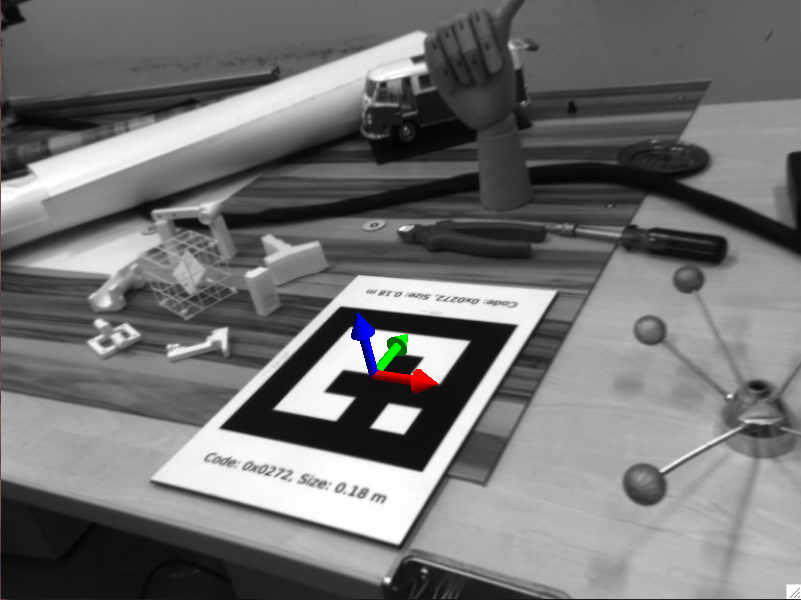
\includegraphics[width=65mm]{figures/sample_0} &   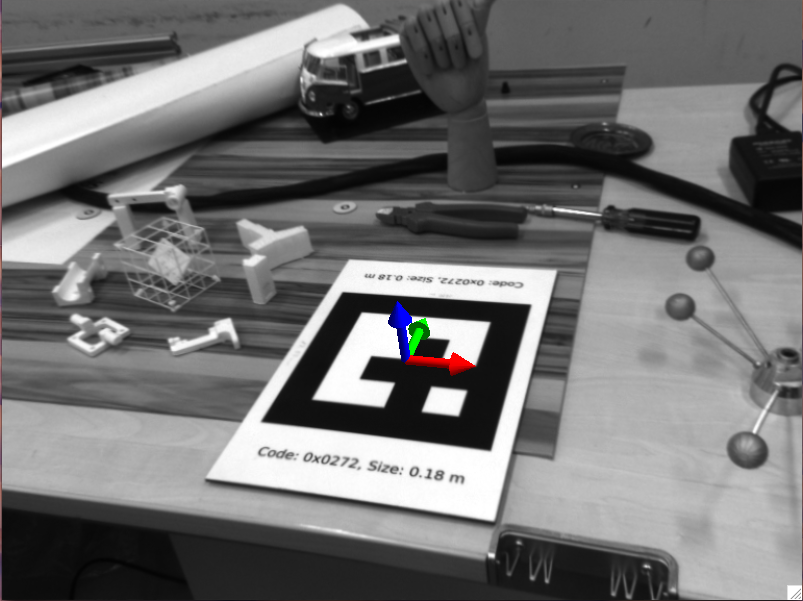
\includegraphics[width=65mm]{figures/sample_1}  \\
  a & b \\[6pt]
  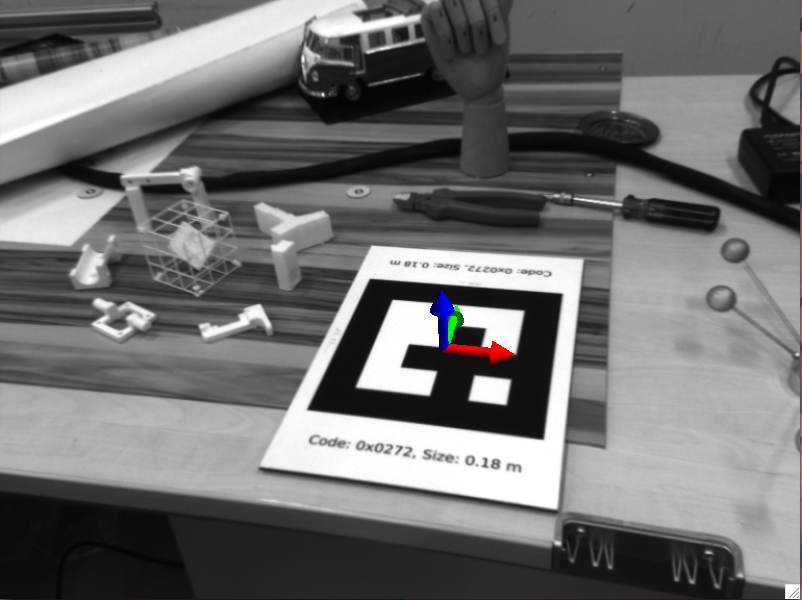
\includegraphics[width=65mm]{figures/sample_2} &   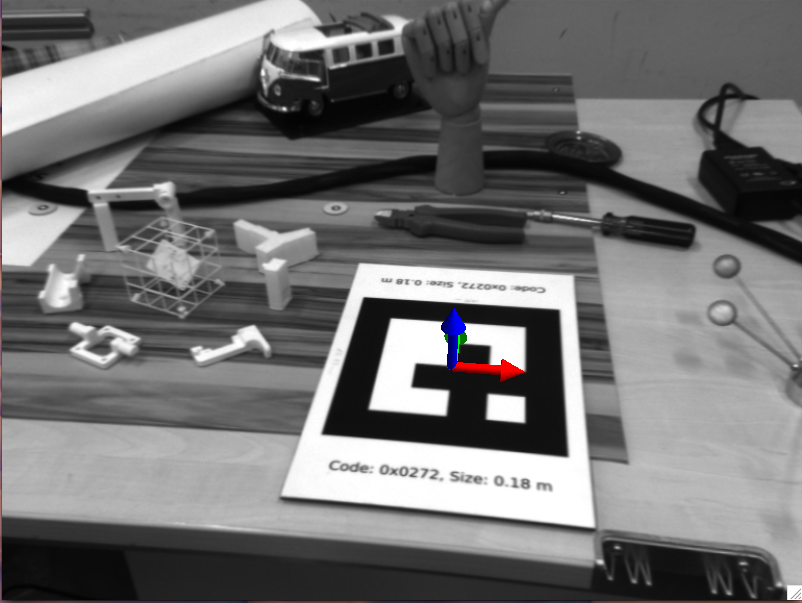
\includegraphics[width=65mm]{figures/sample_3} \\
  c & d \\[6pt]
  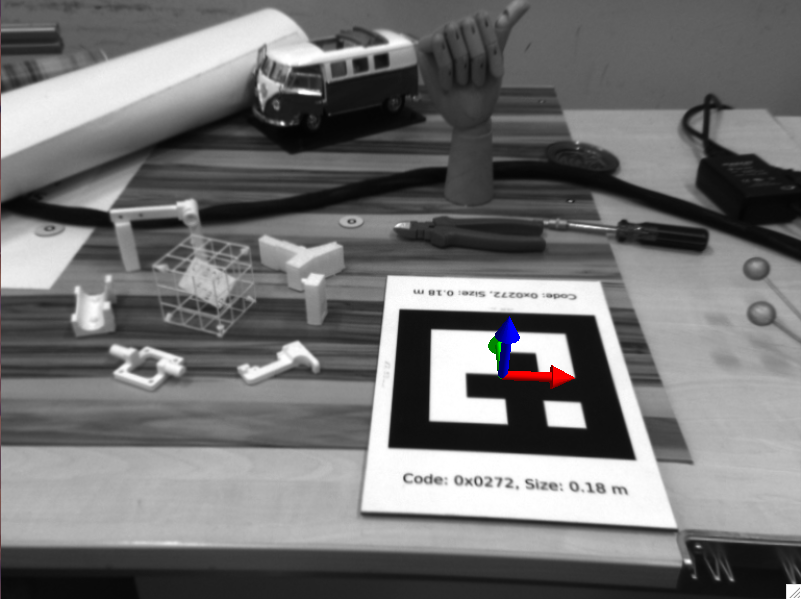
\includegraphics[width=65mm]{figures/sample_4} &   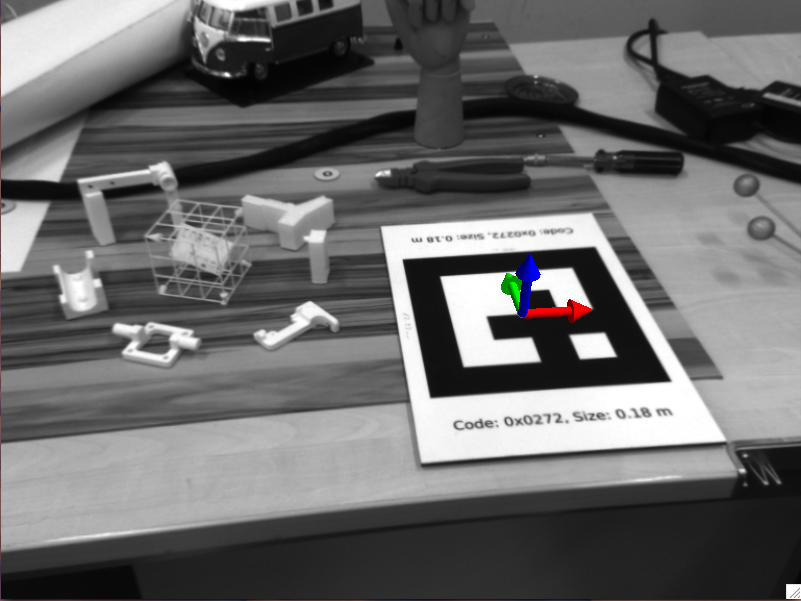
\includegraphics[width=65mm]{figures/sample_5} \\
  e & f \\[6pt]
\end{tabular}
\caption{The sample images of our ground truth data set}\label{fig:sample_dataset_marker}
\end{figure}

In this chapter, the obtained results are analyzed in several aspects. At first, because the size of ground truth data is very big, three sets of 80 sequential images are selected randomly from our ground truth data set. For all sets, the camera has the vertical and horizontal translation, rotation, zoom in and zoom out. \\
In the first test, we analyze the result of each sample data set individually. For each sample data set, the translation errors between the feature-based and ground truth data sample are compared with the error between the marker-based and the same ground truth data. The errors of rotation (in quaternion degree) are also computed for both cases. furthermore, for each data set, an evaluation test is applied that shows the difference between the feature-based and marker-based approaches. We find the translation and rotation between each sequential pair of images (for both methods) and then we compute the distance between these two methods. 

This evaluation test demonstrates the difference between these two methods independent of other parameters that might have effect on our result such as the initial estimated pose that are taken from reference system. For instance, the translation between the first and the second frames which is computed by the markerless approach is compared to the translation between the same frames but for the marker-based approach. The distance between this two approaches is computed by the euclidean distance.\\
% TODO: reason of that 
As it was mentioned in \autoref{chapter:pose_estimation}, we introduced two threshold parameters which define the size of a bundle and the number of frames that are involved for updating the 3D world map and global bundle adjustment. They are called local threshold and global threshold respectively. for the first data sample, the performance of the proposed feature-based approach is evaluated for different values of local and global threshold.\\
Finally, for the first data sample, the performance of the proposed feature-based approach is evaluated based on different methods for initial pose estimation as explained in \autoref{subsec:pose_first_bundle}.

\section{Sample Data Set 1} \label{sec:sample_01}
This set consists of 80 sequential images that cover all three types of movement and transformations (horizontal and vertical movement, rotation and zooming). in feature-based case, we assume that the reference pose for the first bundle are provided by the reference system.

\begin{figure}[H]
\begin{tabular}{cc}
  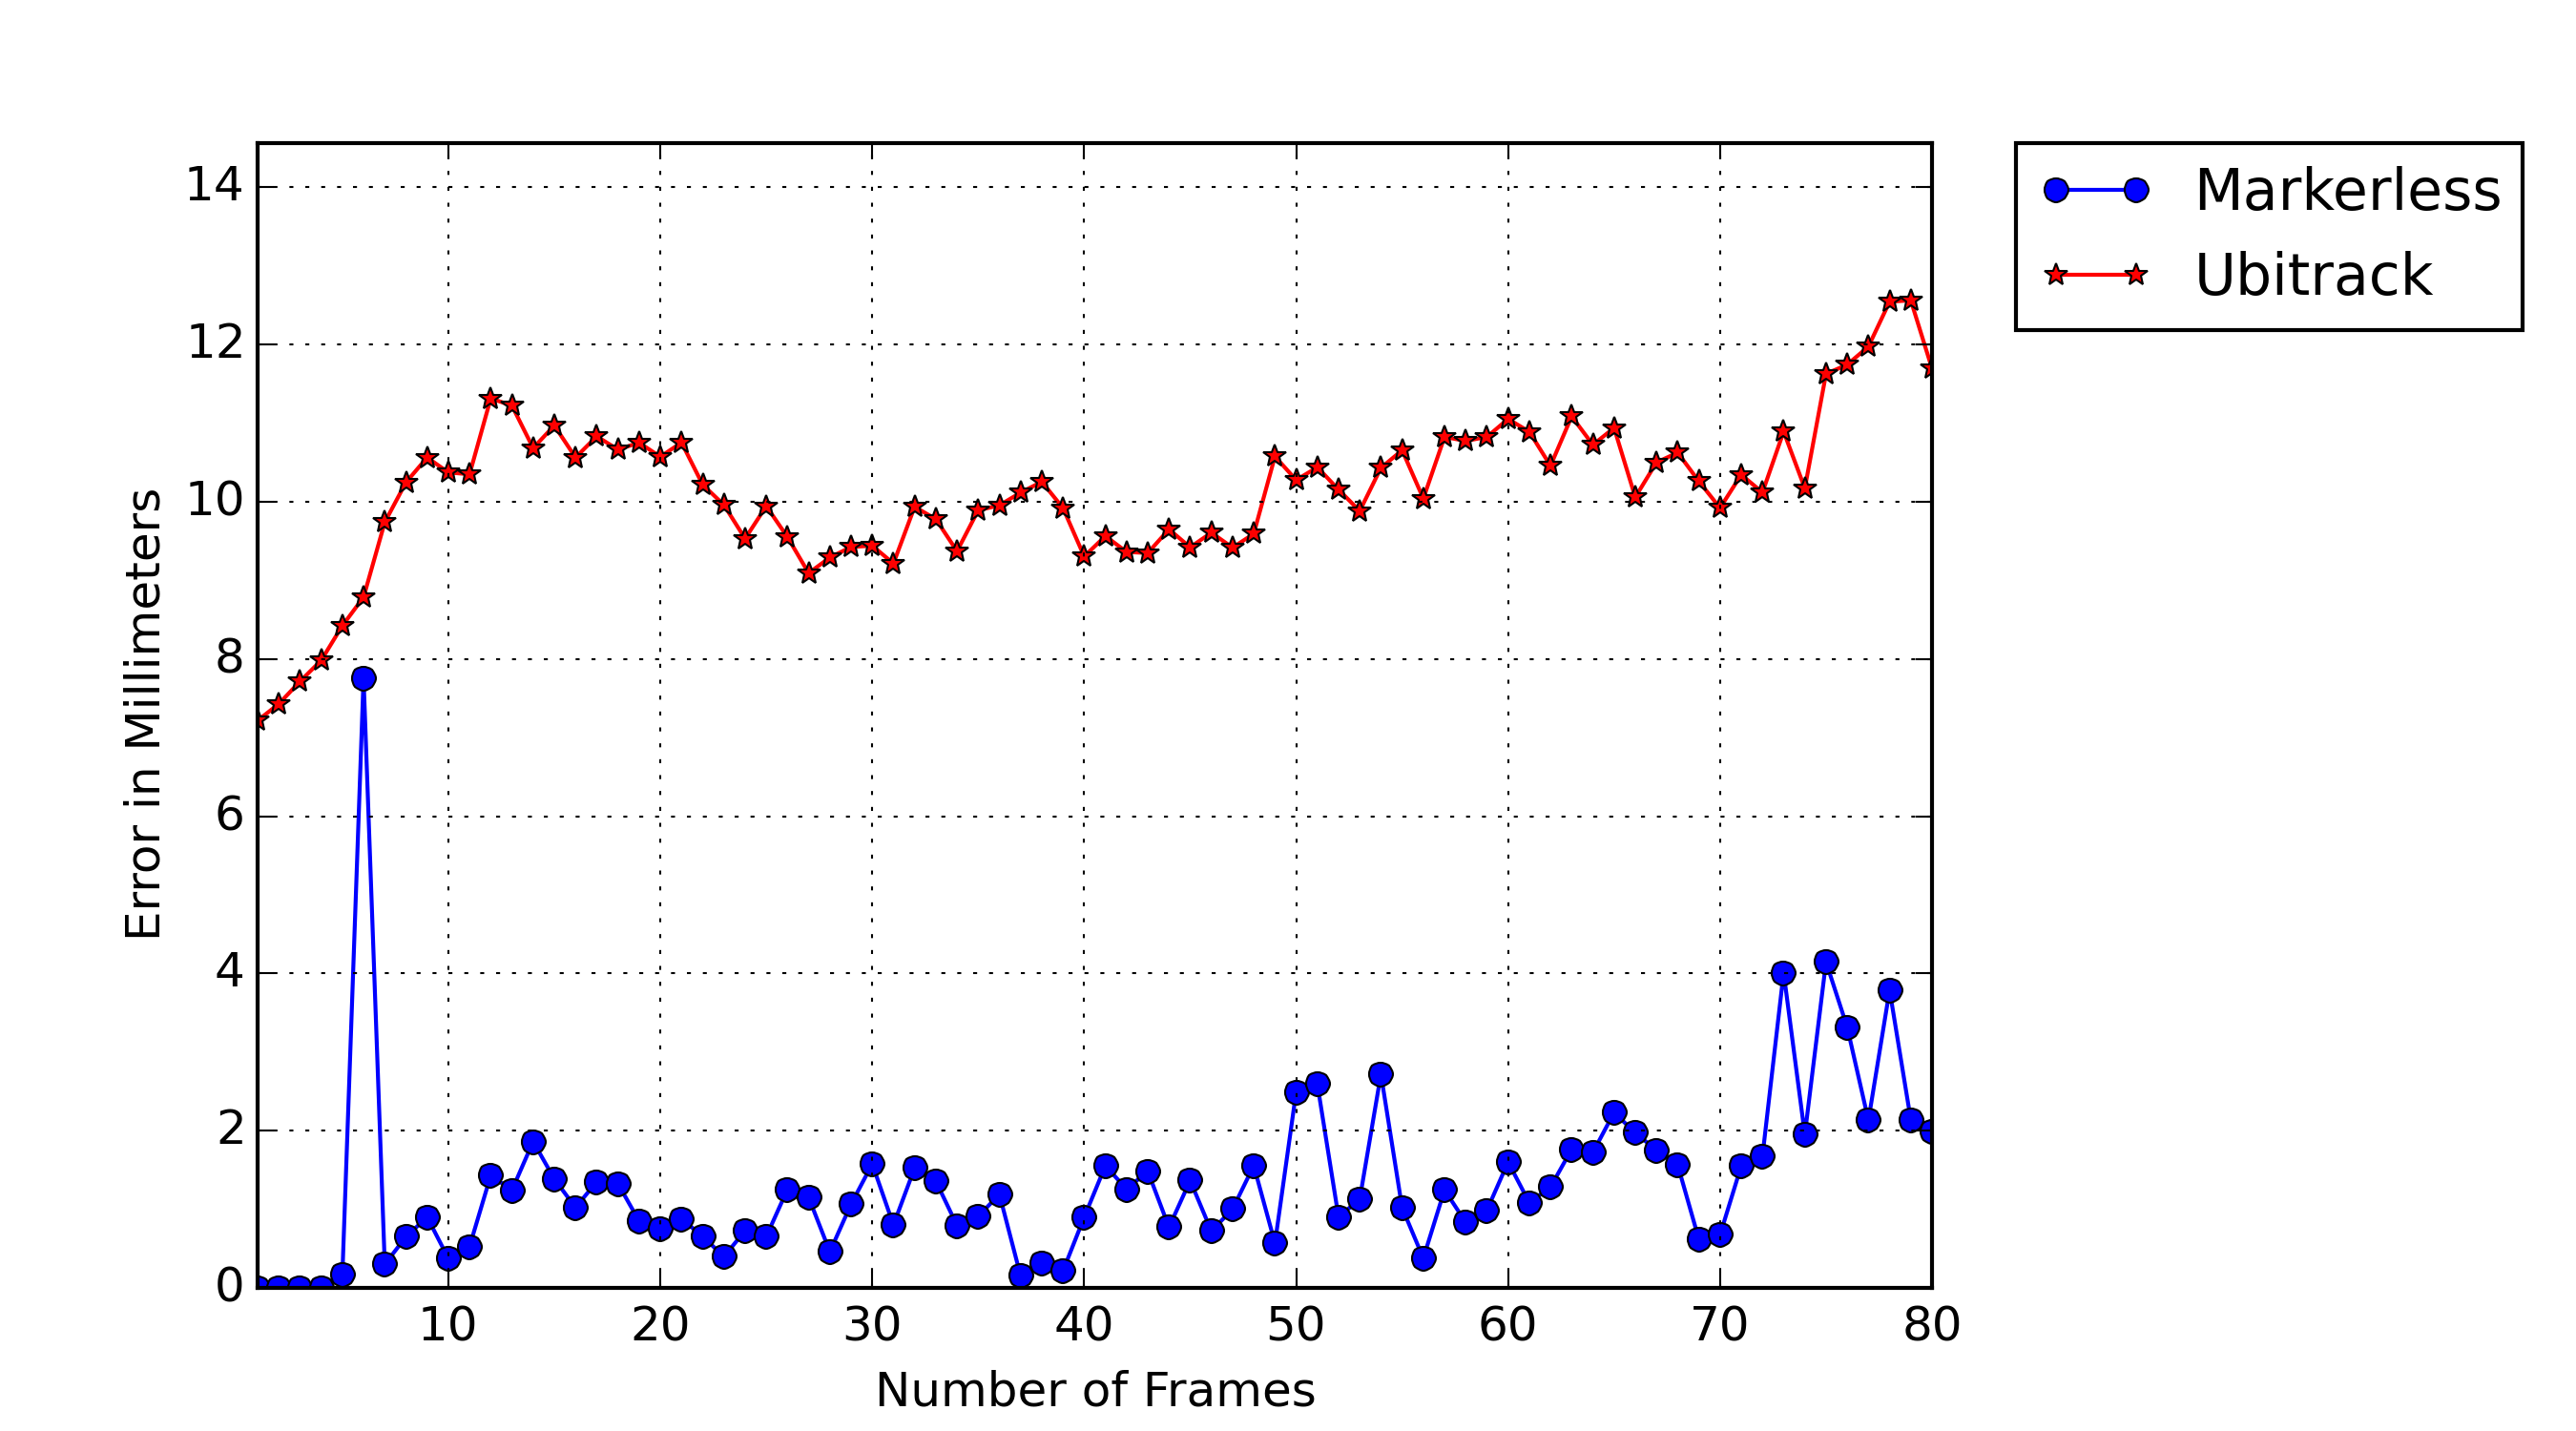
\includegraphics[width=80mm]{figures/global_35/graph_translation} &  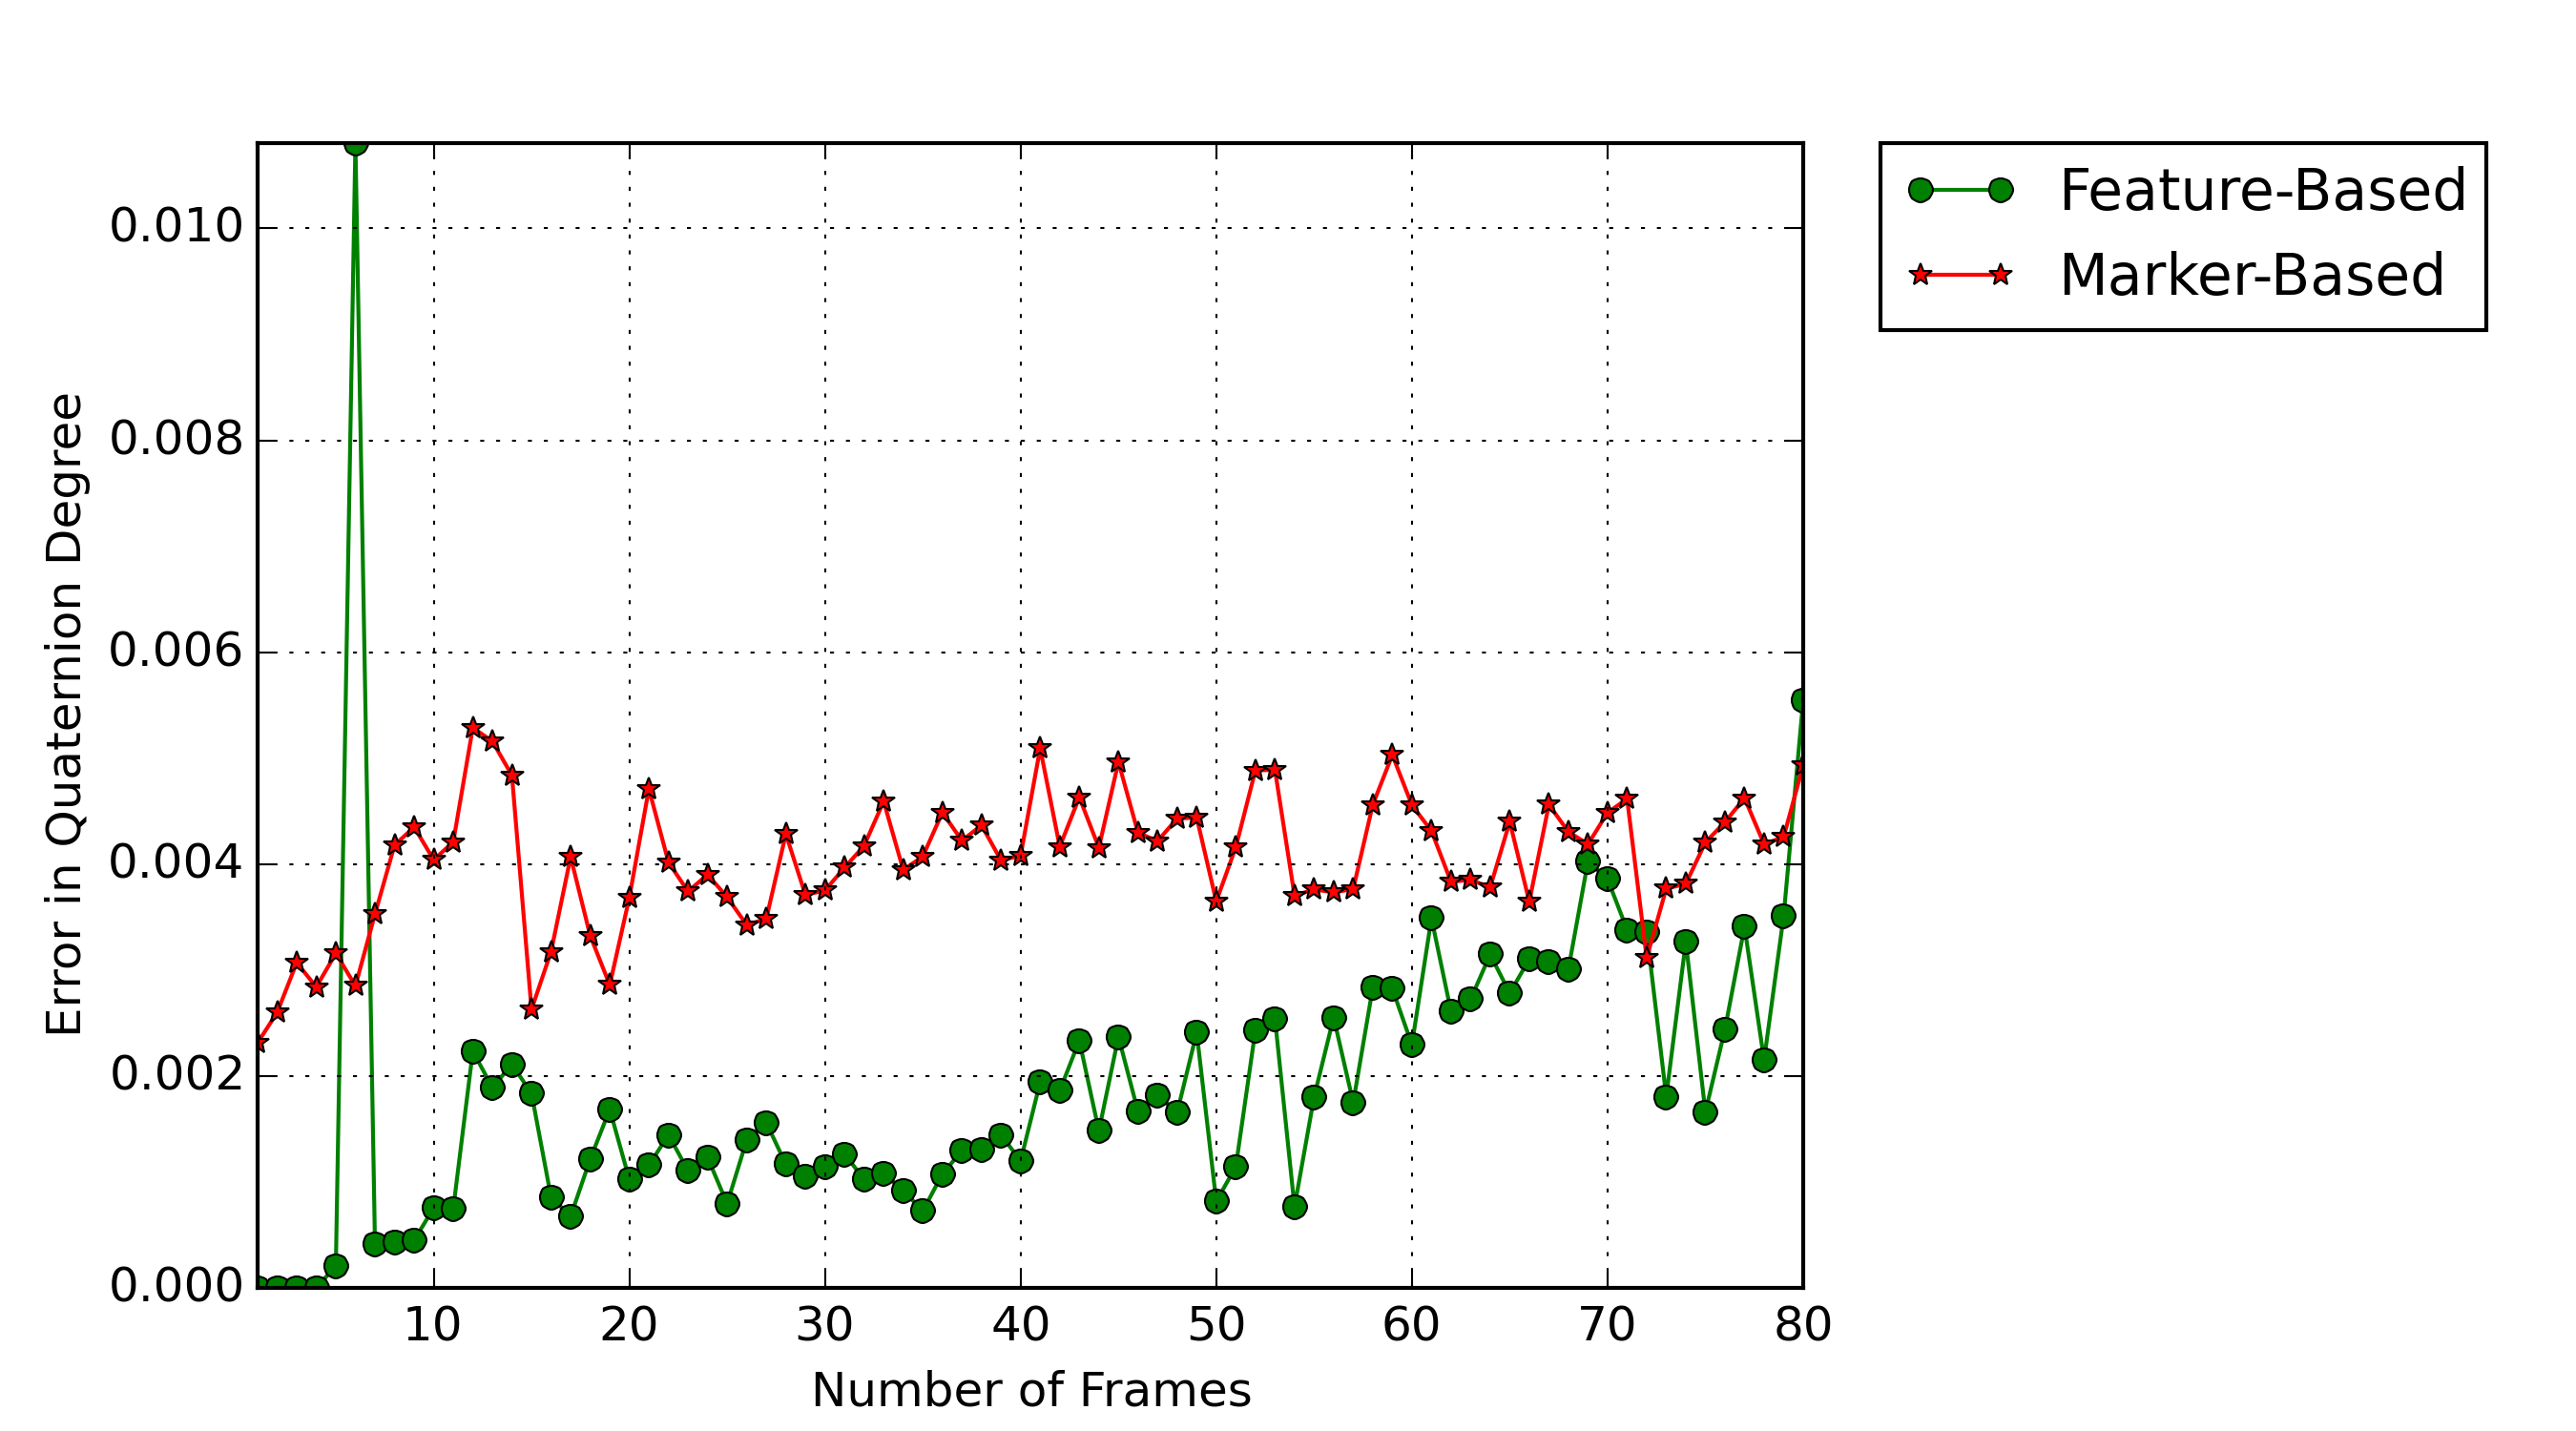
\includegraphics[width=80mm]{figures/global_35/graph_rotation} \\
(a) the translation error in millimeters & (b) the rotation error in quaternion degree \\[6pt]
\end{tabular}
\caption{The tracking errors for both feature-based and marker-based techniques based on the first ground truth data set}   \label{fig:sample_01}
\end{figure}

\begin{table}[H]
\centering
  \begin{tabular}{| c || c | c | c | c |}
      \hline
      & \multicolumn{2}{c|}{Translation} & \multicolumn{2}{c|}{Rotation} \\ \hline
       & Mean & Standard Deviation & Mean & Standard Deviation \\ \hline
      Feature-Based Approach & 1.3303 & 1.1184 & 0.0019 & 0.0015 \\ \hline
      Marker-Base Approach & 10.1552 & 0.9700 & 0.0040 & 0.0006 \\ \hline
  \end{tabular}
  \caption{the statistical analysis of tracking error for both feature-based and marker-based techniques based on the first ground truth data set} \label{tab:sample_01}
\end{table}

Based on both \autoref{fig:sample_01} and \autoref{tab:sample_01}, the tracking result of feature-based is significantly better than marker-based approach for both mean and standard deviation cases. In the case of rotation, the result of marker-less tracking is stable around the 0.0040 degree of quaternion whereas the rotation of feature-based is stable at first but it has a slow increase after the 60th frames. The peak in \autoref{fig:sample_01} (a) and (b) for the 7th image, are the consequence of image blurring. 

\begin{figure}[H]
\begin{tabular}{cc}
  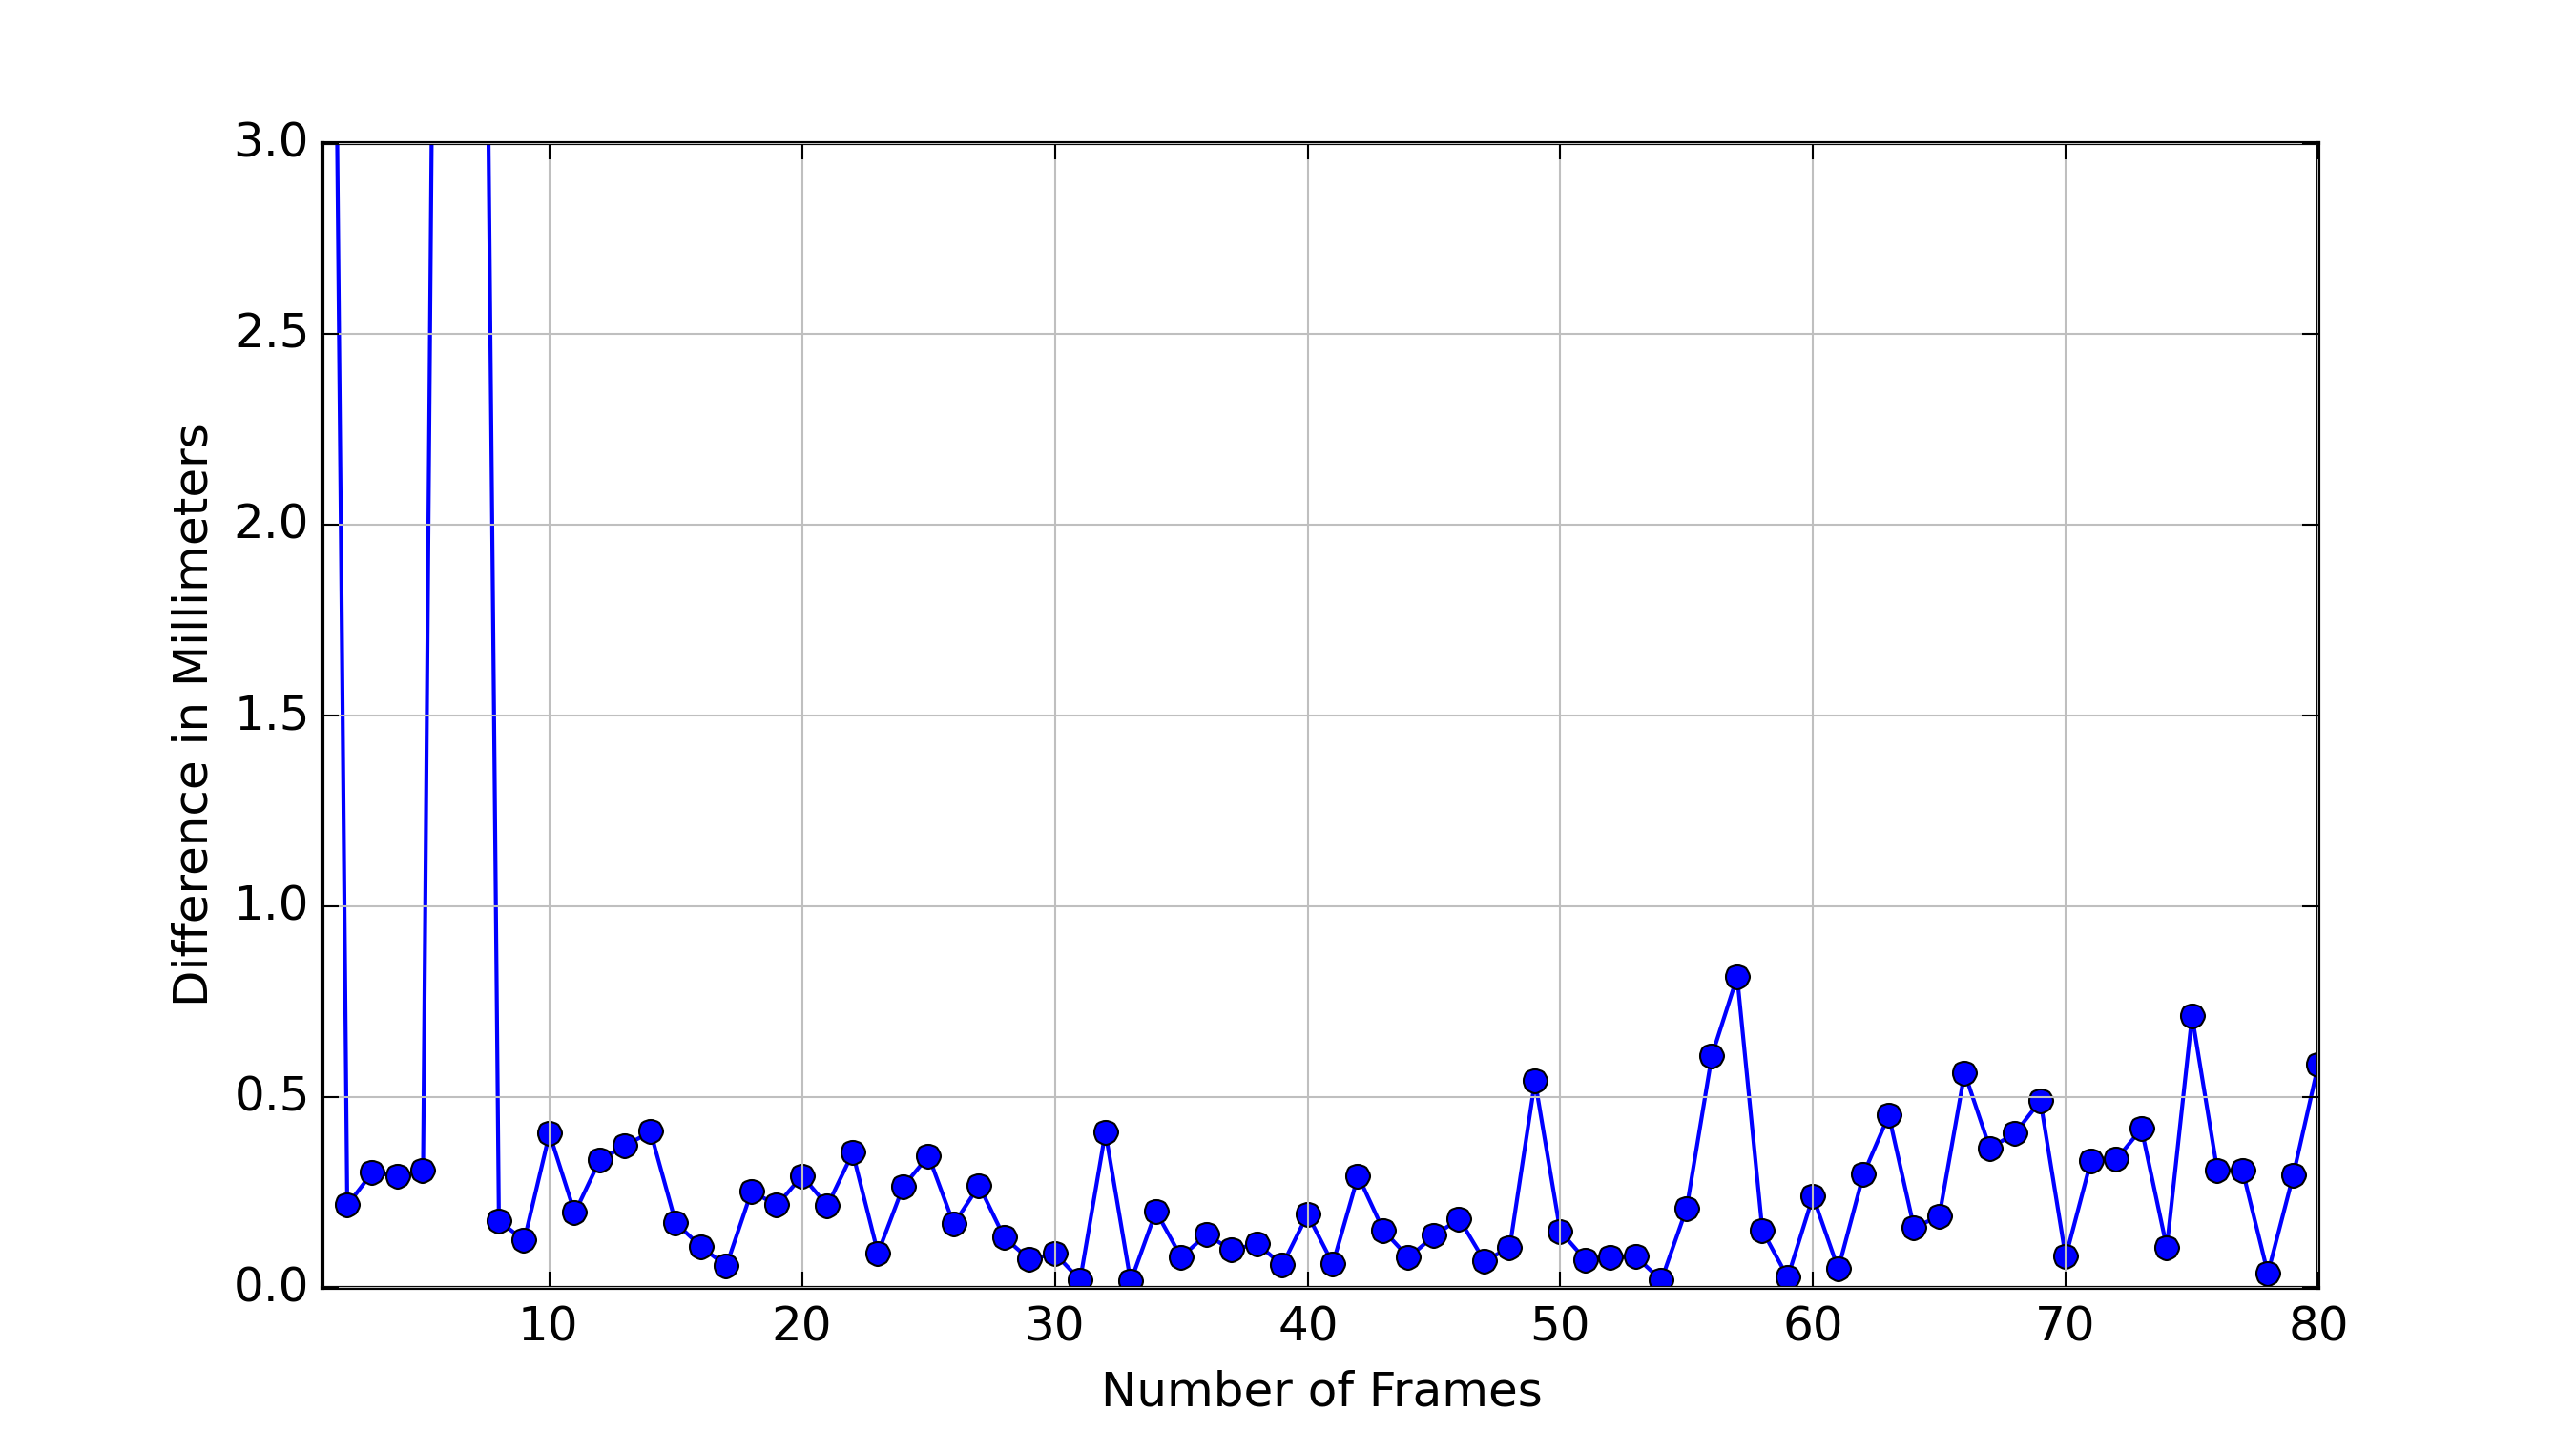
\includegraphics[width=80mm]{figures/diff_0/graph_translation} &  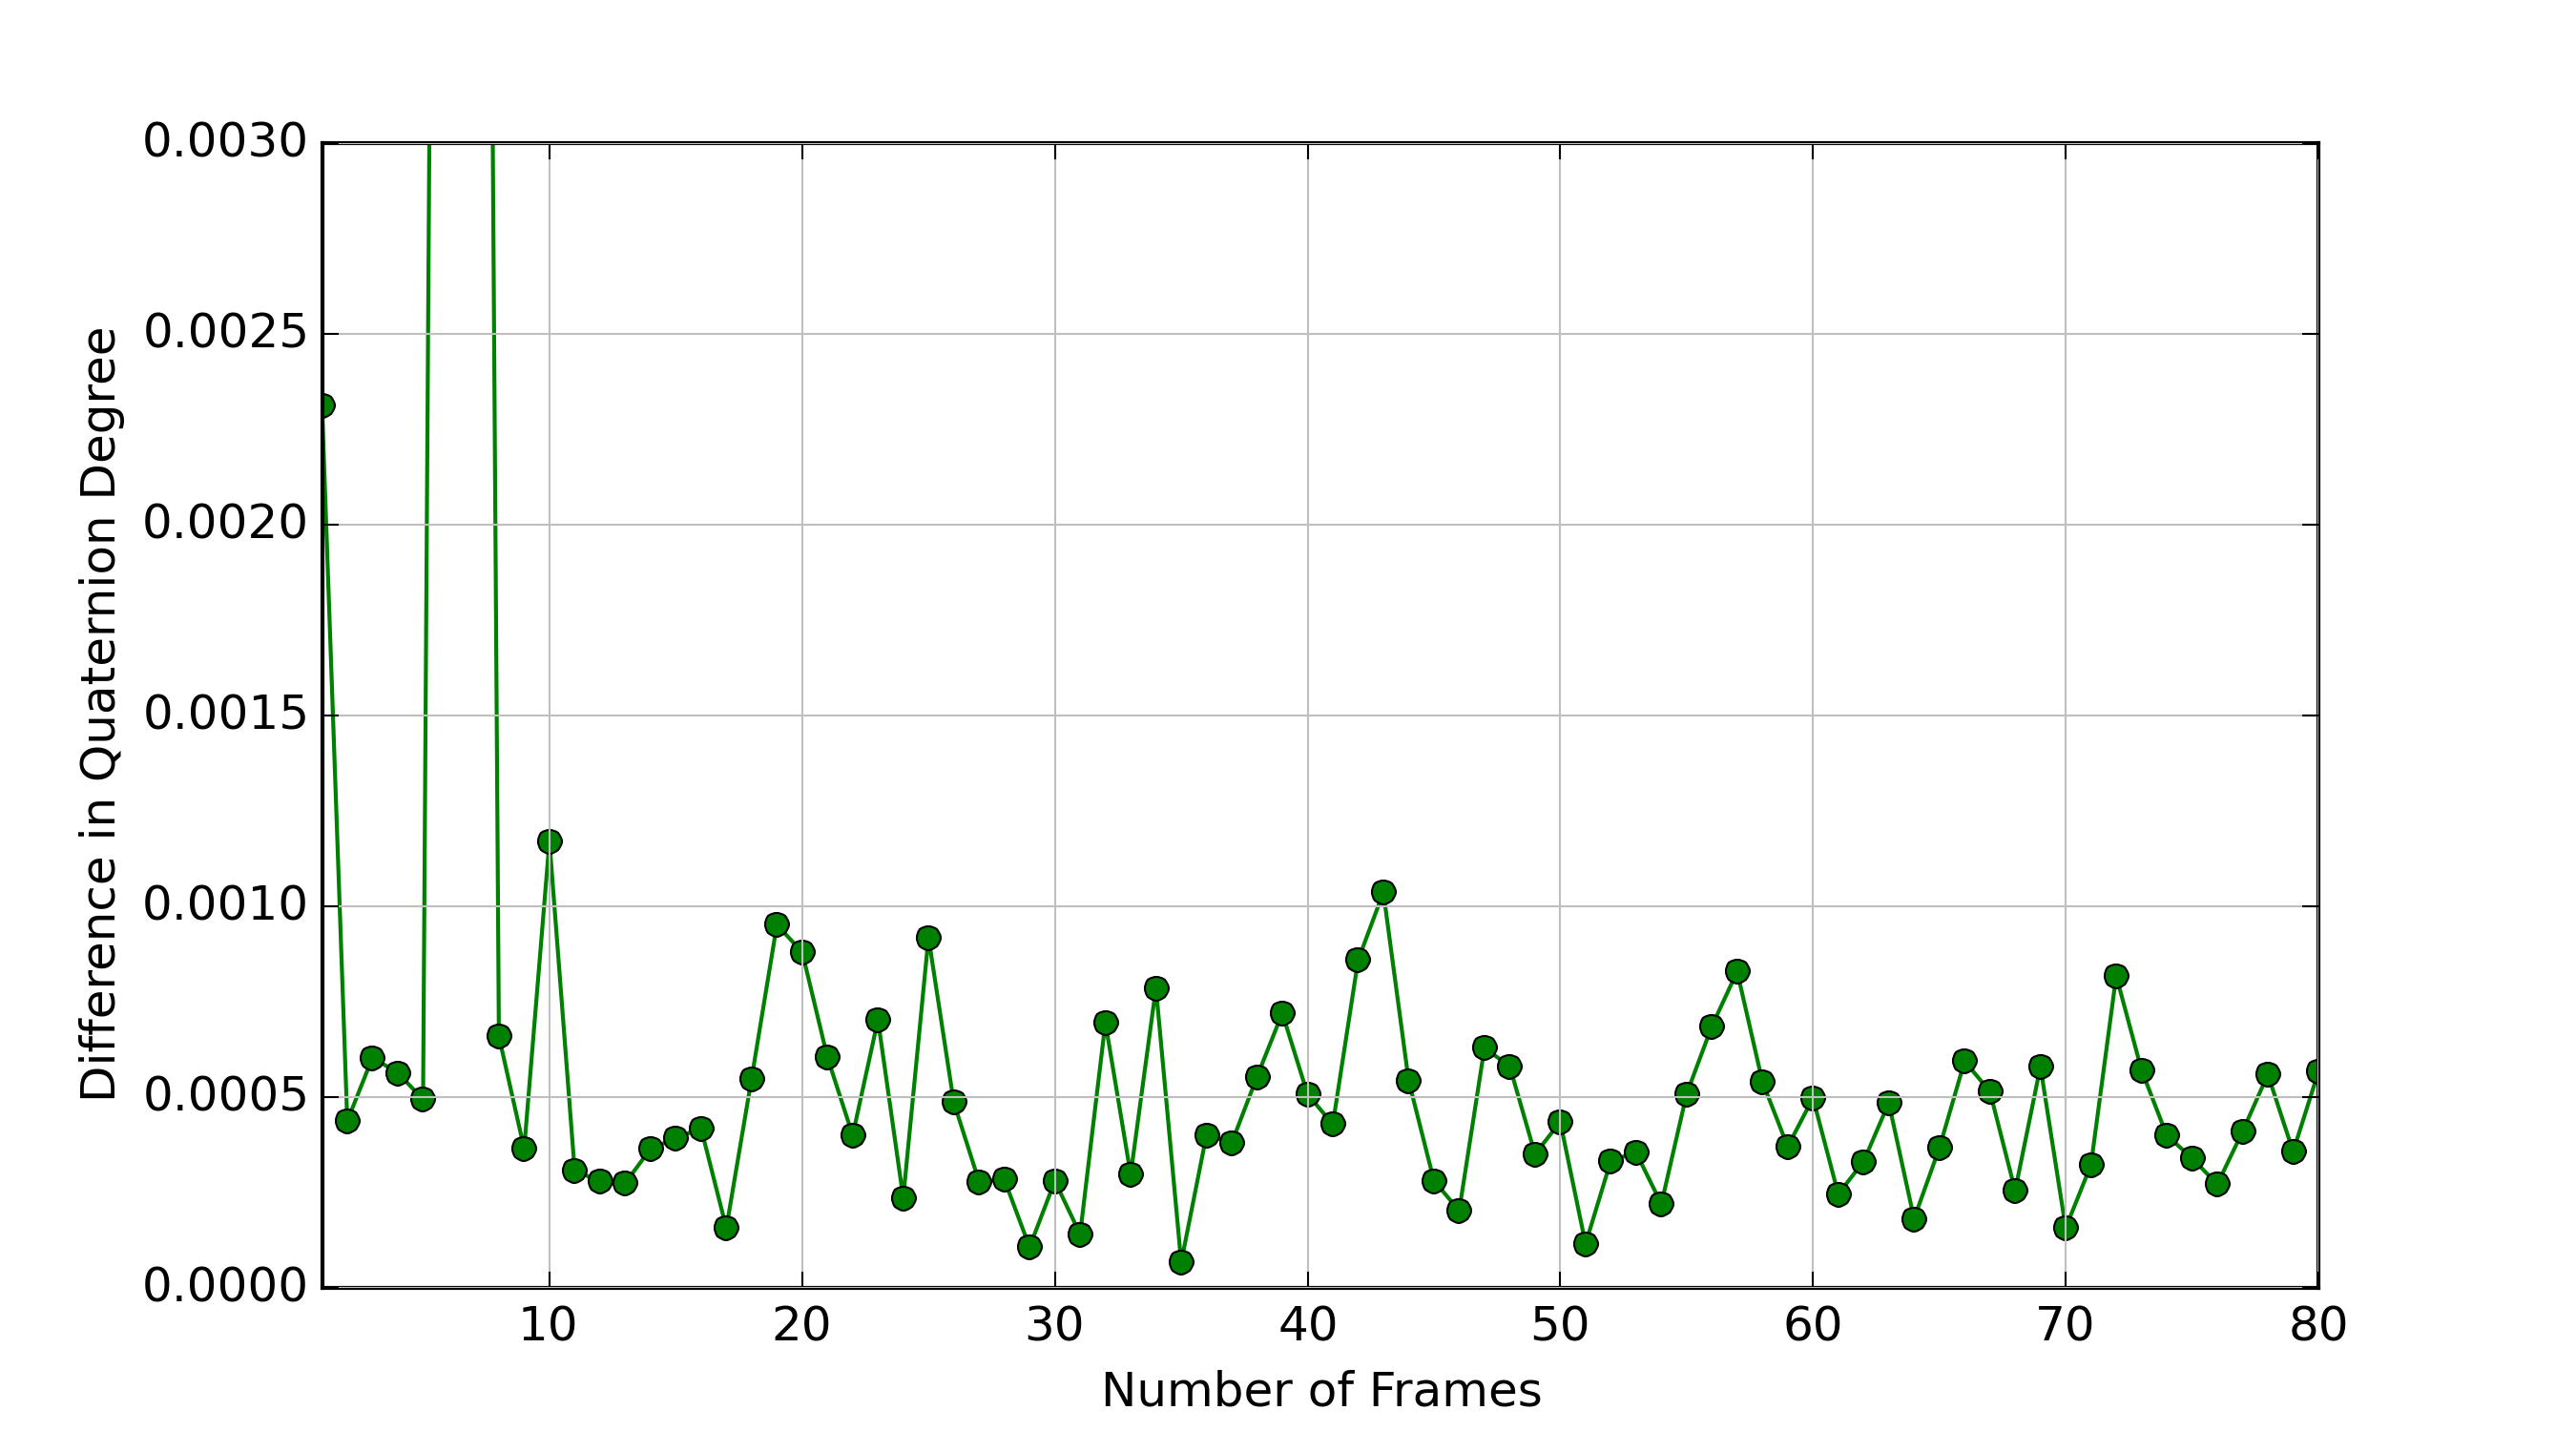
\includegraphics[width=80mm]{figures/diff_0/graph_rotation} \\
(a) difference of translation in milliliters & (b) difference of rotation in degree of quaternion \\[6pt]
\end{tabular}
\caption{The difference between the Feature-based and Marker-based for each sequence pair of first sample data set}\label{fig:sample_01_diff}
\end{figure}

\begin{table}[H]
\centering
  \begin{tabular}{| c | c | c | c |}
      \hline
      \multicolumn{2}{|c|}{Translation} & \multicolumn{2}{c|}{Rotation} \\ \hline
       Mean & Standard Deviation & Mean & Standard Deviation \\ \hline
      0.5089 & 1.3985 & 0.0007 & 0.0016 \\ \hline
  \end{tabular}
  \caption{} \label{tab:sample_01_diff}
\end{table}

Based on the \autoref{tab:sample_01_diff}, you can see that the change of rotation between each pair of images for both methods are closely similar where their mean values are just 0.0007 and it show that the both methods work similarly. For the tracking part, the \autoref{fig:sample_01_diff}(a) illustrates that the difference of tracking between these two methods for the first ten images are very high whereas for the rest frames, they become steady around the 0.5 millimeters.

\section{Sample Data Set 2} \label{sec:sample_2}
\begin{figure}[H]
\begin{tabular}{cc}
  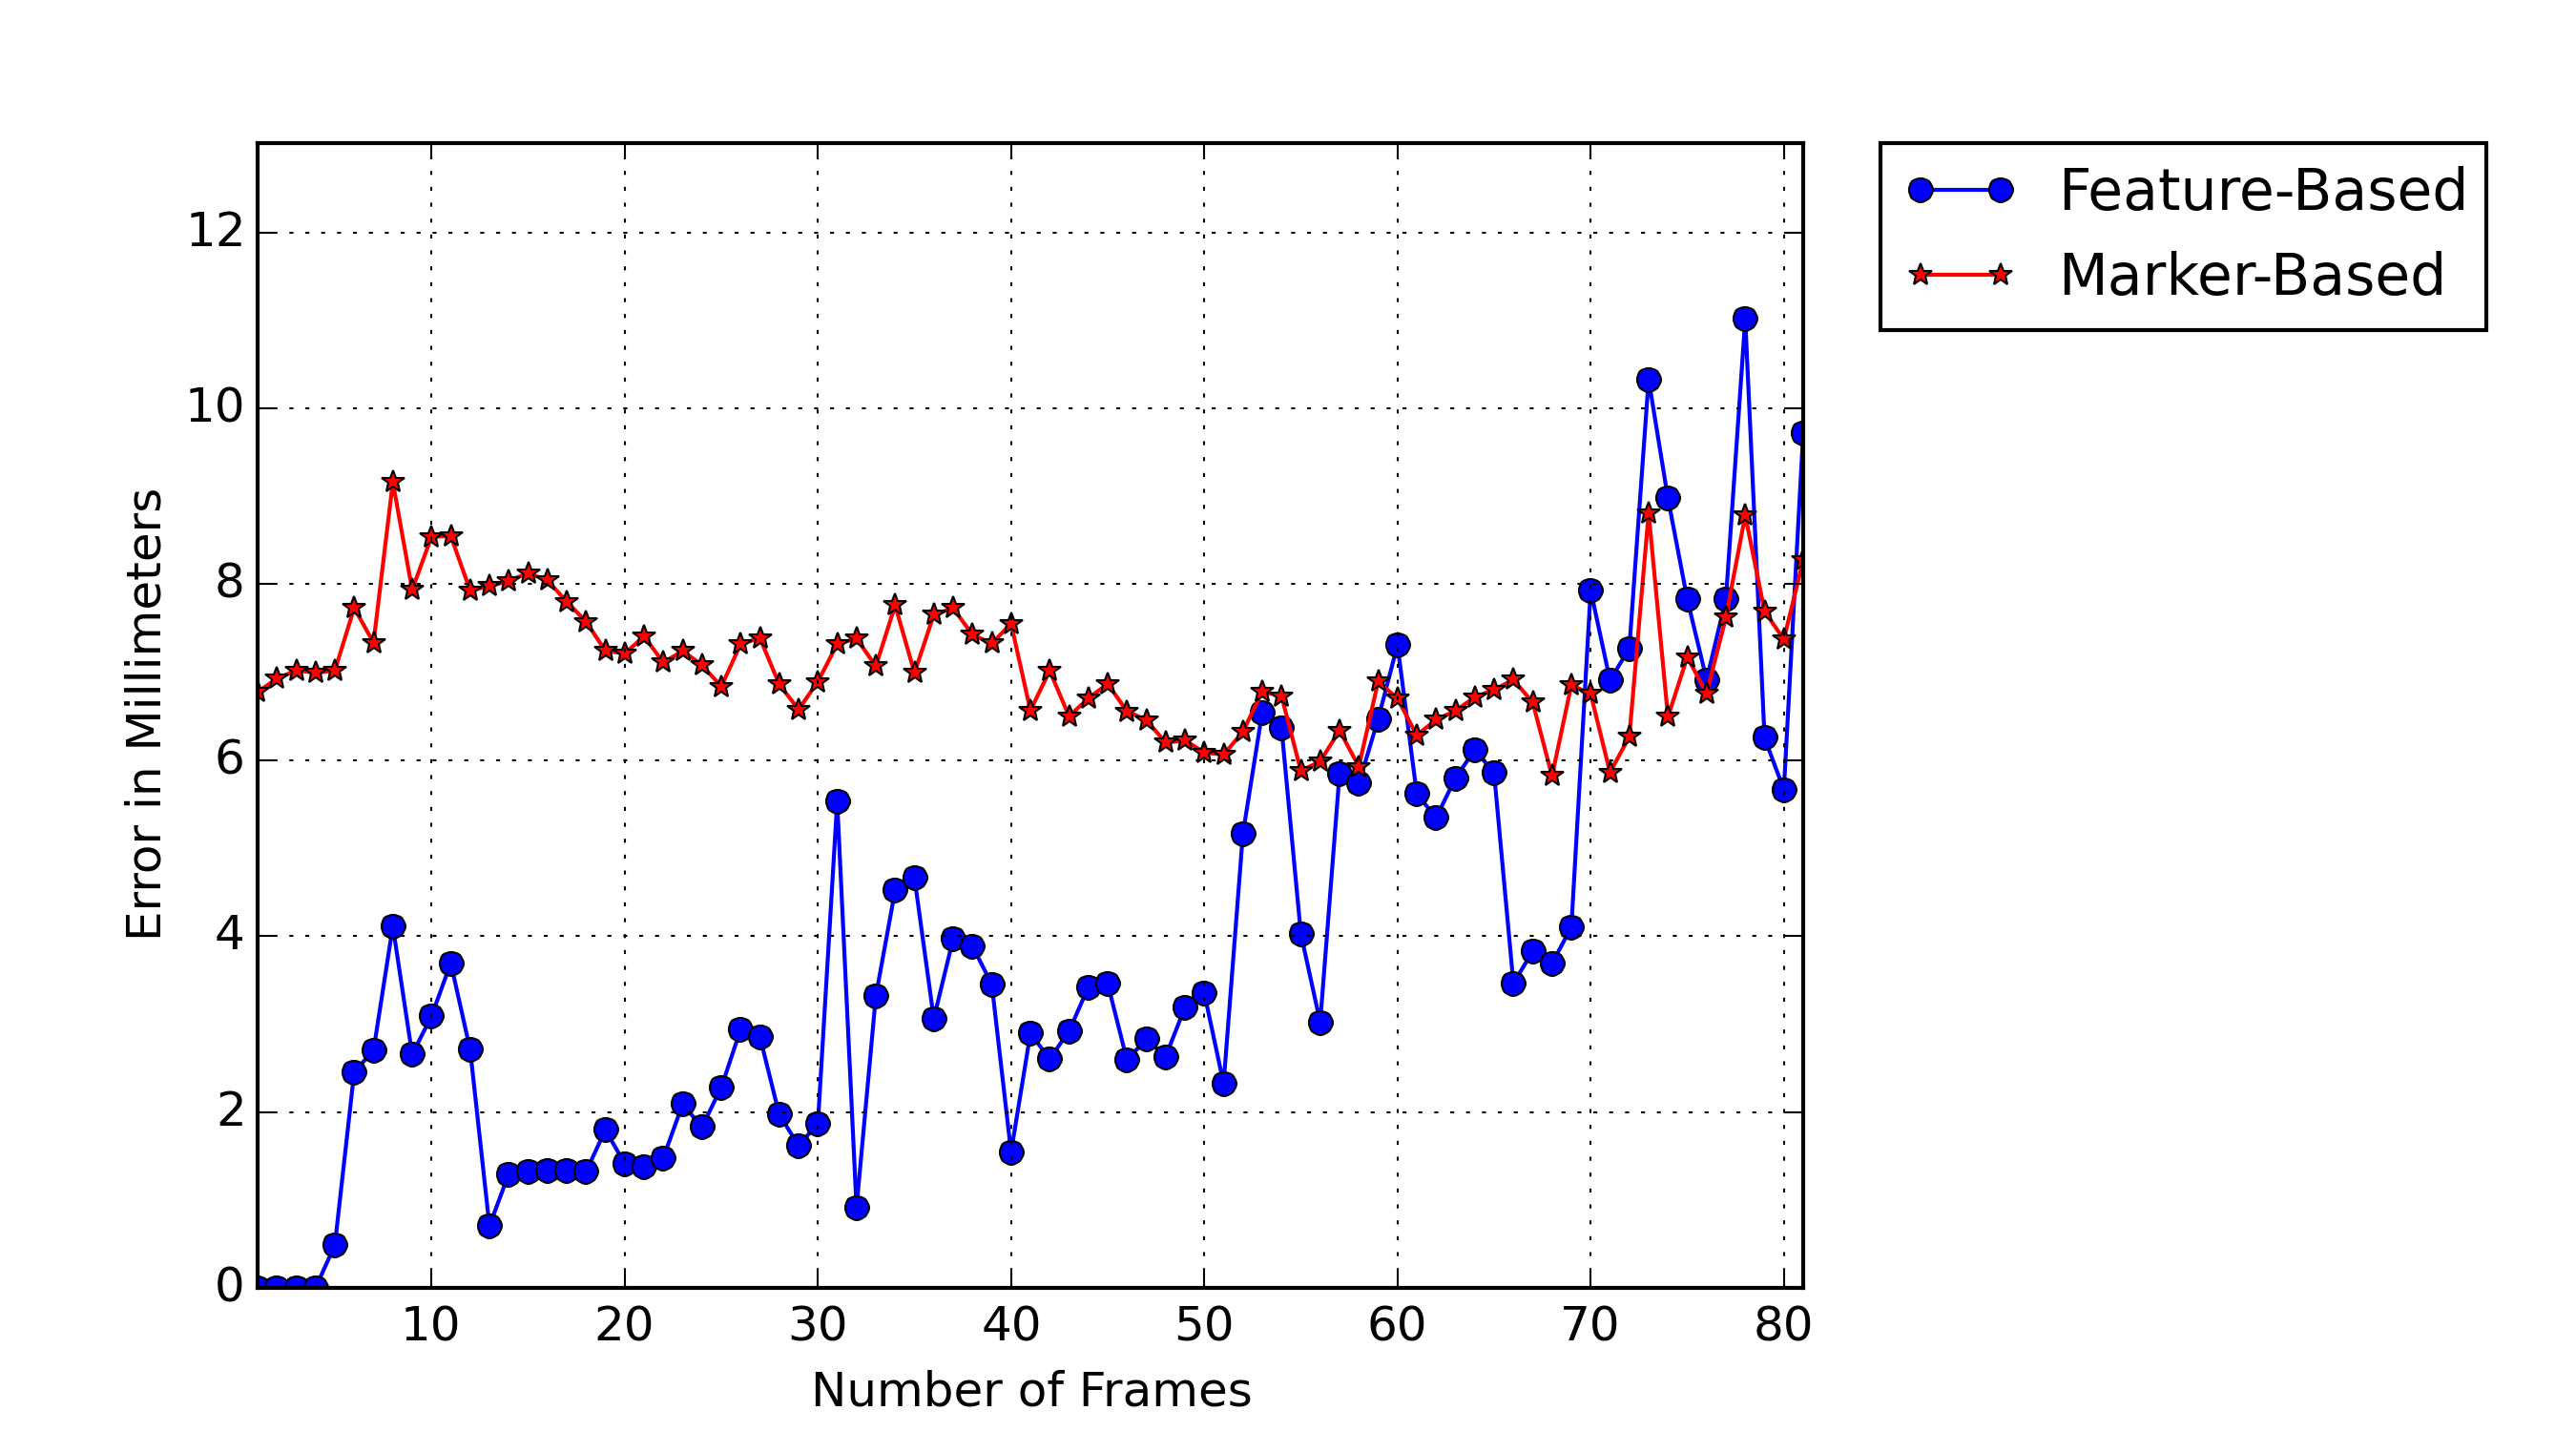
\includegraphics[width=80mm]{figures/frame_400/graph_translation} &  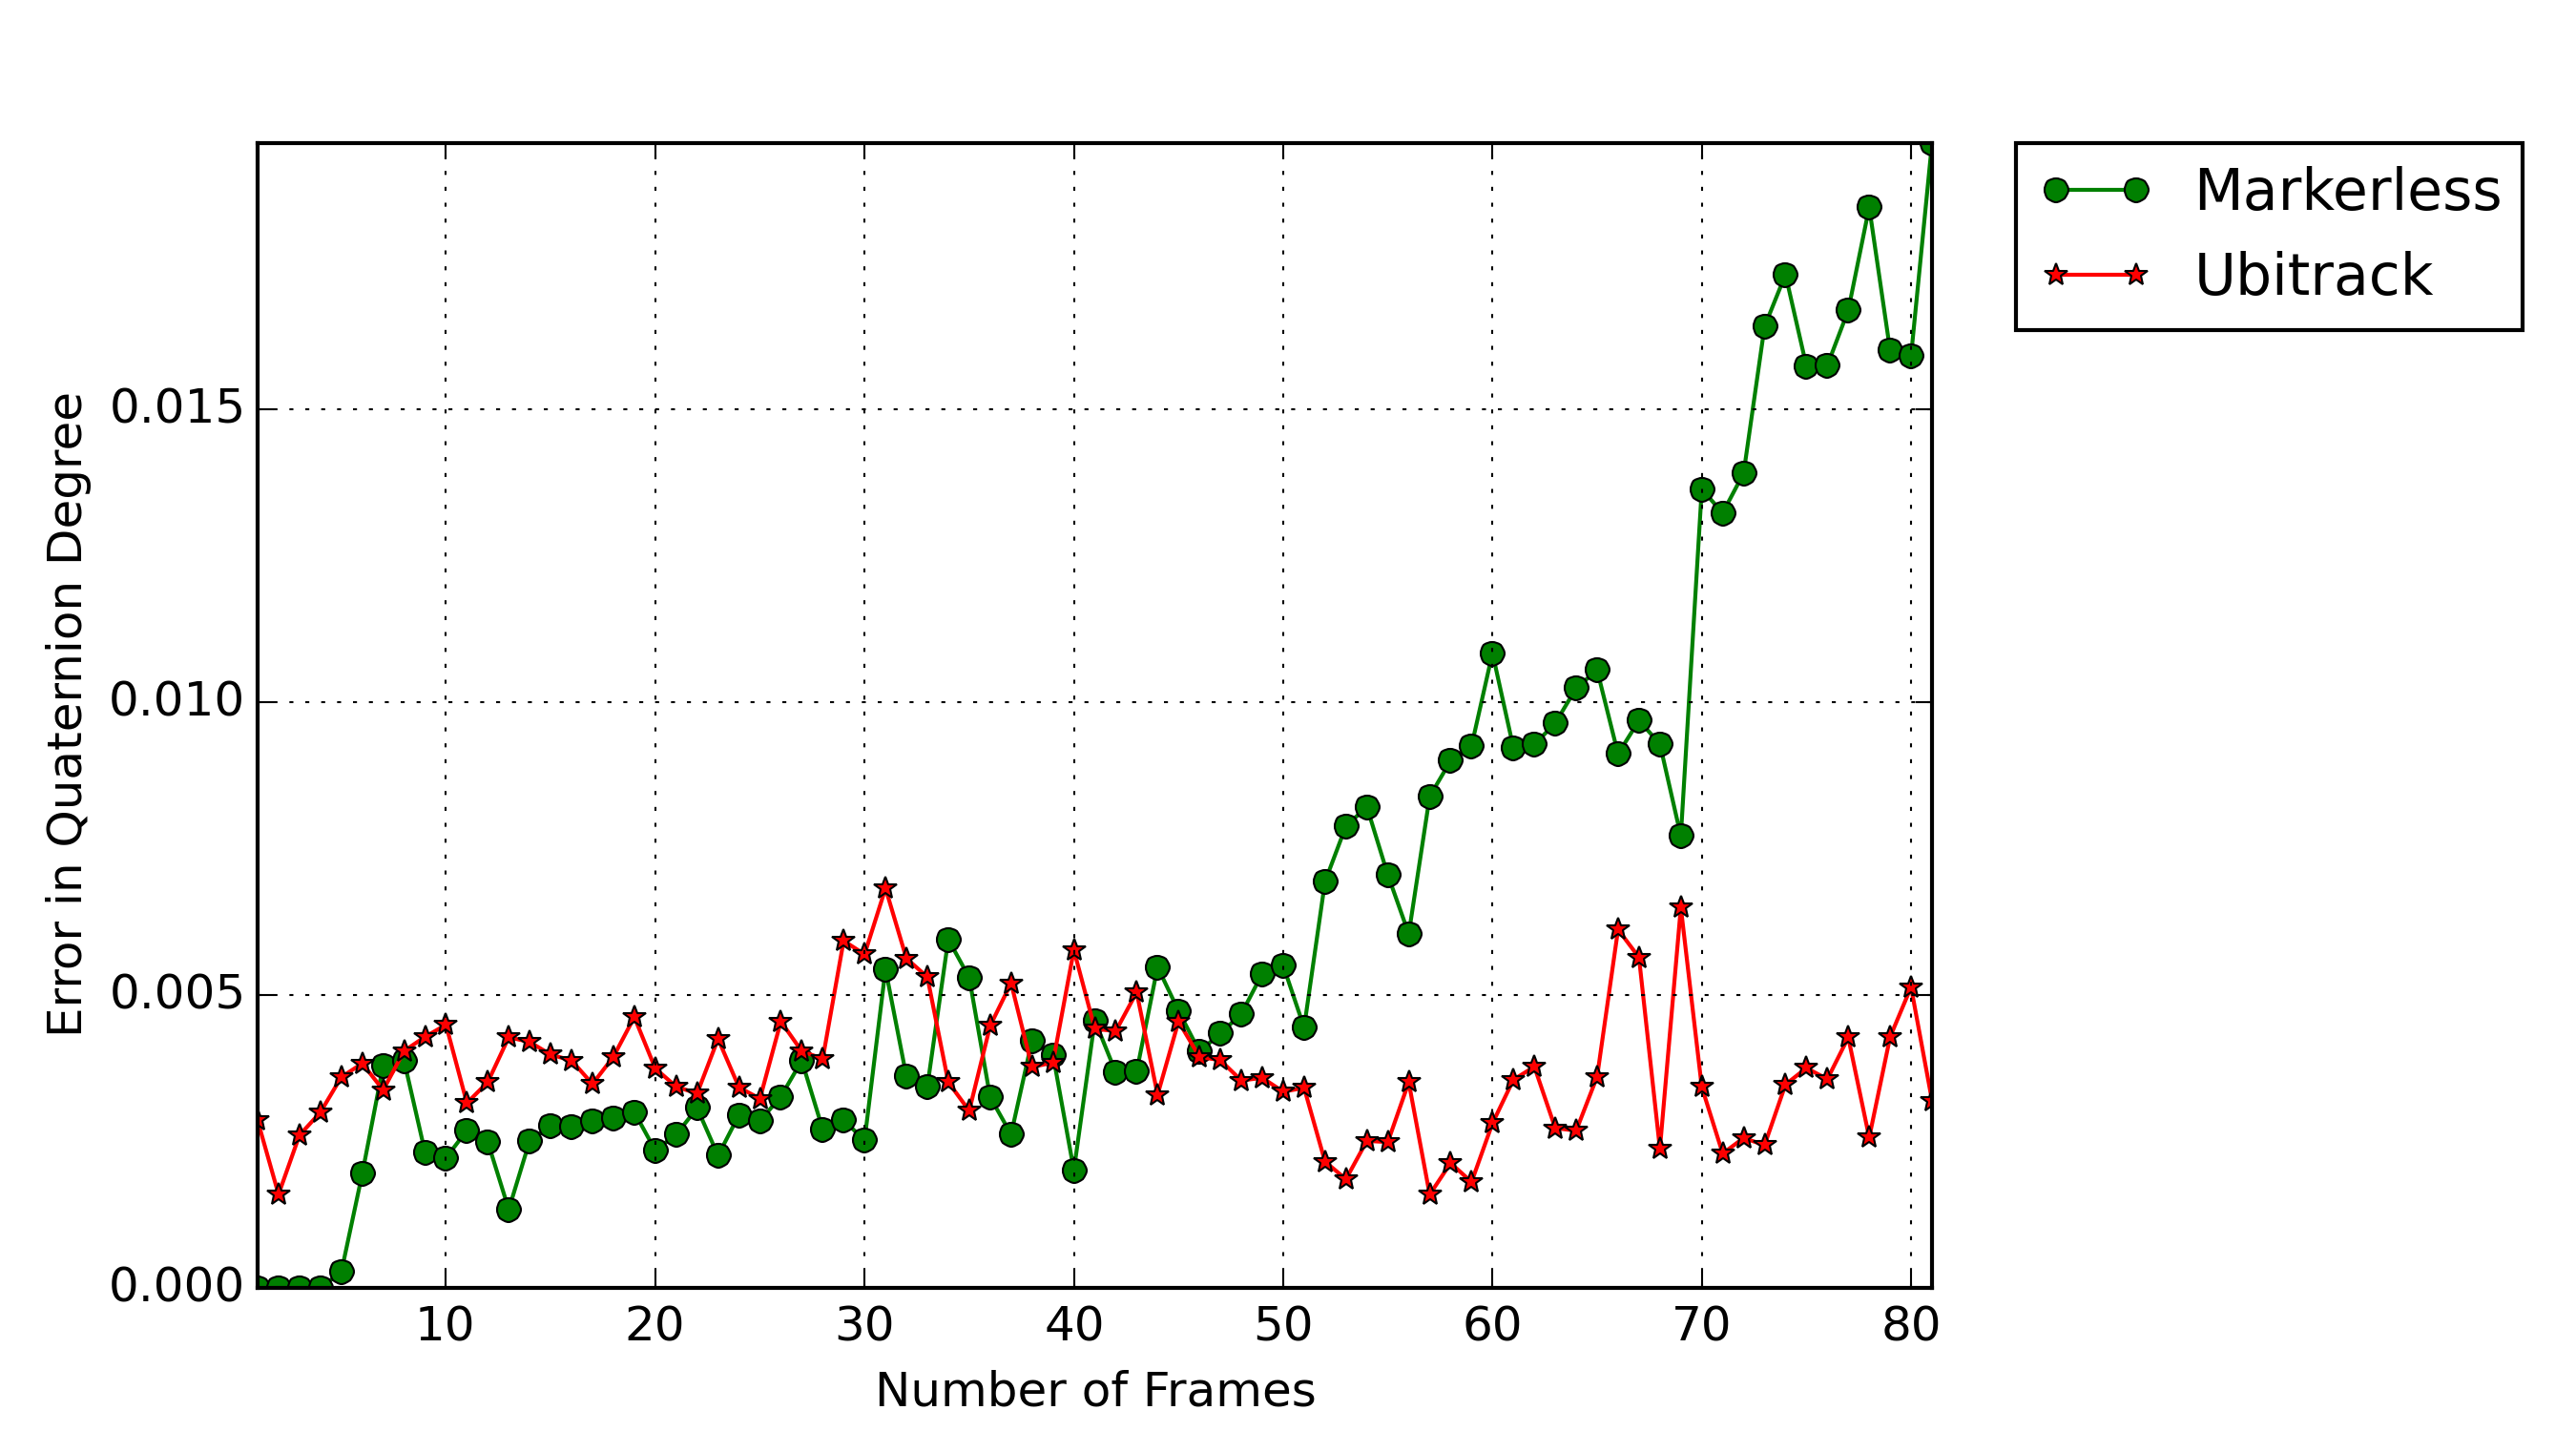
\includegraphics[width=80mm]{figures/frame_400/graph_rotation} \\
(a) the translation error in millimeters & (b) the rotation error in quaternion degree \\[6pt]
\end{tabular}
\caption{The tracking errors for both feature-based and marker-based techniques based on the second ground truth data set}\label{fig:sample_02}
\end{figure}

\begin{table}[H]
\centering
  \begin{tabular}{| c || c | c | c | c |}
      \hline
      & \multicolumn{2}{c|}{Translation} & \multicolumn{2}{c|}{Rotation} \\ \hline
       & Mean & Standard Deviation & Mean & Standard Deviation \\ \hline
      Feature-Based Approach & 3.8357 & 2.4783 & 0.0063 & 0.0049 \\ \hline
      Marker-Base Approach & 7.0932 & 0.7227 & 0.0037 & 0.0011 \\ \hline
  \end{tabular}
  \caption{the statistical analysis of tracking error for both feature-based and marker-based techniques based on the second ground truth data set} \label{tab:sample_02}
\end{table}

\autoref{tab:sample_02} and \autoref{fig:sample_02} show the result of comparison of translation and rotation errors with the ground truth for the second sample data set. The result of rotation column of \autoref{tab:sample_02} and \autoref{fig:sample_02}(b) represent a very important event in this master thesis. They show that for some data sets, the rotation estimation and optimization does not work as well as the translation estimation. 
It might be the result of two things: observing a huge rotation that our pose estimation and our PnP solver can not handle it or bad estimation for the rotation of one frame that has a cumulative error on our estimated rotation and has a bad effect on our both local and global bundle adjustment.\autoref{fig:sample_02} also shows that translation and rotation have a reflective effect on each other. It means when we have a fast increase in the error rate of rotation, it consequently has a negative effect on estimating the translation. In details, the mean of translation estimations error before the 50th frames is around 1.8 millimeters, but as the rotation estimation gets worse, the translation error increases from four millimeters to ten millimeters.

\begin{figure}[H]
\begin{tabular}{cc}
  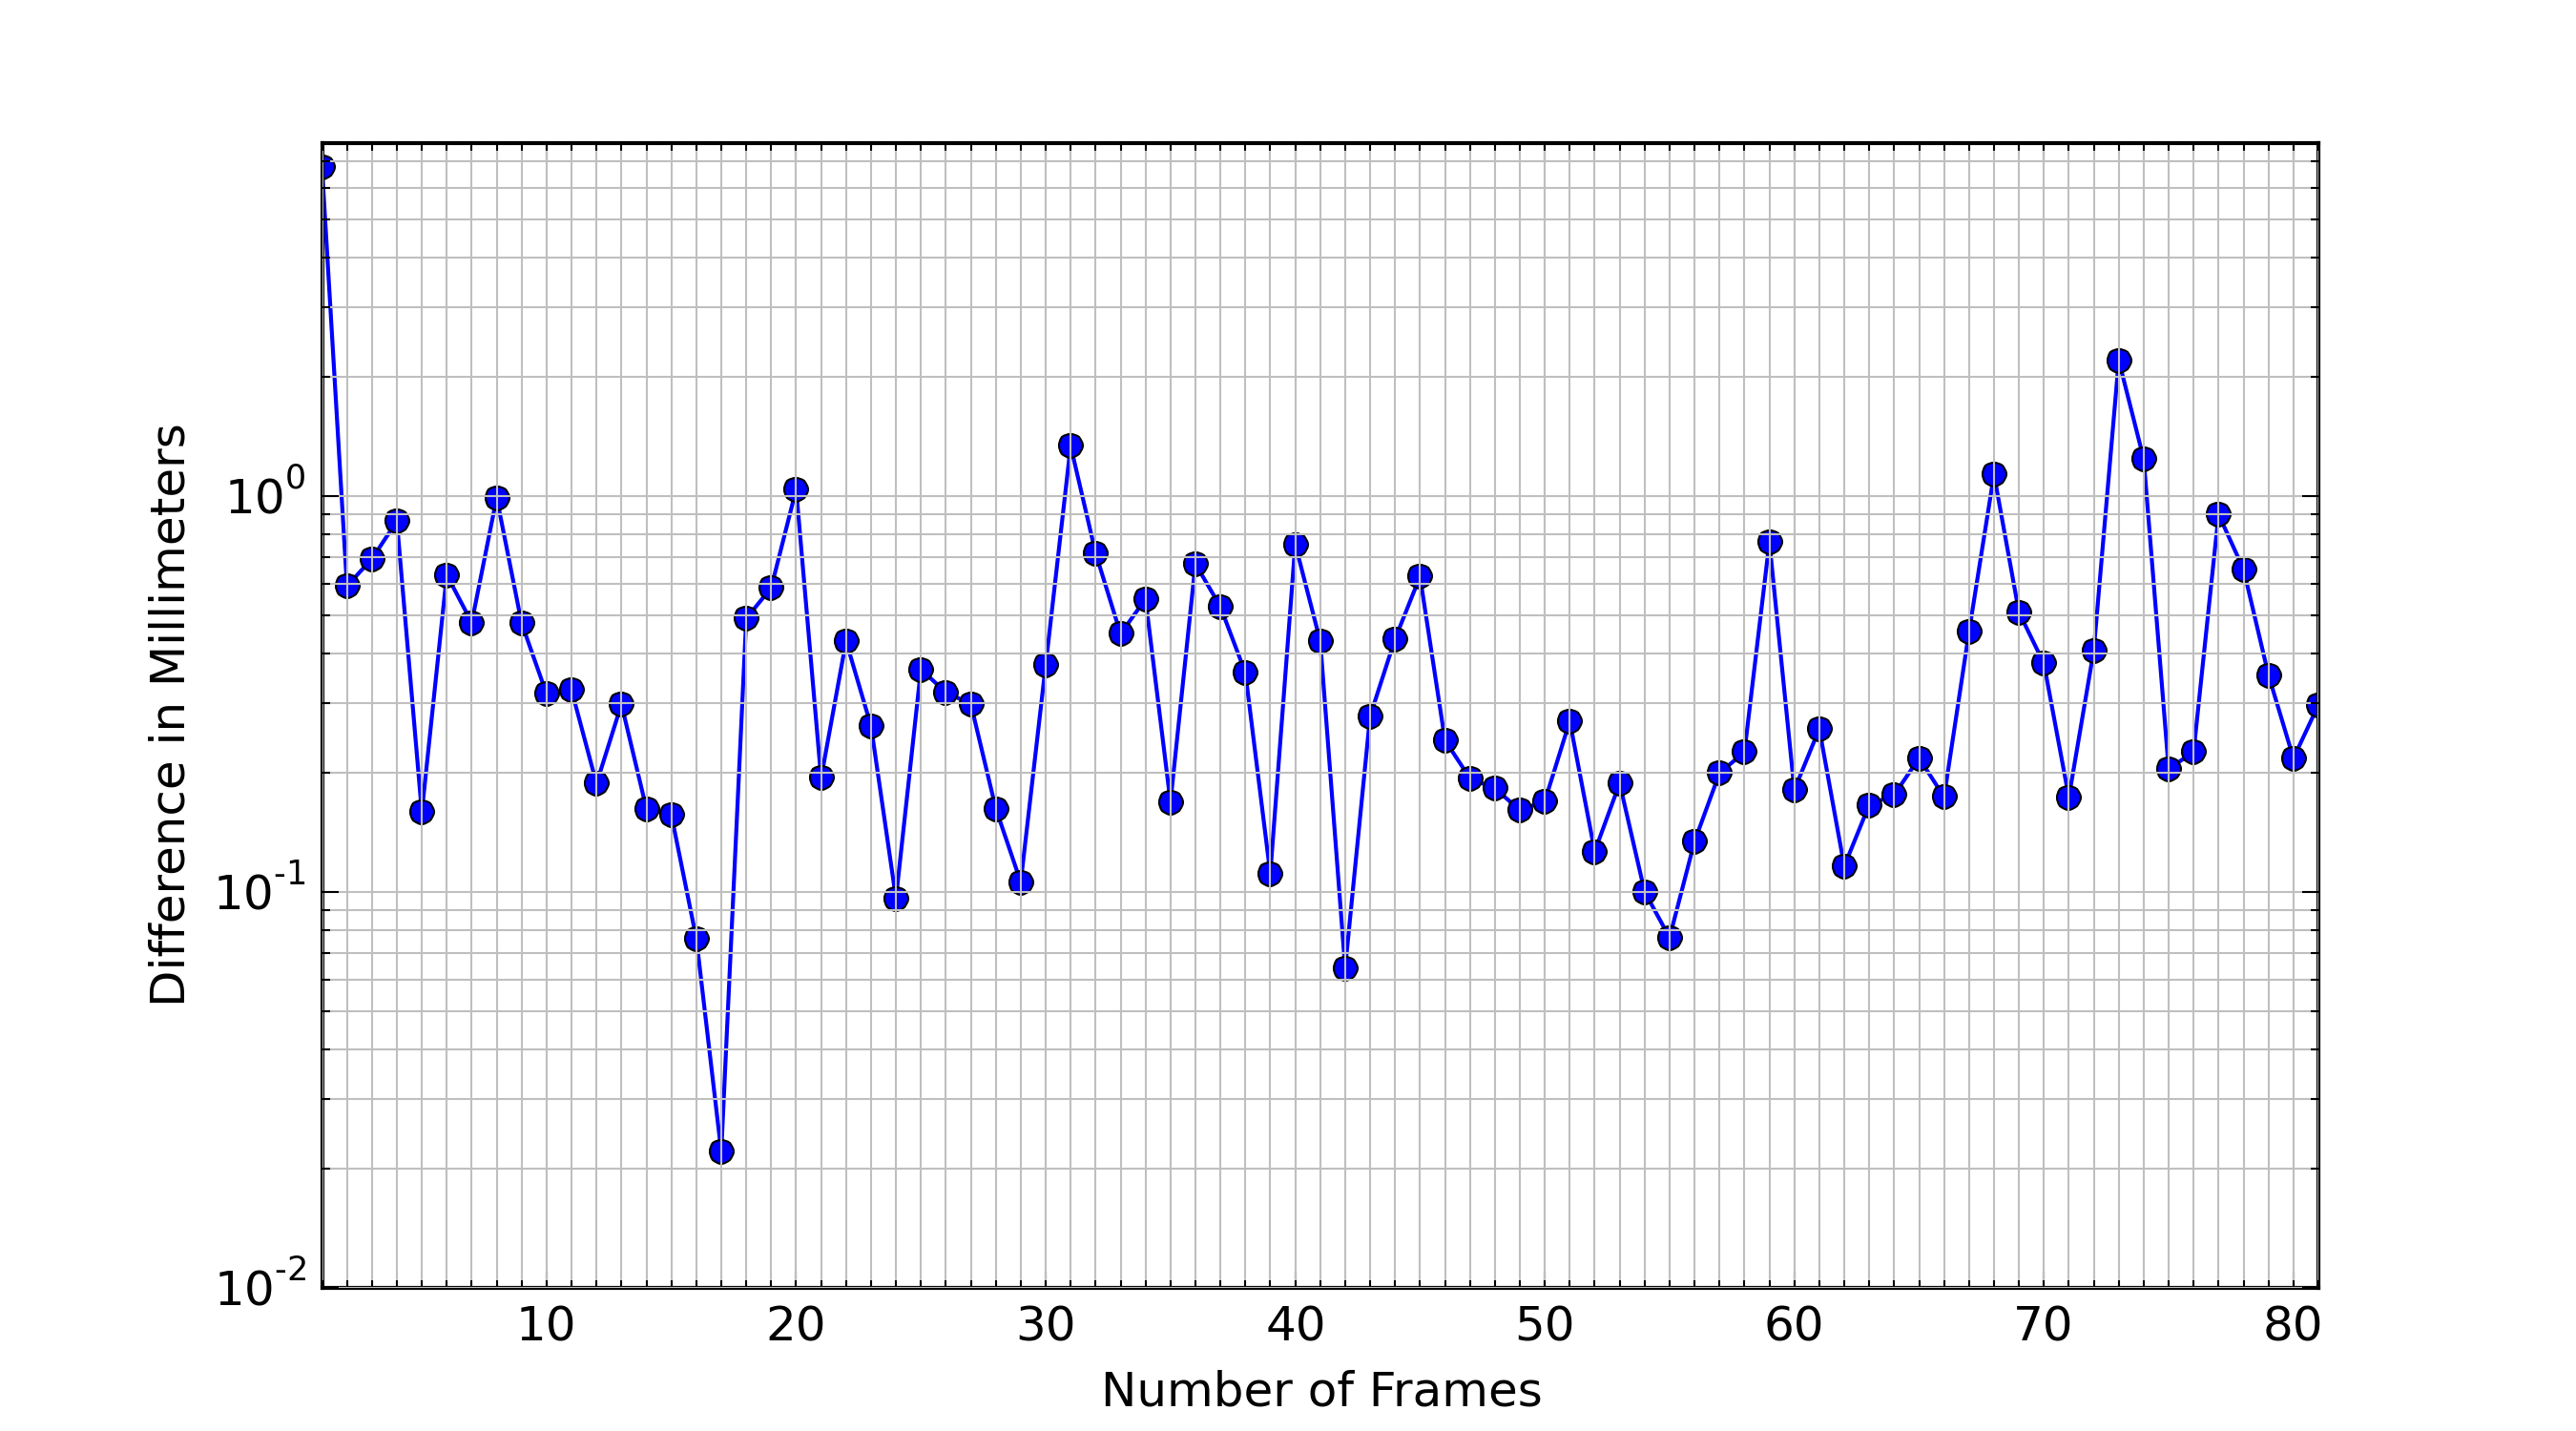
\includegraphics[width=80mm]{figures/diff_400/graph_translation} &  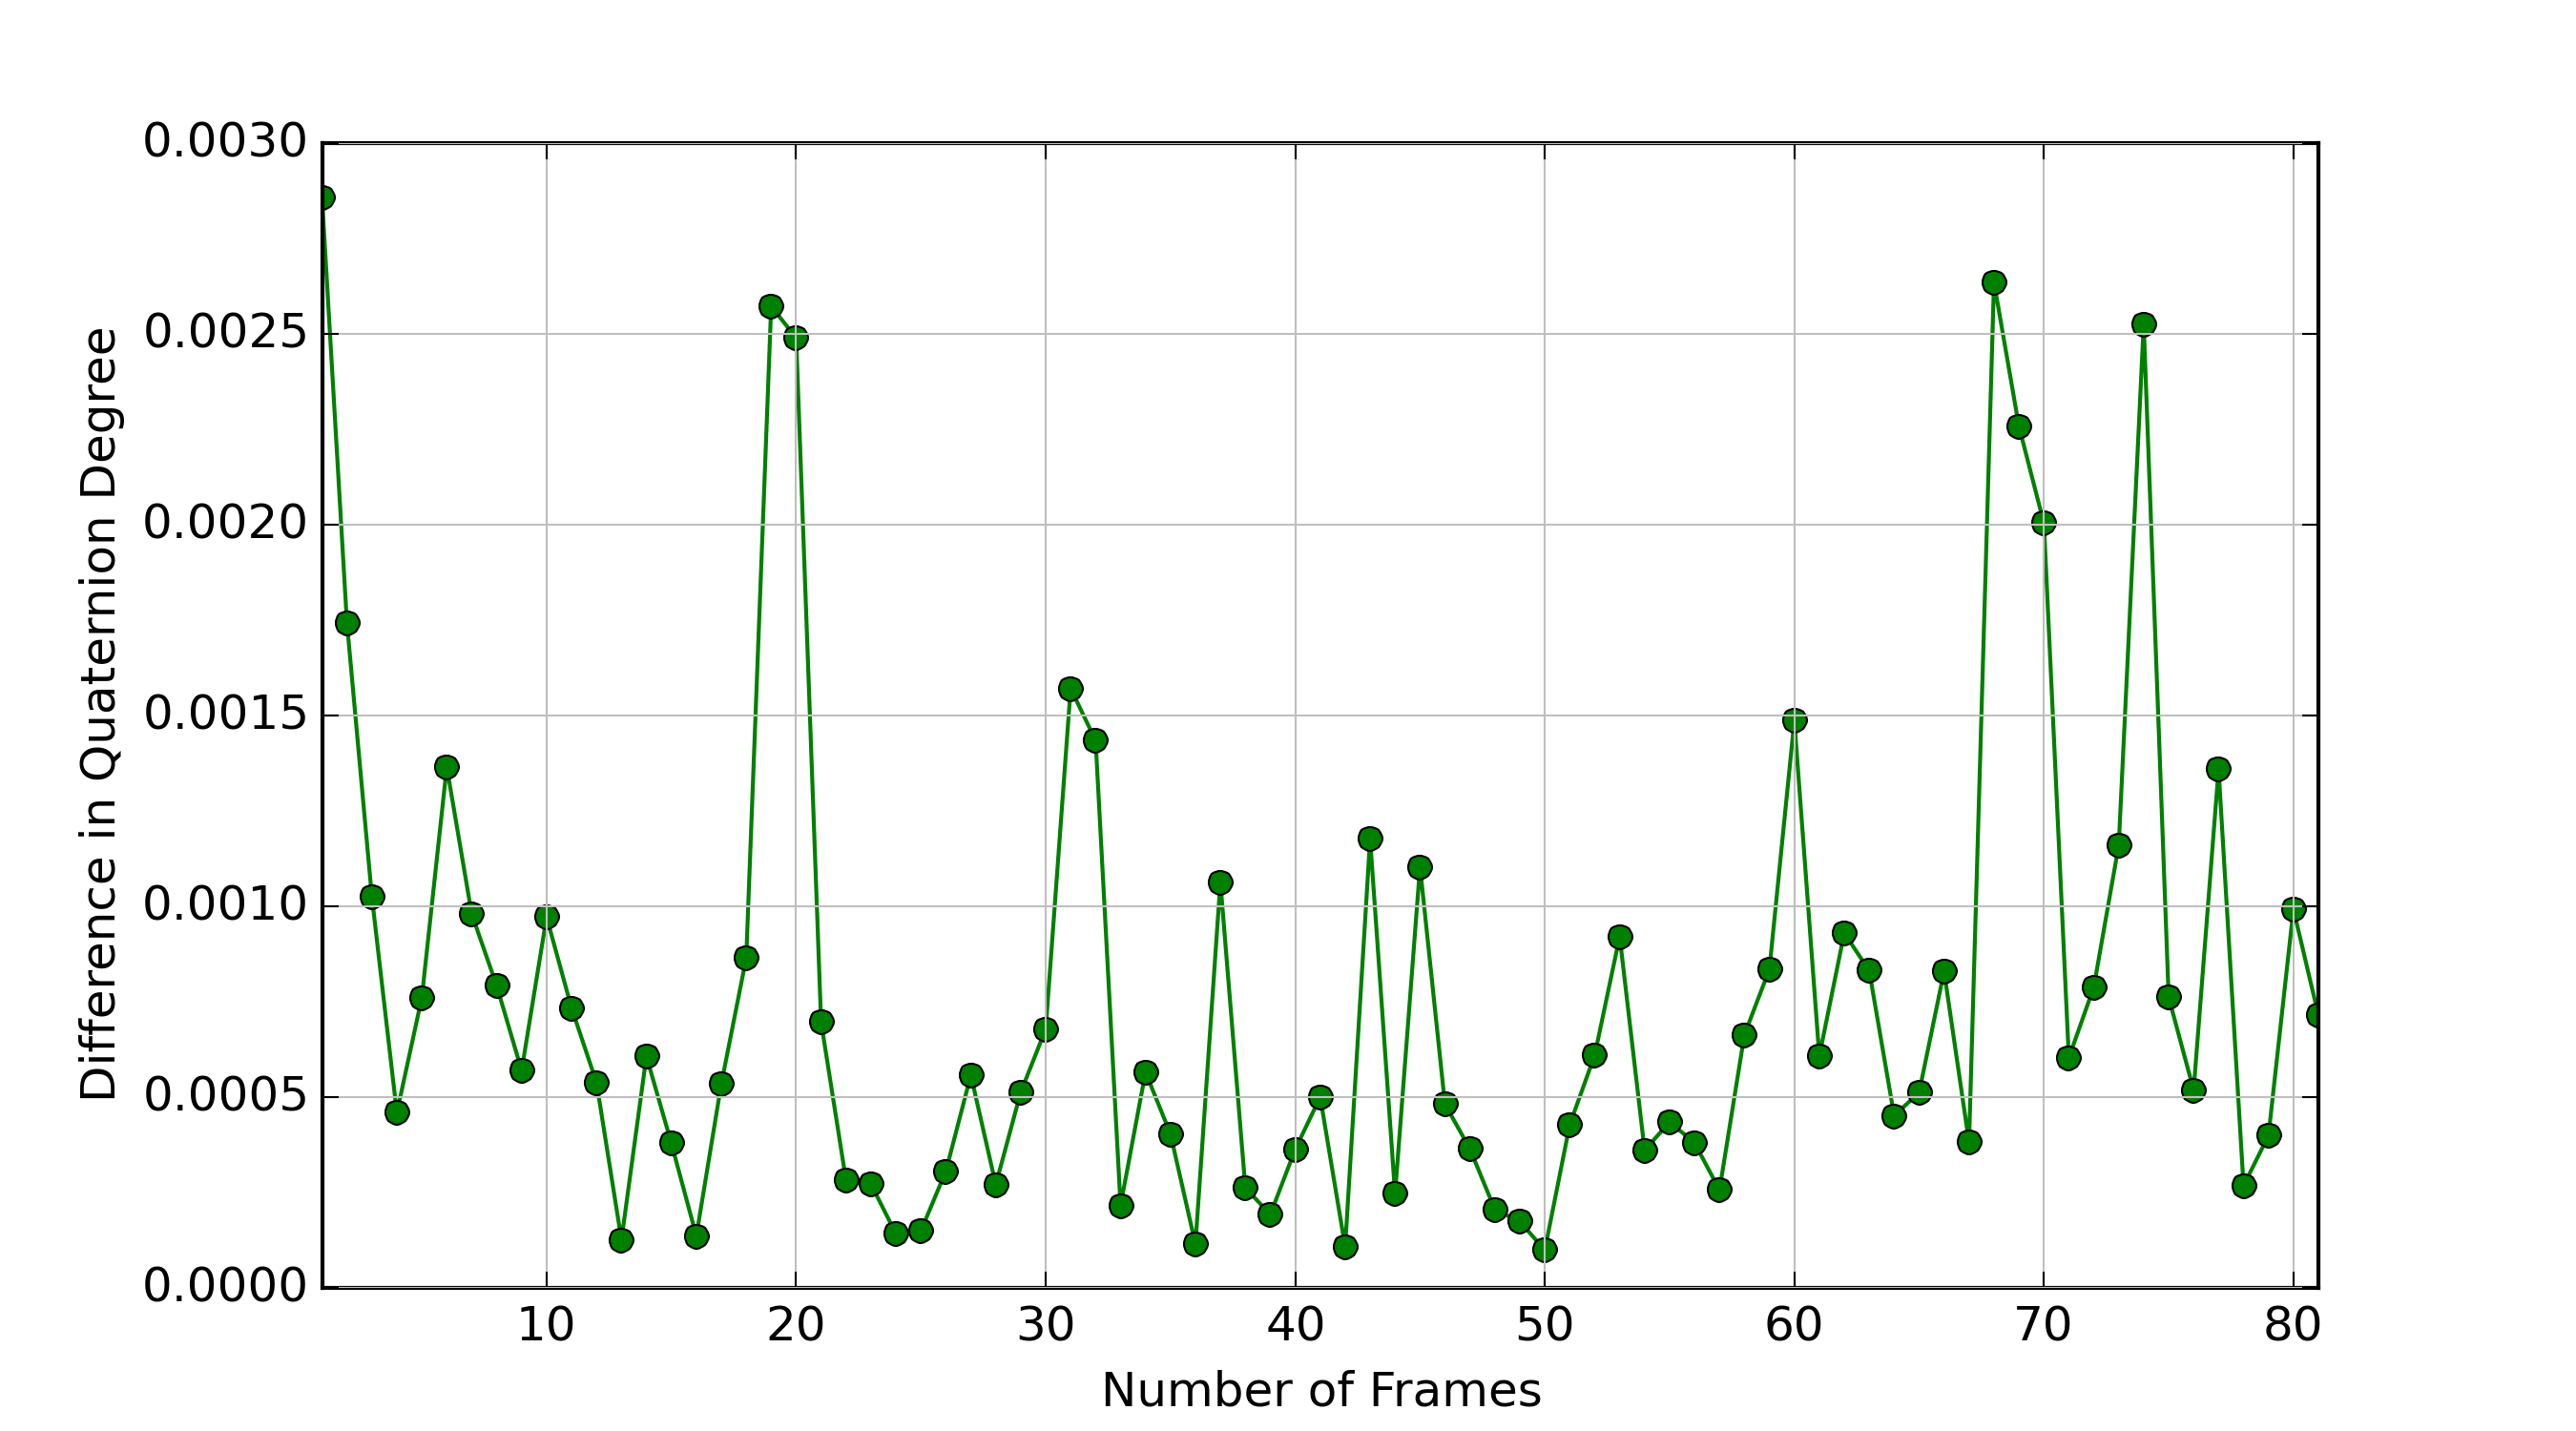
\includegraphics[width=80mm]{figures/diff_400/graph_rotation} \\
(a) difference of translation in milliliters & (b) difference of rotation in degree of quaternion \\[6pt]
\end{tabular}
\caption{The difference between the Feature-based and Marker-based for each sequence pair of second sample data set}\label{fig:sample_02_diff}
\end{figure}

\begin{table}[H]
\centering
  \begin{tabular}{| c | c | c | c |}
      \hline
      \multicolumn{2}{|c|}{Translation} & \multicolumn{2}{c}{Rotation} \\ \hline
       Mean & Standard Deviation & Mean & Standard Deviation \\ \hline
      0.4821 & 0.7839 & 0.0008 & 0.0006 \\ \hline
  \end{tabular}
  \caption{} \label{tab:sample_02_diff}
\end{table}

\section{Sample Data Set 3} \label{subsec:sample_3}
\begin{figure}[H]
\begin{tabular}{cc}
  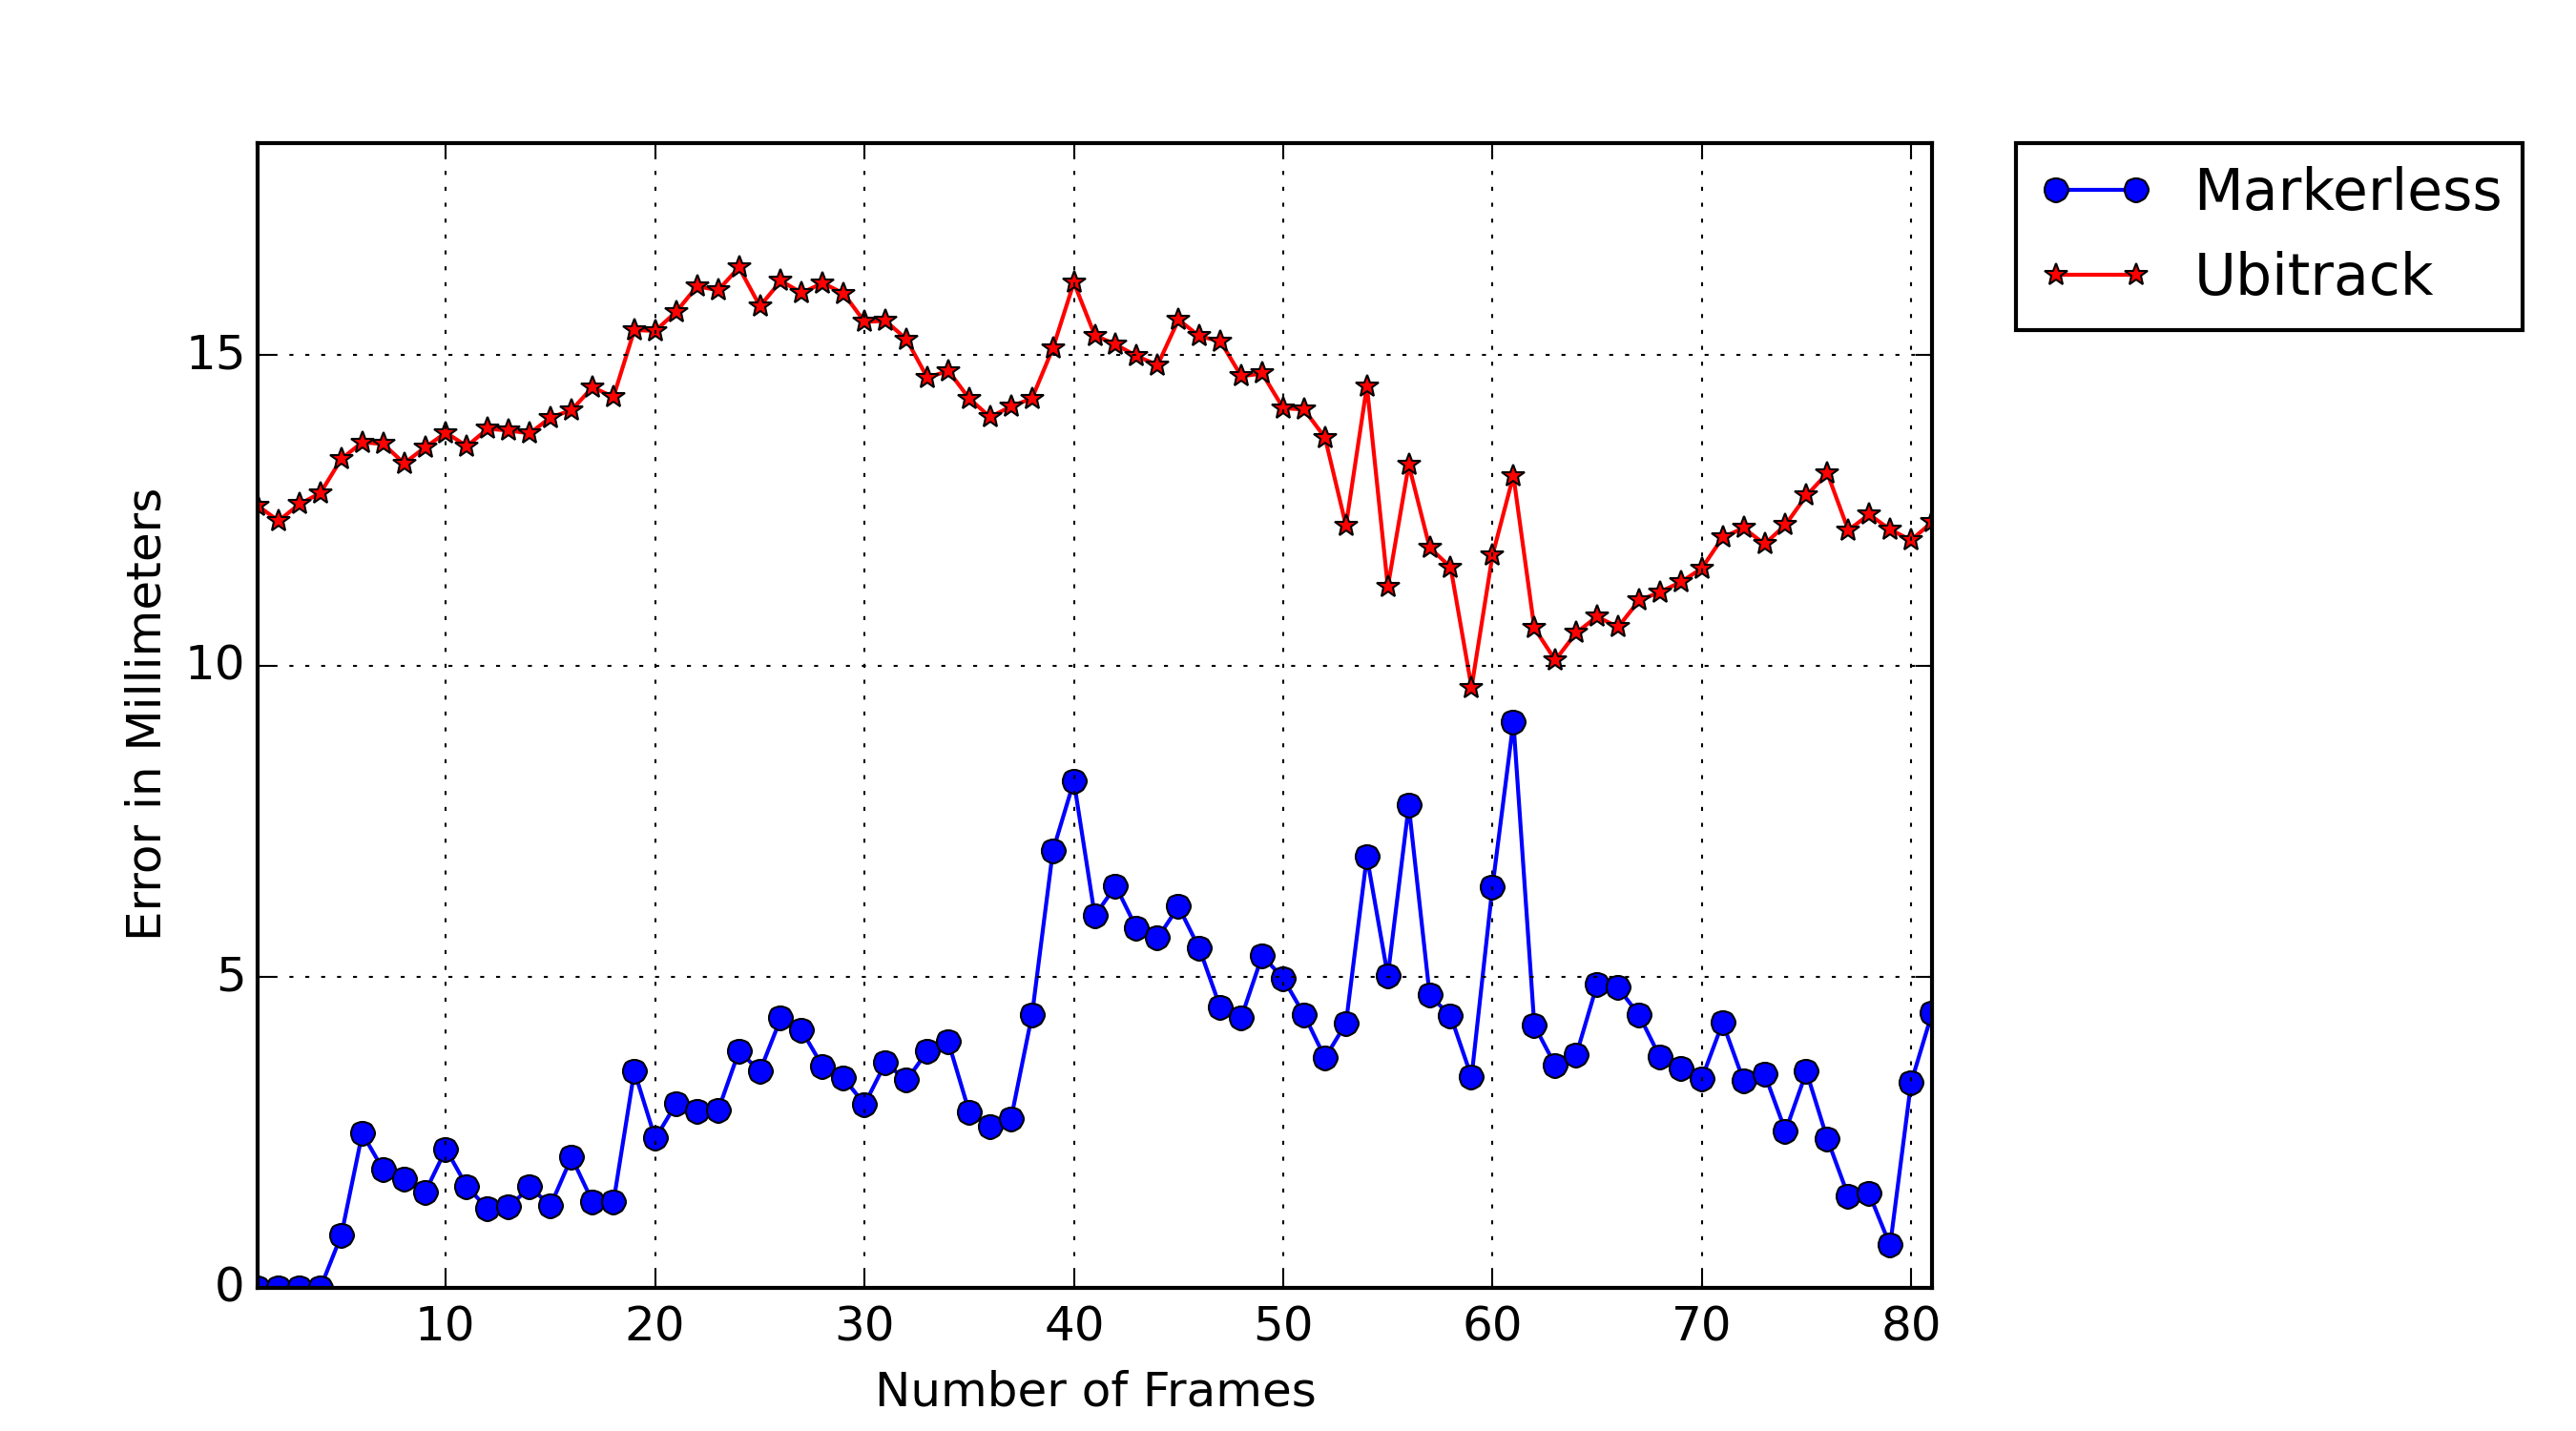
\includegraphics[width=80mm]{figures/frame_600/graph_translation} &  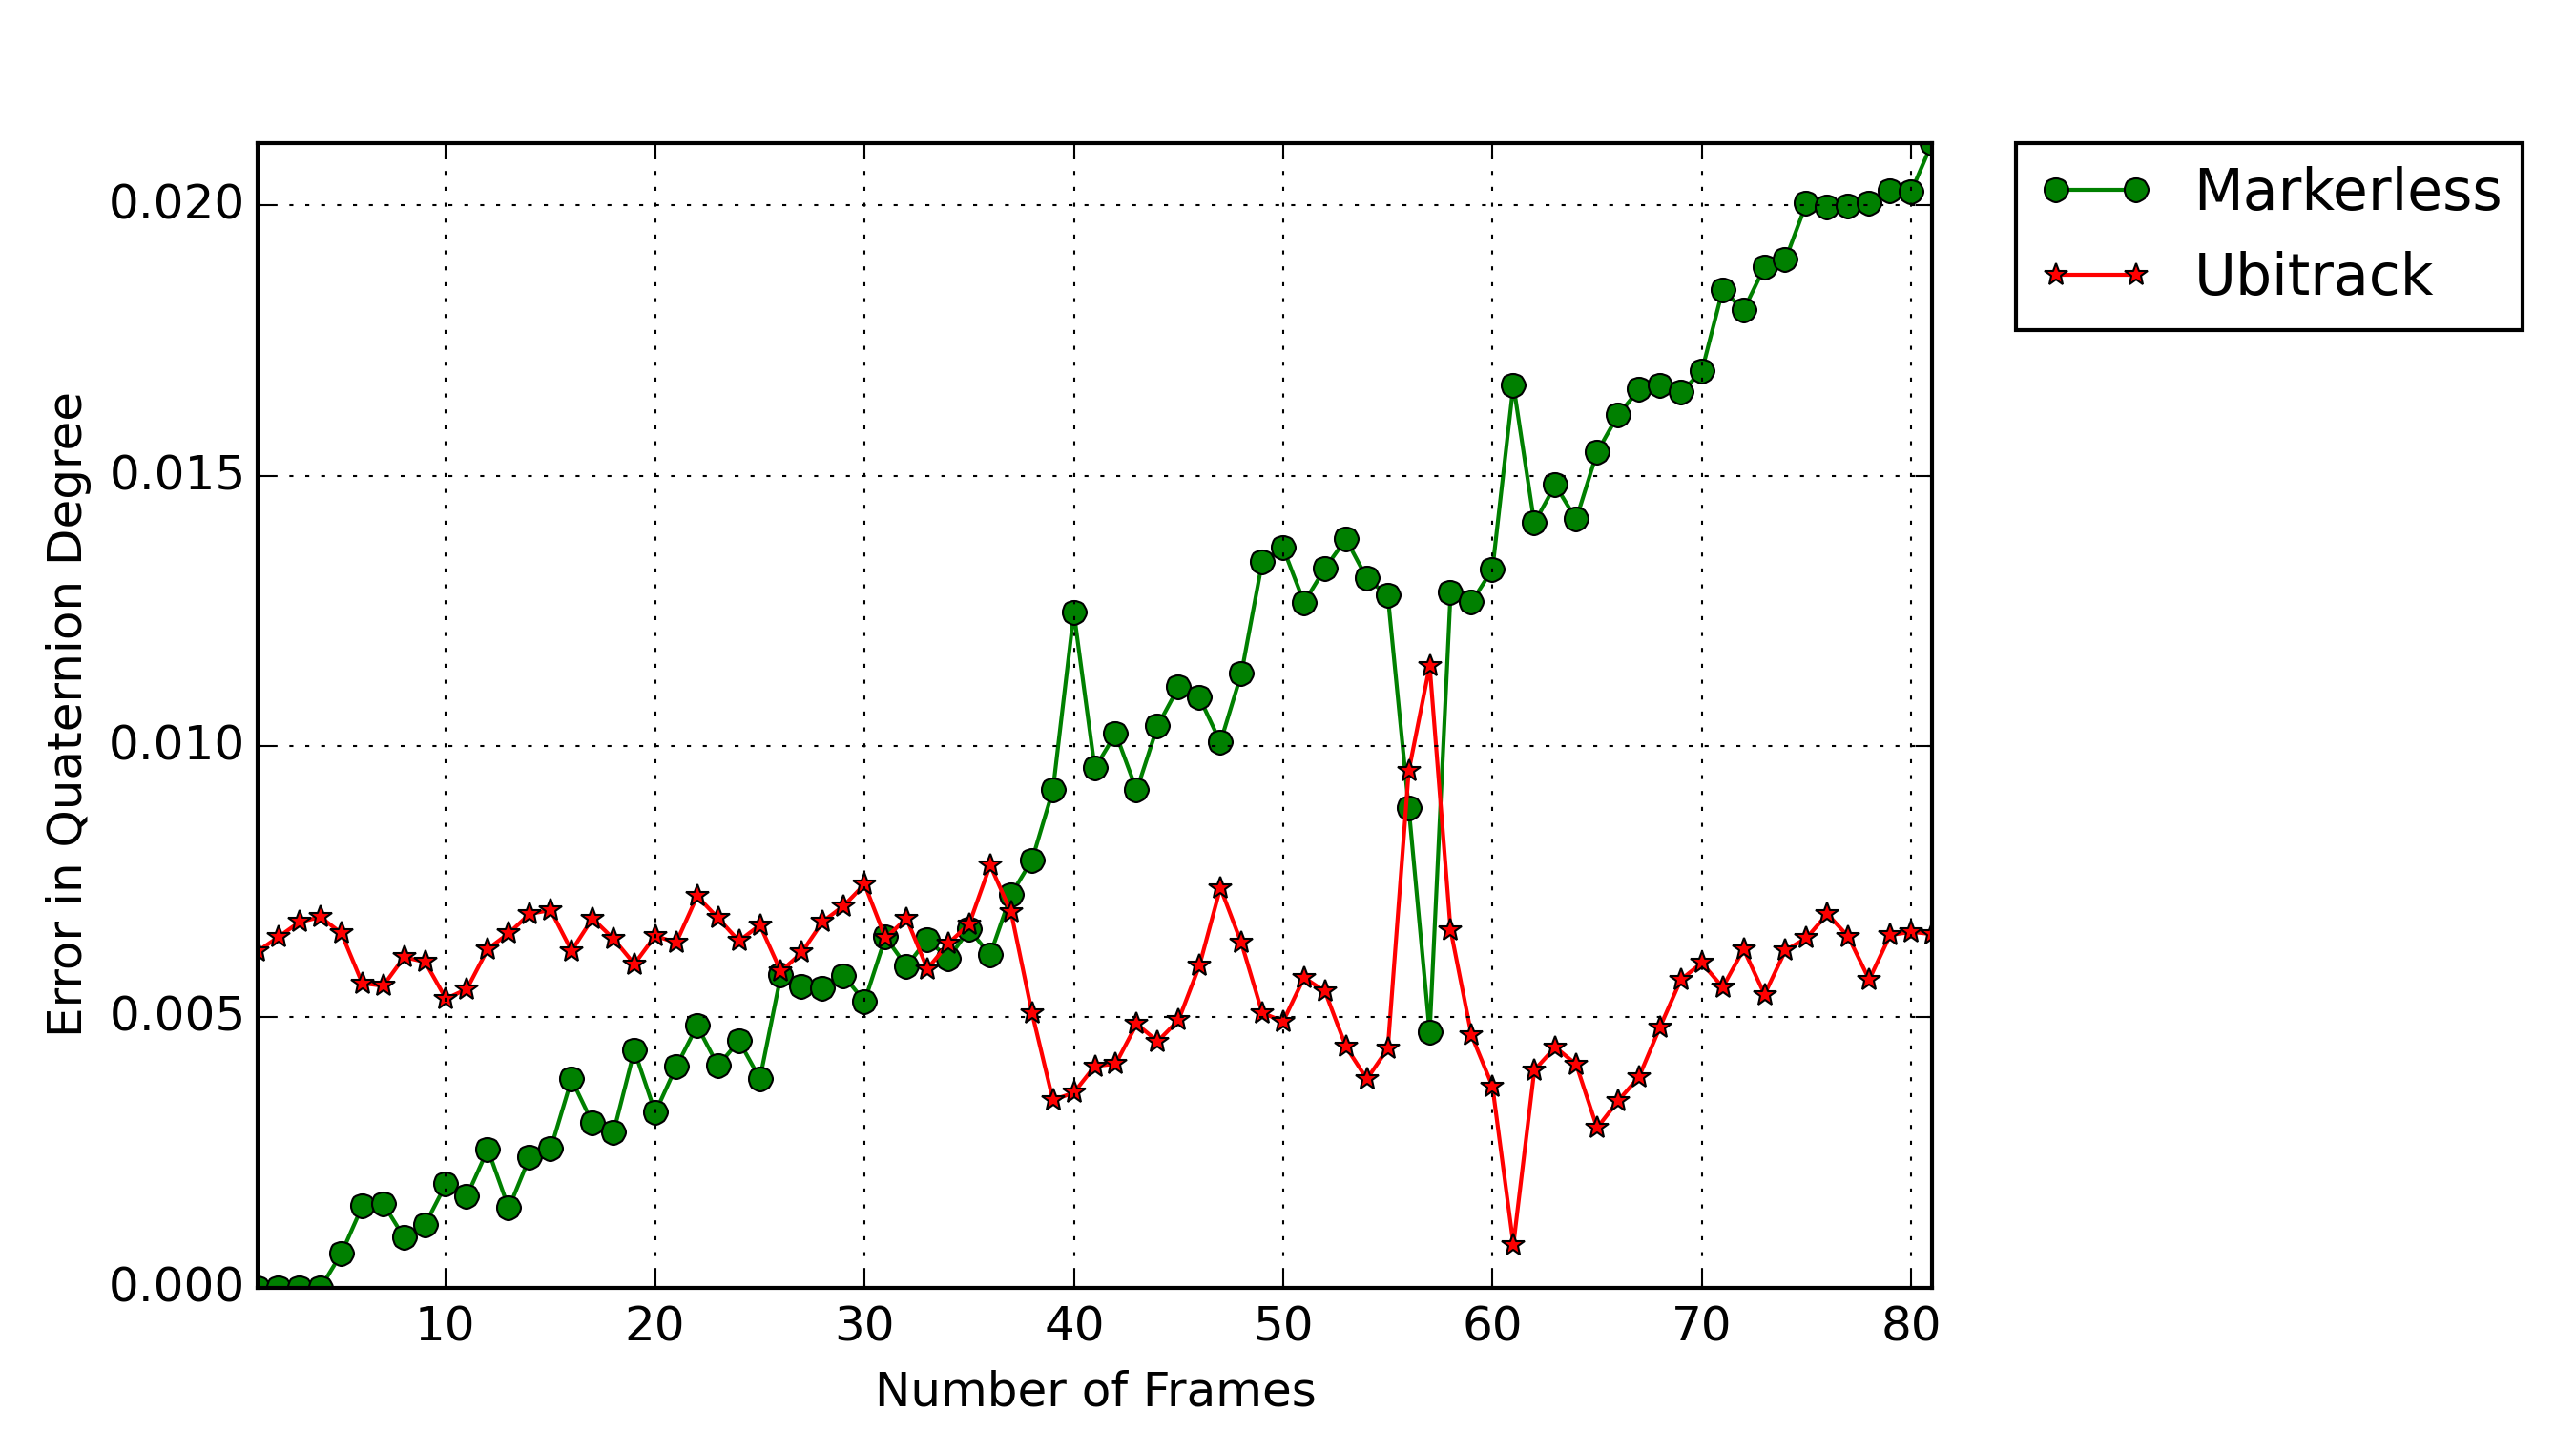
\includegraphics[width=80mm]{figures/frame_600/graph_rotation} \\
(a) translation & (b) rotation \\[6pt]
\end{tabular}
\caption{The tracking errors for both feature-based and marker-based techniques based on the third ground truth data set}\label{fig:sample_03}
\end{figure}

\begin{table}[H]
\centering
  \begin{tabular}{| c || c | c | c | c |}
      \hline
      & \multicolumn{2}{c|}{Translation} & \multicolumn{2}{c|}{Rotation} \\ \hline
       & Mean & Standard Deviation & Mean & Standard Deviation \\ \hline
      Feature-Based Approach & 3.5443 & 1.8751 & 0.0094 & 0.0063 \\ \hline
      Marker-Base Approach & 13.6084 & 1.6970 & 0.0058 & 0.0014 \\ \hline
  \end{tabular}
  \caption{the statistical analysis of tracking error for both feature-based and marker-based techniques based on the second ground truth data set} \label{tab:sample_03}
\end{table}

\autoref{tab:sample_03} and \autoref{fig:sample_03} show the result of comparison of translation and rotation errors with the ground truth for the third sample data set. These results prove that our idea about the replacing of 3D points in world map with the new one after each 35 frames was true. Let me to divide the \autoref{fig:sample_03}(a) into 3 parts. for the first seven bundles (frames 1 to 35), second seven bundles (from 36 to 70) and the rest. As you can see in \autoref{fig:sample_03}, the translation error in the first part (first seven bundles) is around the 2.5 millimeters. After that the inefficient results of the rotation that has a dramatical growth, cause the translation estimations also have a jump to the up and the mean of error is set around the 5.5 millimeters. But after the 70th frame and because the whole 3D points in world map are replaced with the new data, the local and global bundle adjustment could control the error of the translation for the next frames and bundles. In the case of rotation, once more is happened that rotation estimation and optimization are not efficient as well as the translation part.

\begin{figure}[H]
\begin{tabular}{cc}
  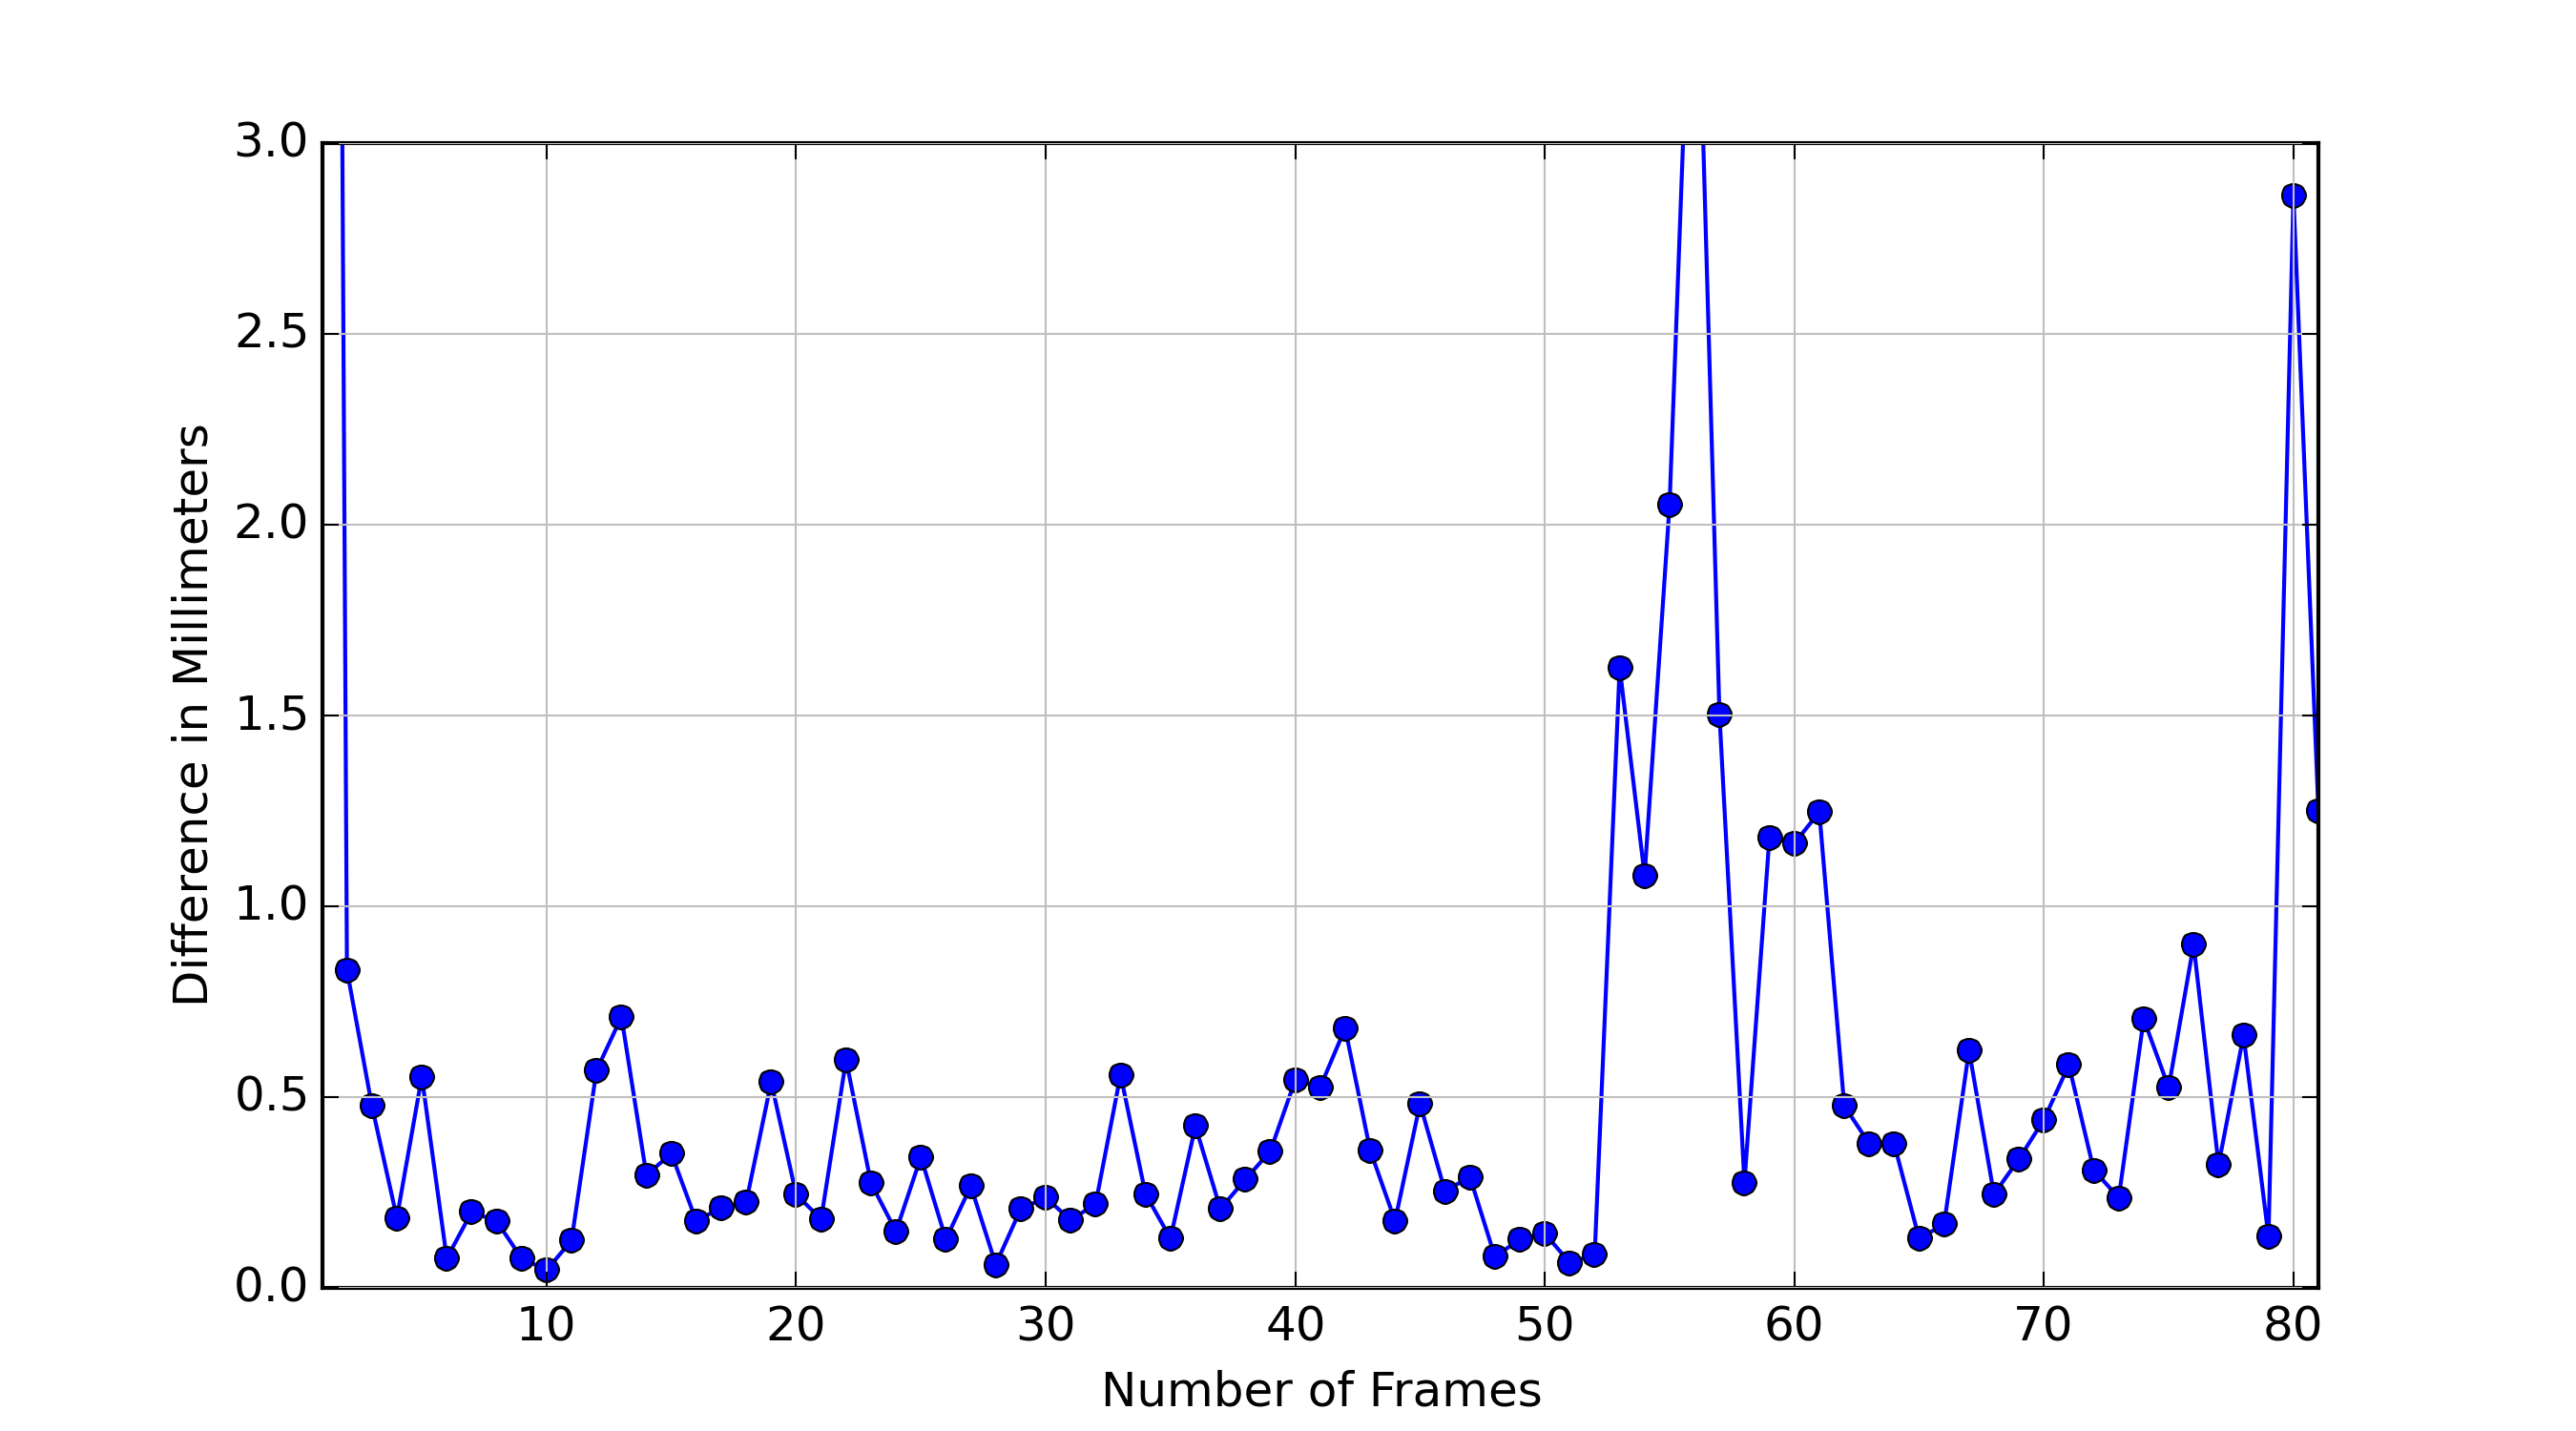
\includegraphics[width=80mm]{figures/diff_600/graph_translation} &  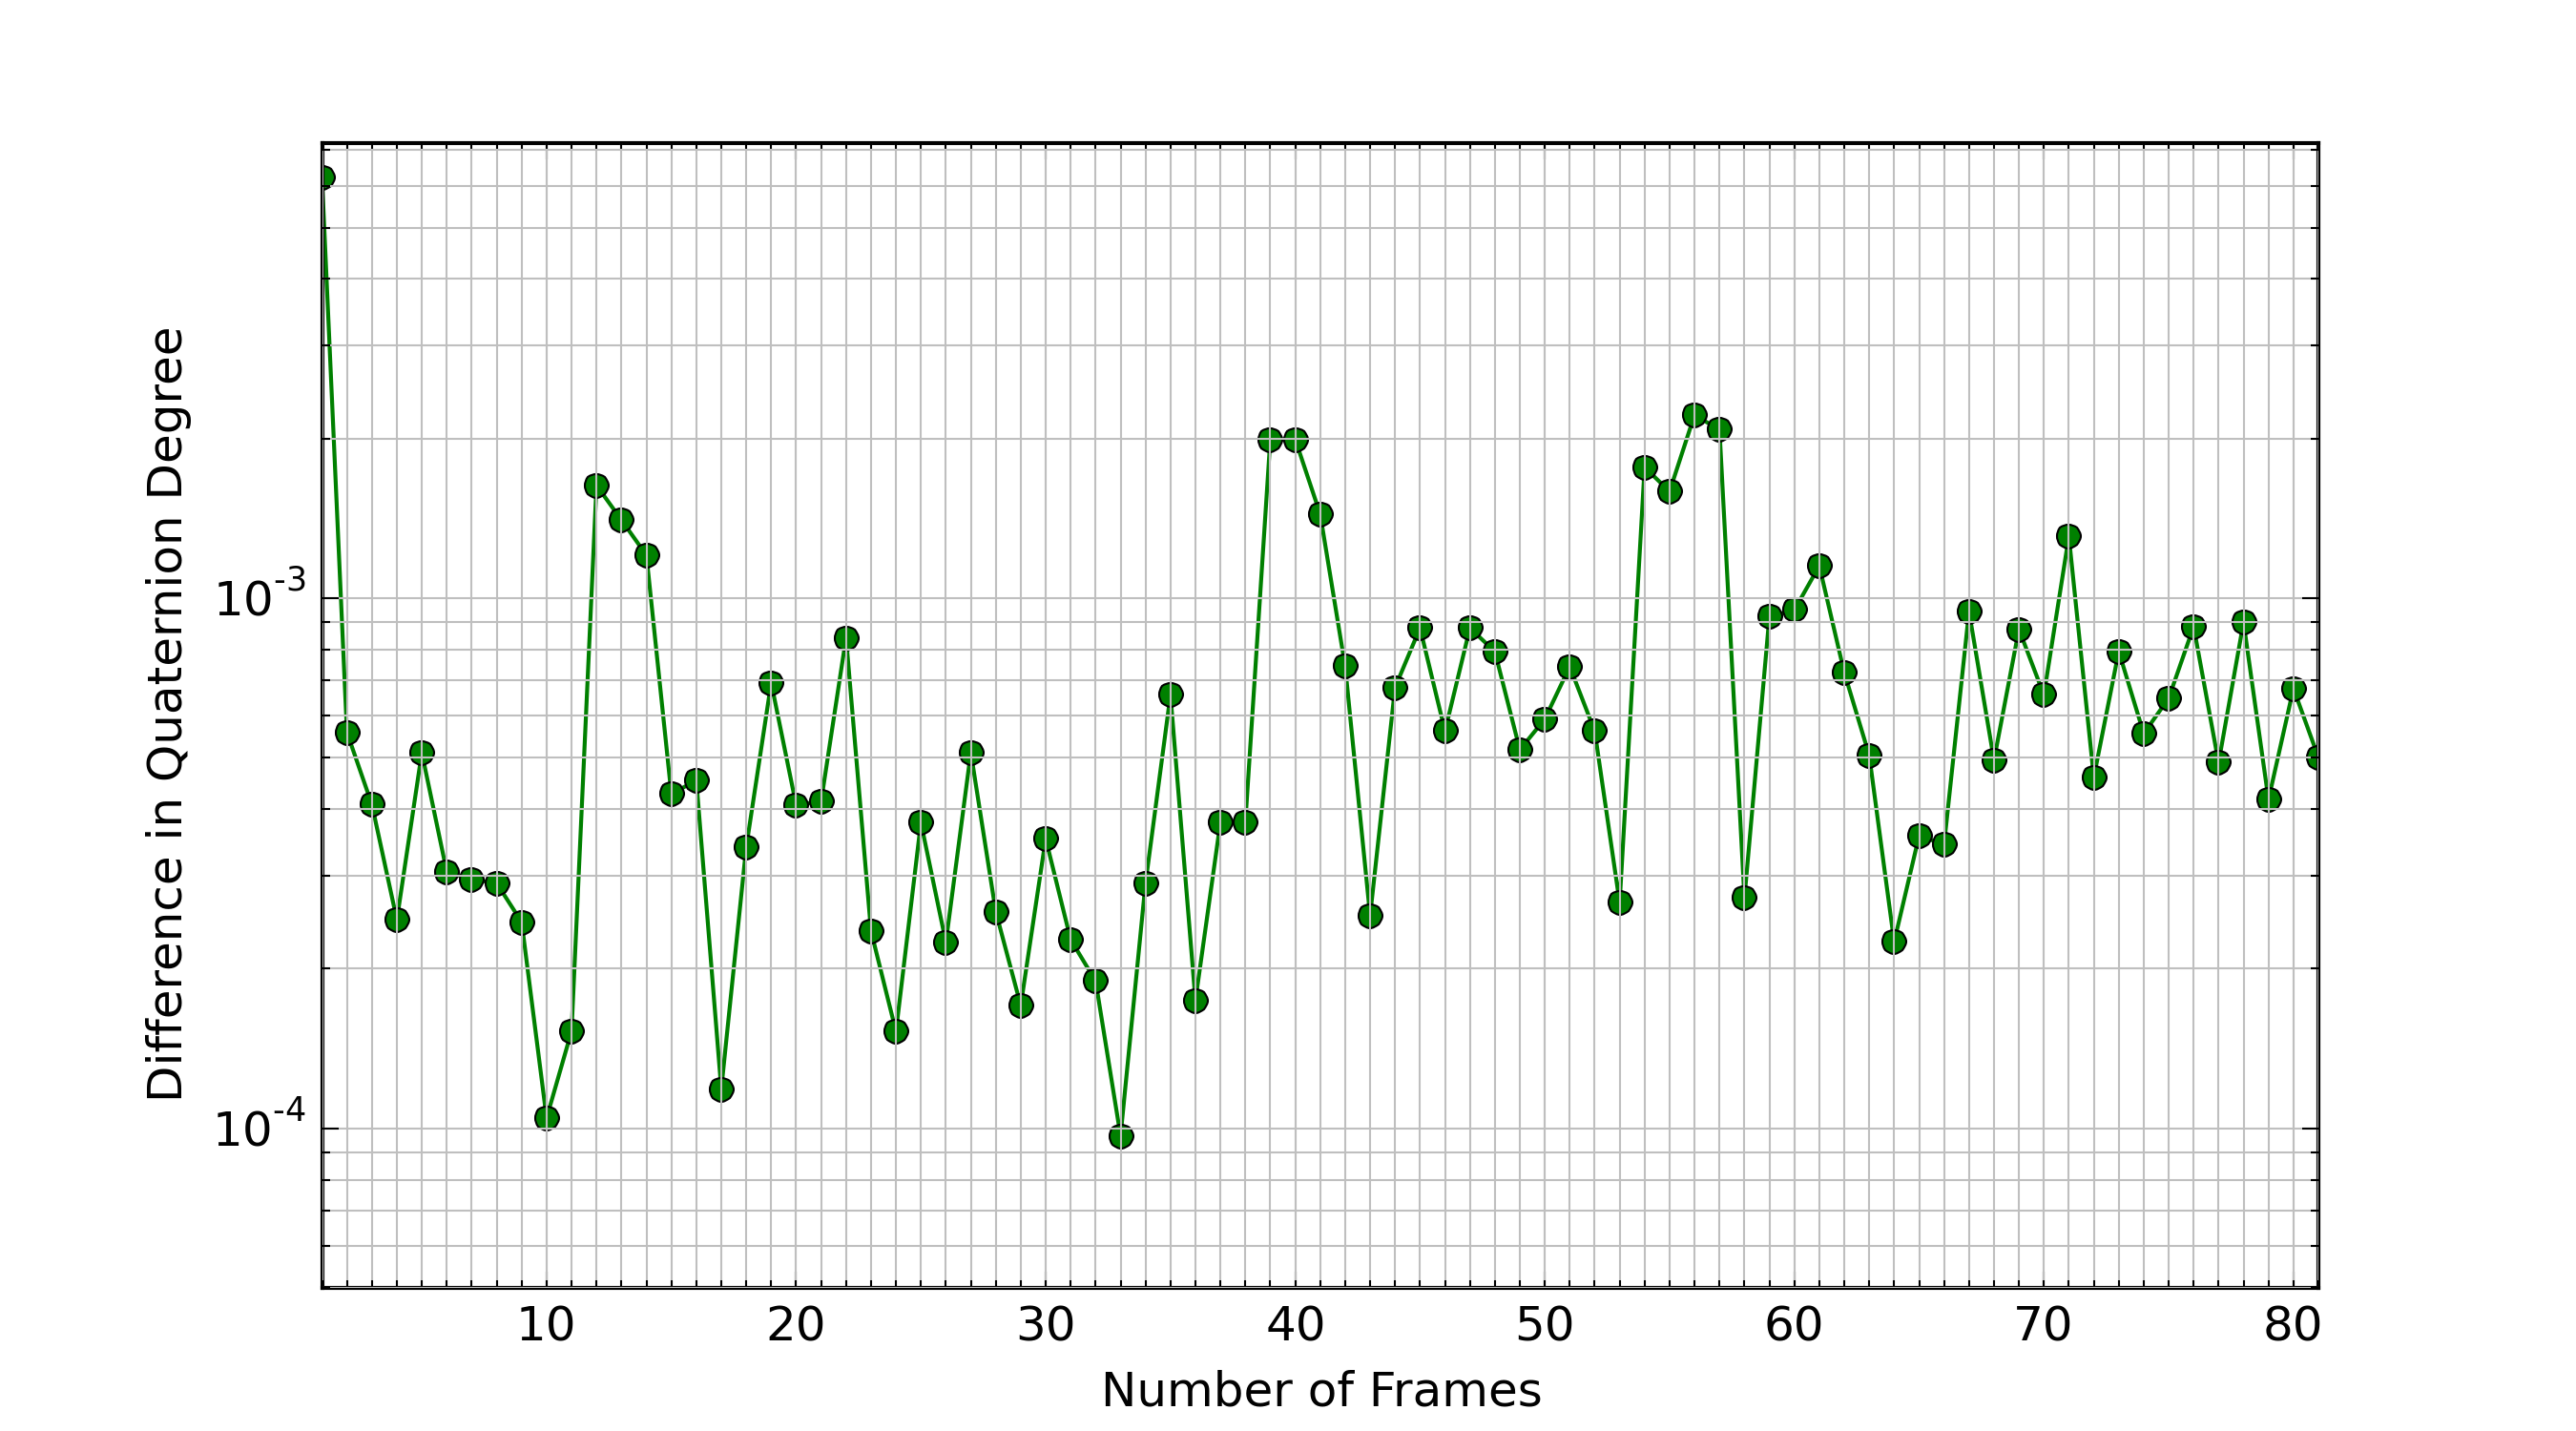
\includegraphics[width=80mm]{figures/diff_600/graph_rotation} \\
(a) difference of translation in milliliters & (b) difference of rotation in degree of quaternion \\[6pt]
\end{tabular}
\caption{The difference between the Feature-based and Marker-based for each sequence pair of third sample data set}\label{fig:sample_03_diff}
\end{figure}

\begin{table}[H]
\centering
  \begin{tabular}{| c | c | c | c |}
      \hline
      \multicolumn{2}{|c|}{Translation} & \multicolumn{2}{c}{Rotation} \\ \hline
       Mean & Standard Deviation & Mean & Standard Deviation \\ \hline
      0.6558 & 1.4589 & 0.0007 & 0.0008 \\ \hline
  \end{tabular}
  \caption{} \label{tab:sample_03_diff}
\end{table}

\section{Test Local Threshold} \label{sec:local_threshold}
In this test, we evaluate the performance of a parameter that describes the number of images in a bundle. This size is called local threshold. In this test we run the first sample data set (\autoref{sec:sample_01}) for three times with the size of 3, 5, and 7 for a bundle.
\begin{figure}[H]
\centering
\begin{tabular}{cc}
  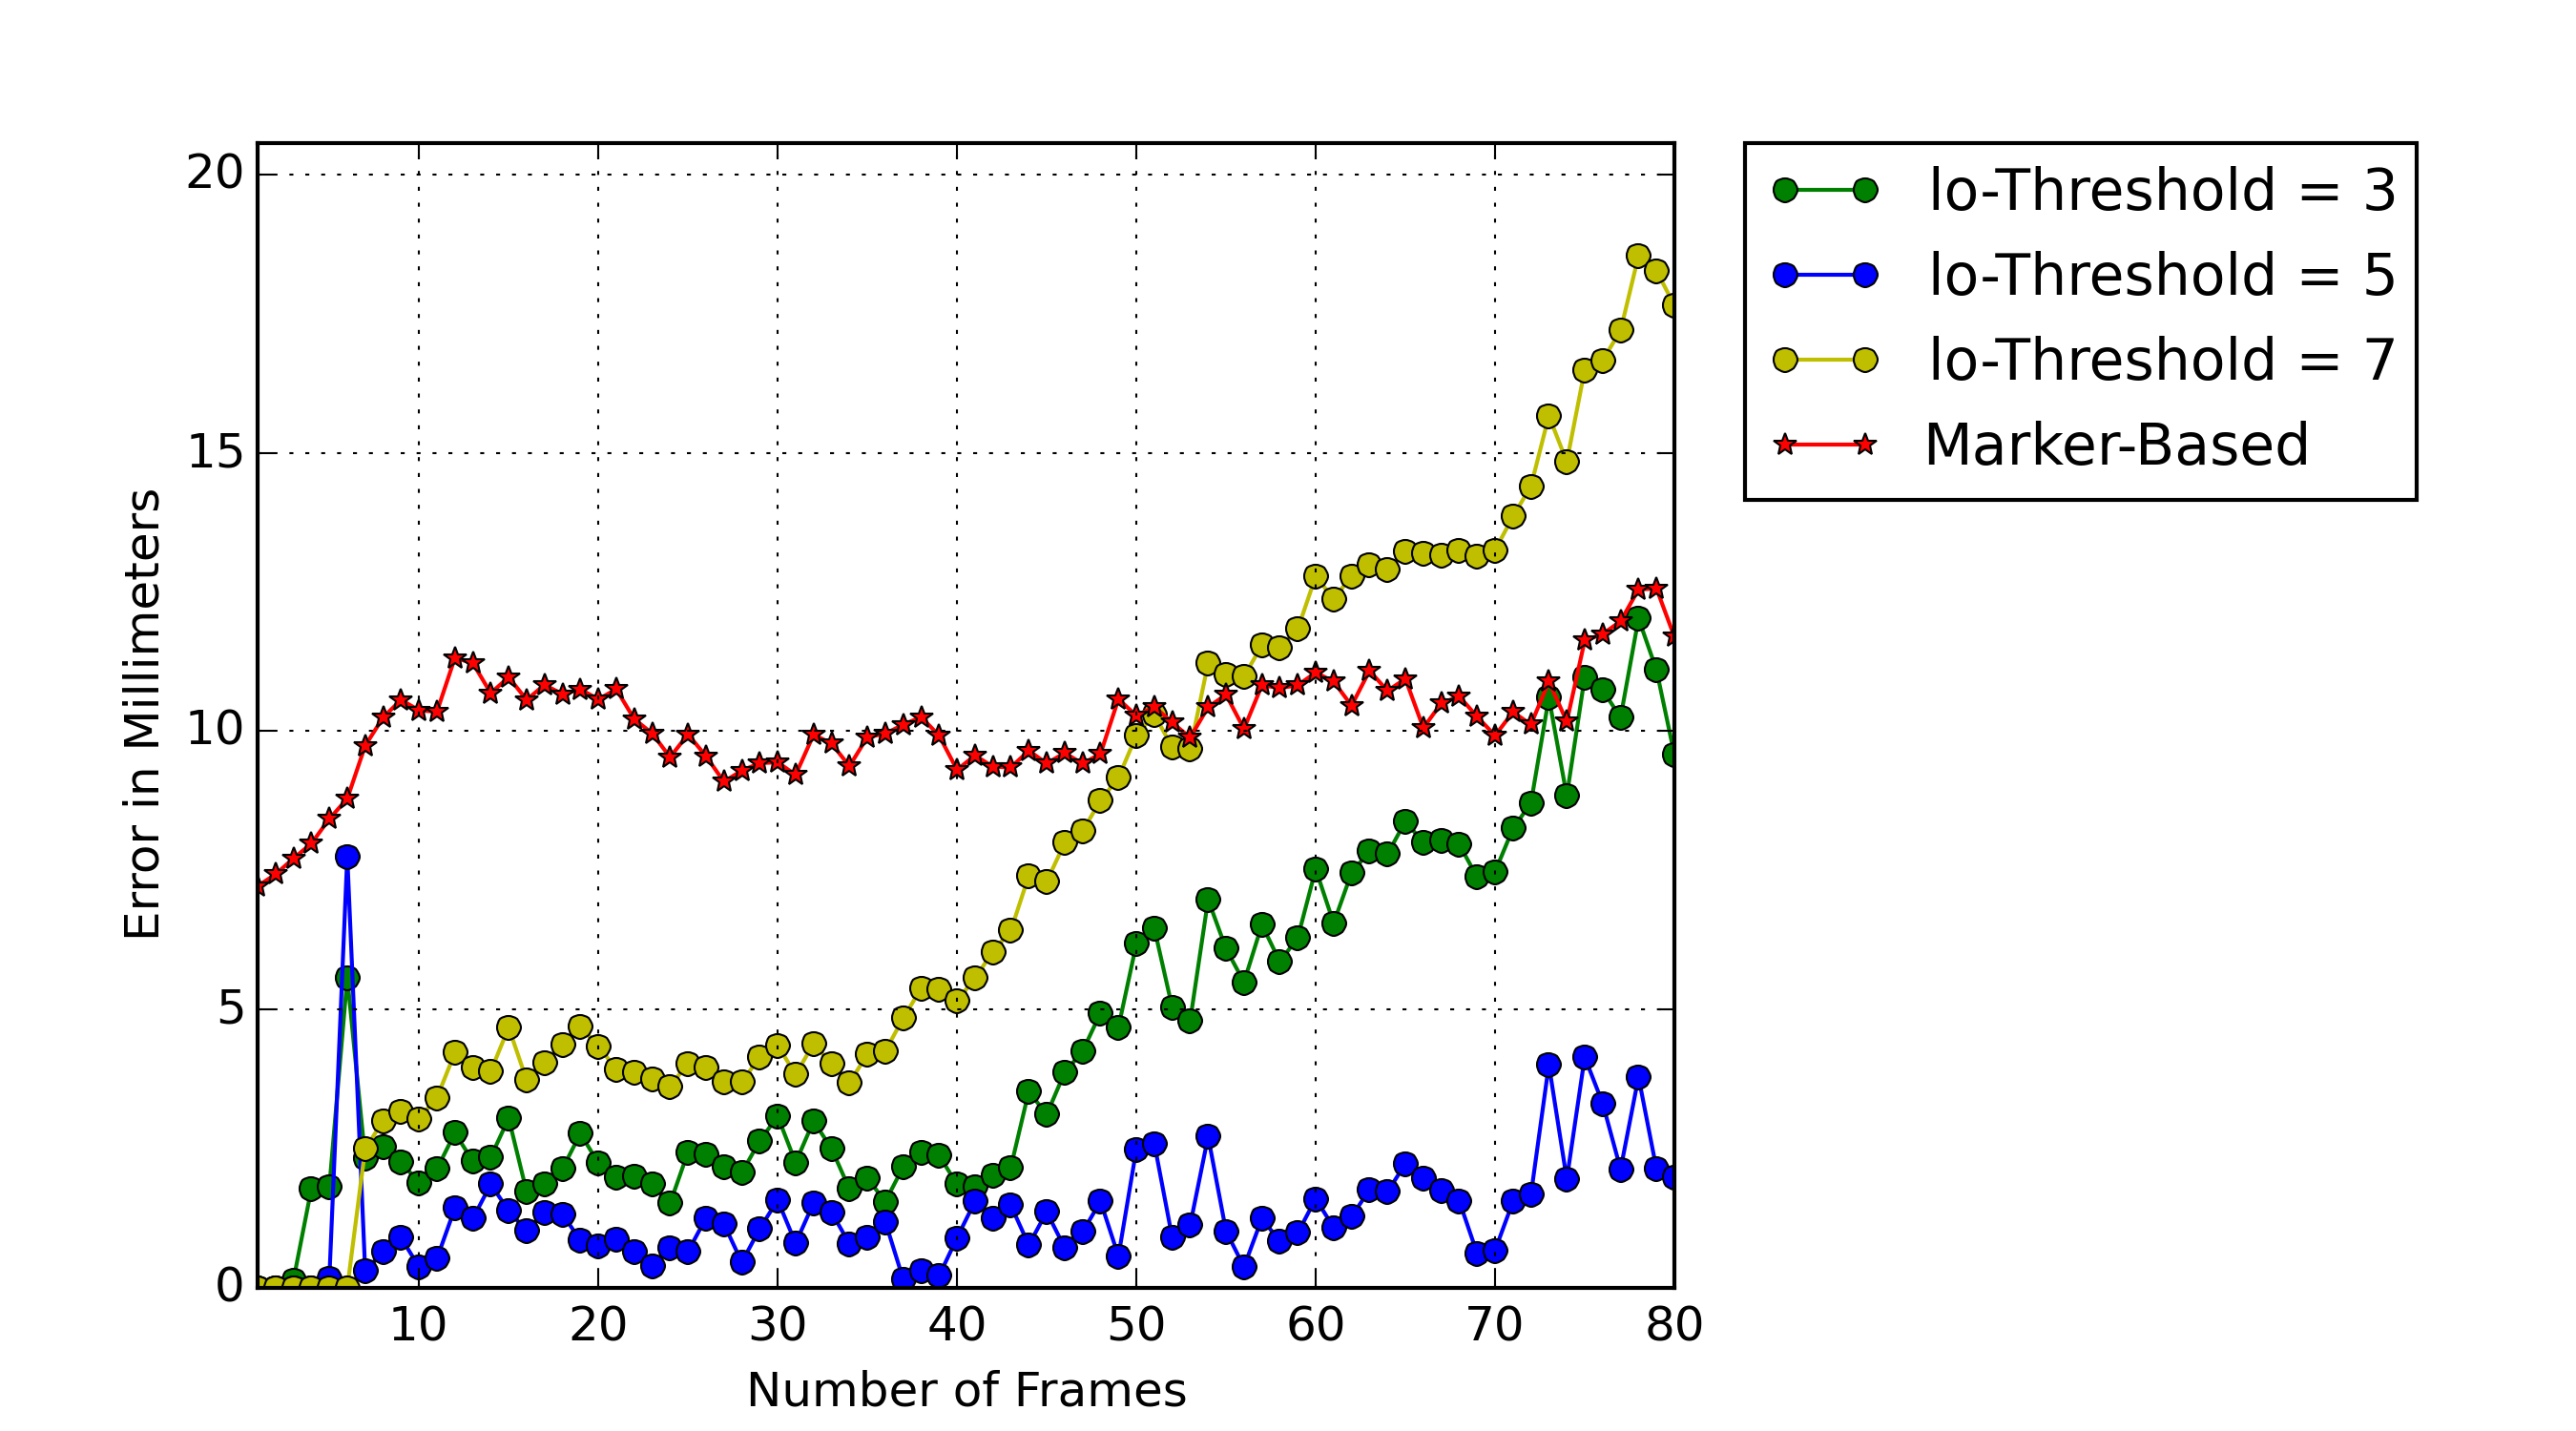
\includegraphics[width=80mm]{figures/local/graph_translation} &   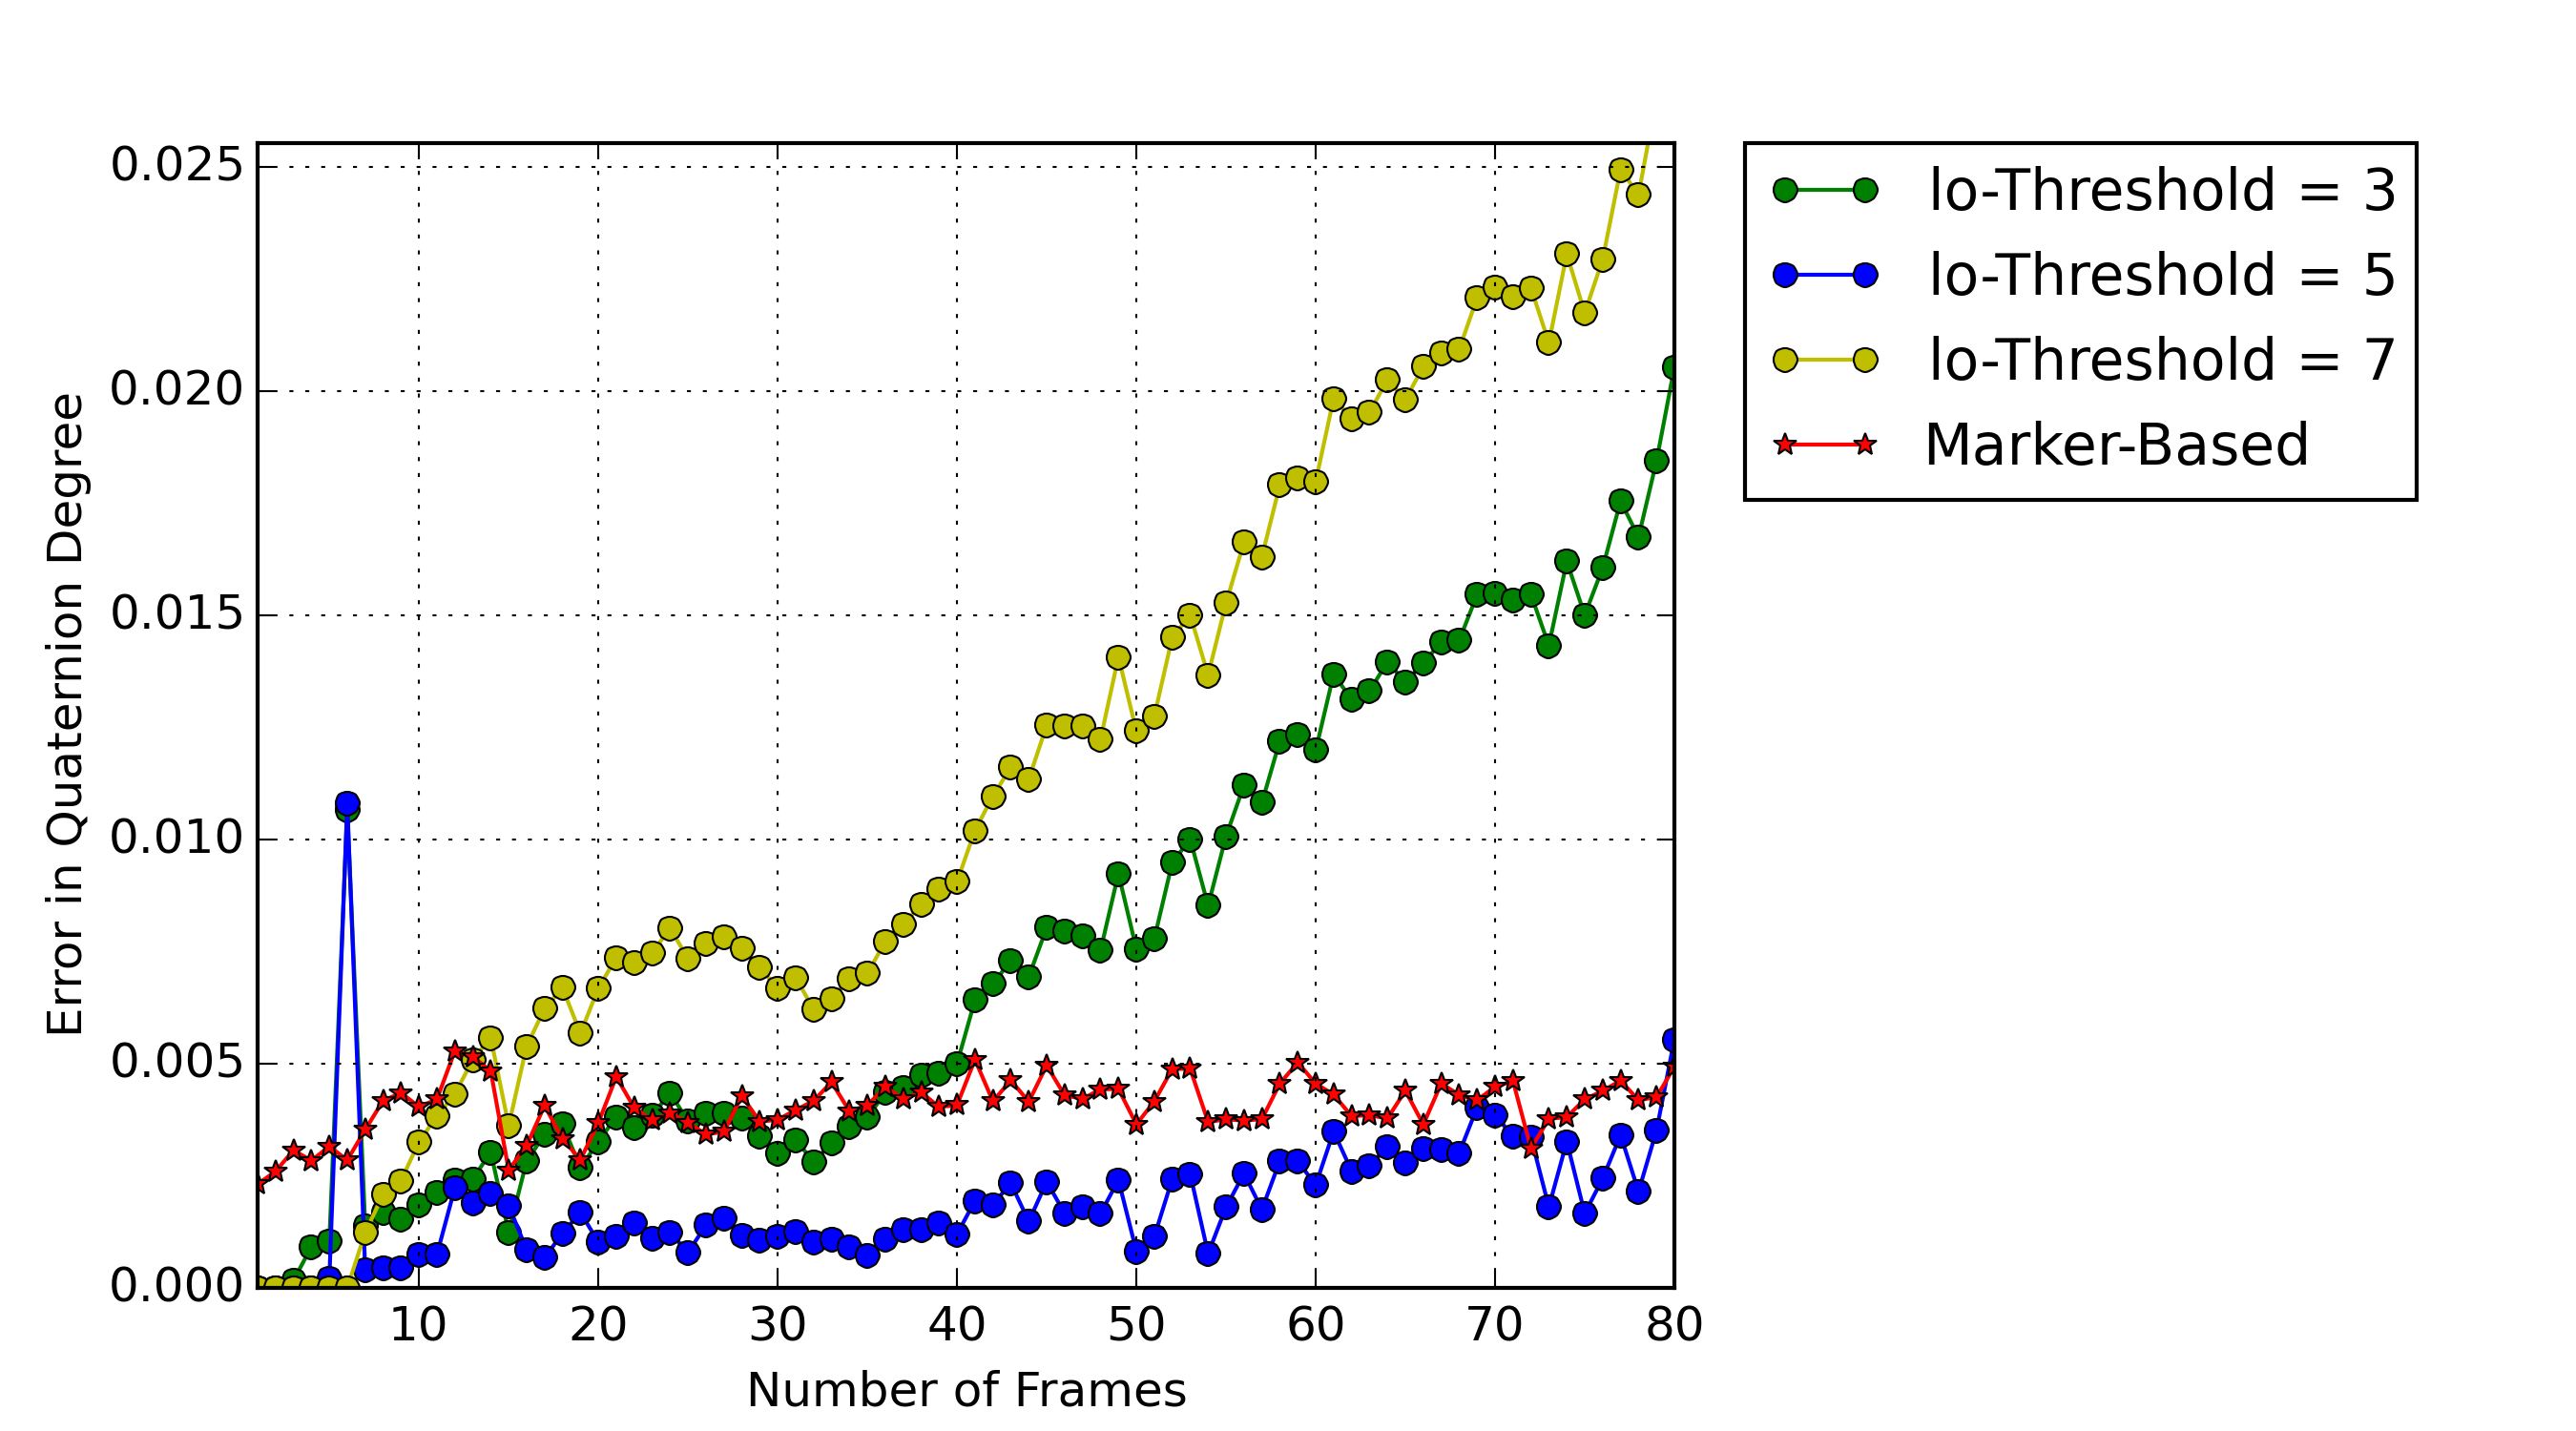
\includegraphics[width=80mm]{figures/local/graph_rotation}  \\
  the translation error & the rotation error \\[6pt]
\end{tabular}
\caption{The translation and rotation error for marker-based Ubitrack method and feature-based with a variety of values for local threshold}\label{fig:test_local_threshold}
\end{figure}

\begin{table}[H]
\centering
  \begin{tabular}{| c || c | c | c | c |}
      \hline
      & \multicolumn{2}{c|}{Translation} & \multicolumn{2}{c|}{Rotation} \\ \hline
       & Mean & Standard Deviation & Mean & Standard Deviation \\ \hline
      local threshold = 3 & 4.5165 & 3.0451 & 0.0076 & 0.0054 \\ \hline
      local threshold = 5 & \textbf{1.3303} & 1.1184 & \textbf{0.0019} & 0.0015 \\ \hline
      local threshold = 7 & 7.7309 & 5.0268 & 0.0117 & 0.0075 \\ \hline
      Marker-based Ubitrack & 10.1552 & \textbf{0.9700} & 0.0040 & \textbf{0.0006} \\ \hline
  \end{tabular}
  \caption{The statistical analysis of feature-based with different values for local threshold} \label{tab:test_local_threshold}
\end{table}

It is clear that for the both translation and rotation tests, the local threshold with size 5 is winner where the mean of translation is 1.3303 millimeters and for the rotation is 0.0019 degree of quaternion. After that, for the rotation case, the Ubitrack marker-based approach is located in the second place whereas for the translation, the local threshold with size 3 with average 4.5165 is set as the second best candidate. It is noticeable that for the both translations and rotation the Ubitrack marker-based method has the lowest standard deviation among the all methods.

\section{Test Global Threshold} \label{sec:global_threshold}
The next Threshold in our approach is about the number of frames that we process for the global bundle adjustment and updating the 3D points in world map vector. After each global threshold, The 3D points in world map completely replace with the new data. more information was explained in \autoref{subsec:update_3d_points}.
\begin{figure}[H]
\centering
\begin{tabular}{cc}
  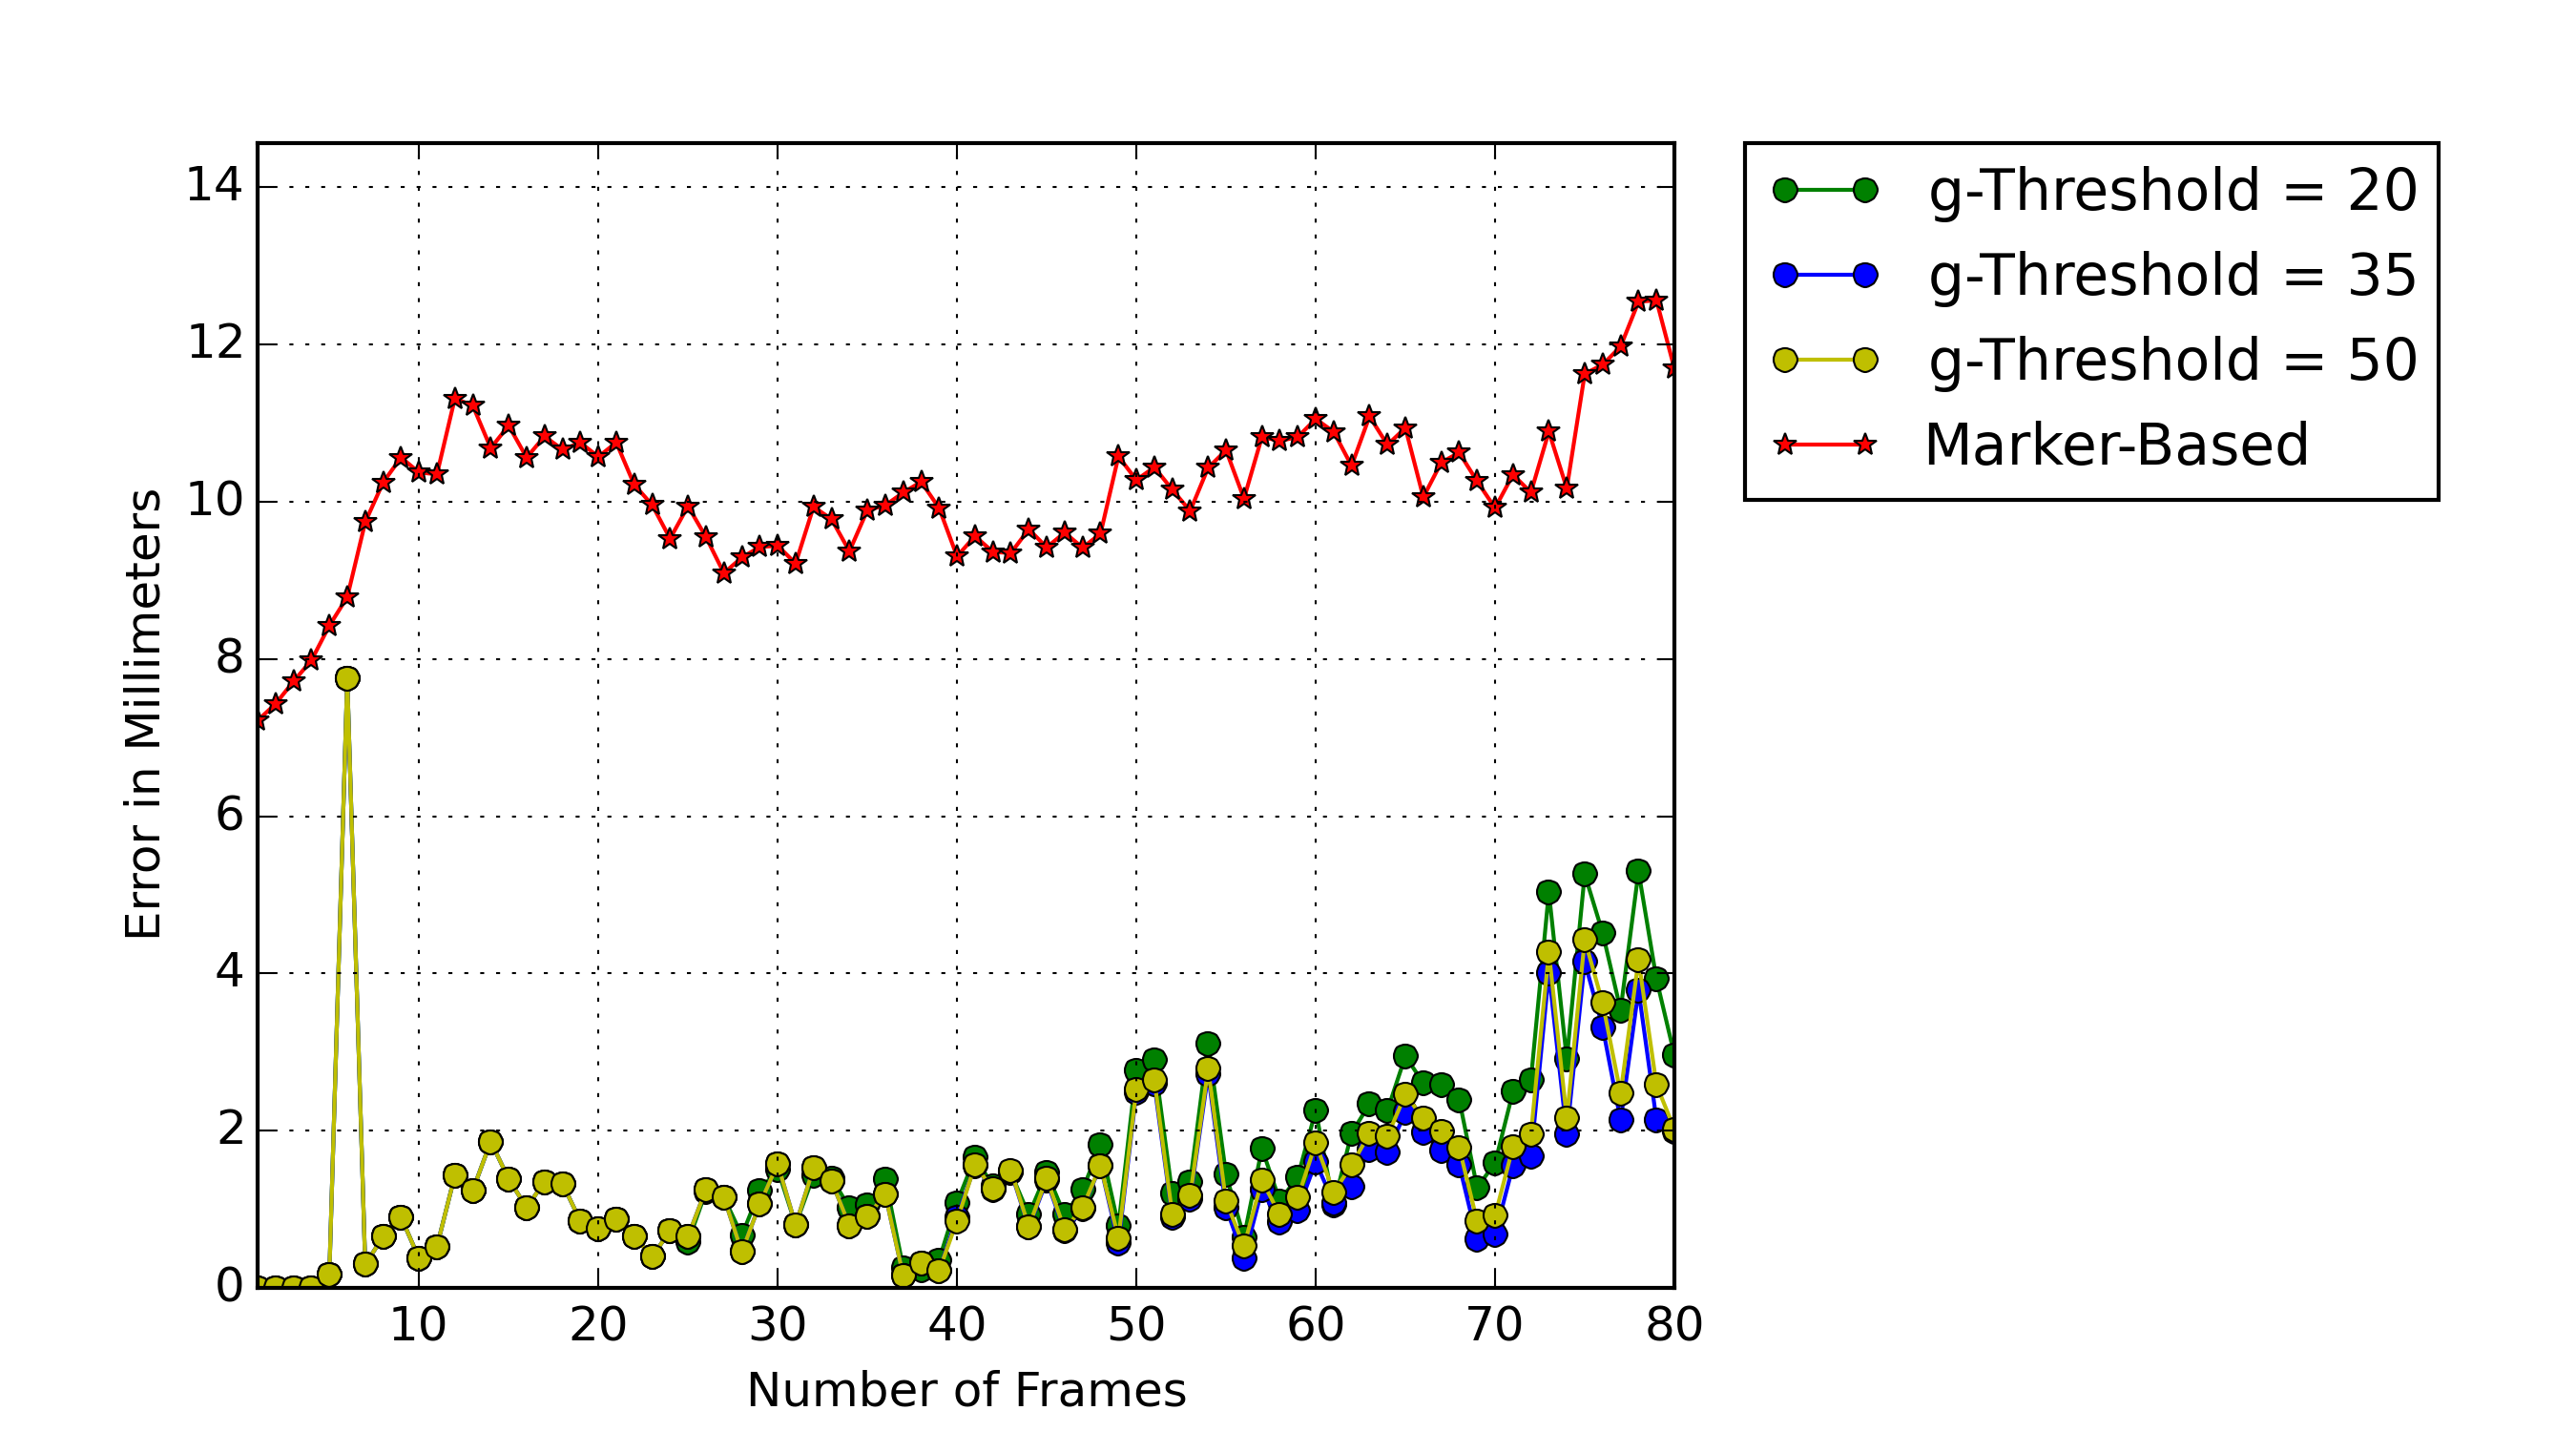
\includegraphics[width=80mm]{figures/global/graph_translation} &   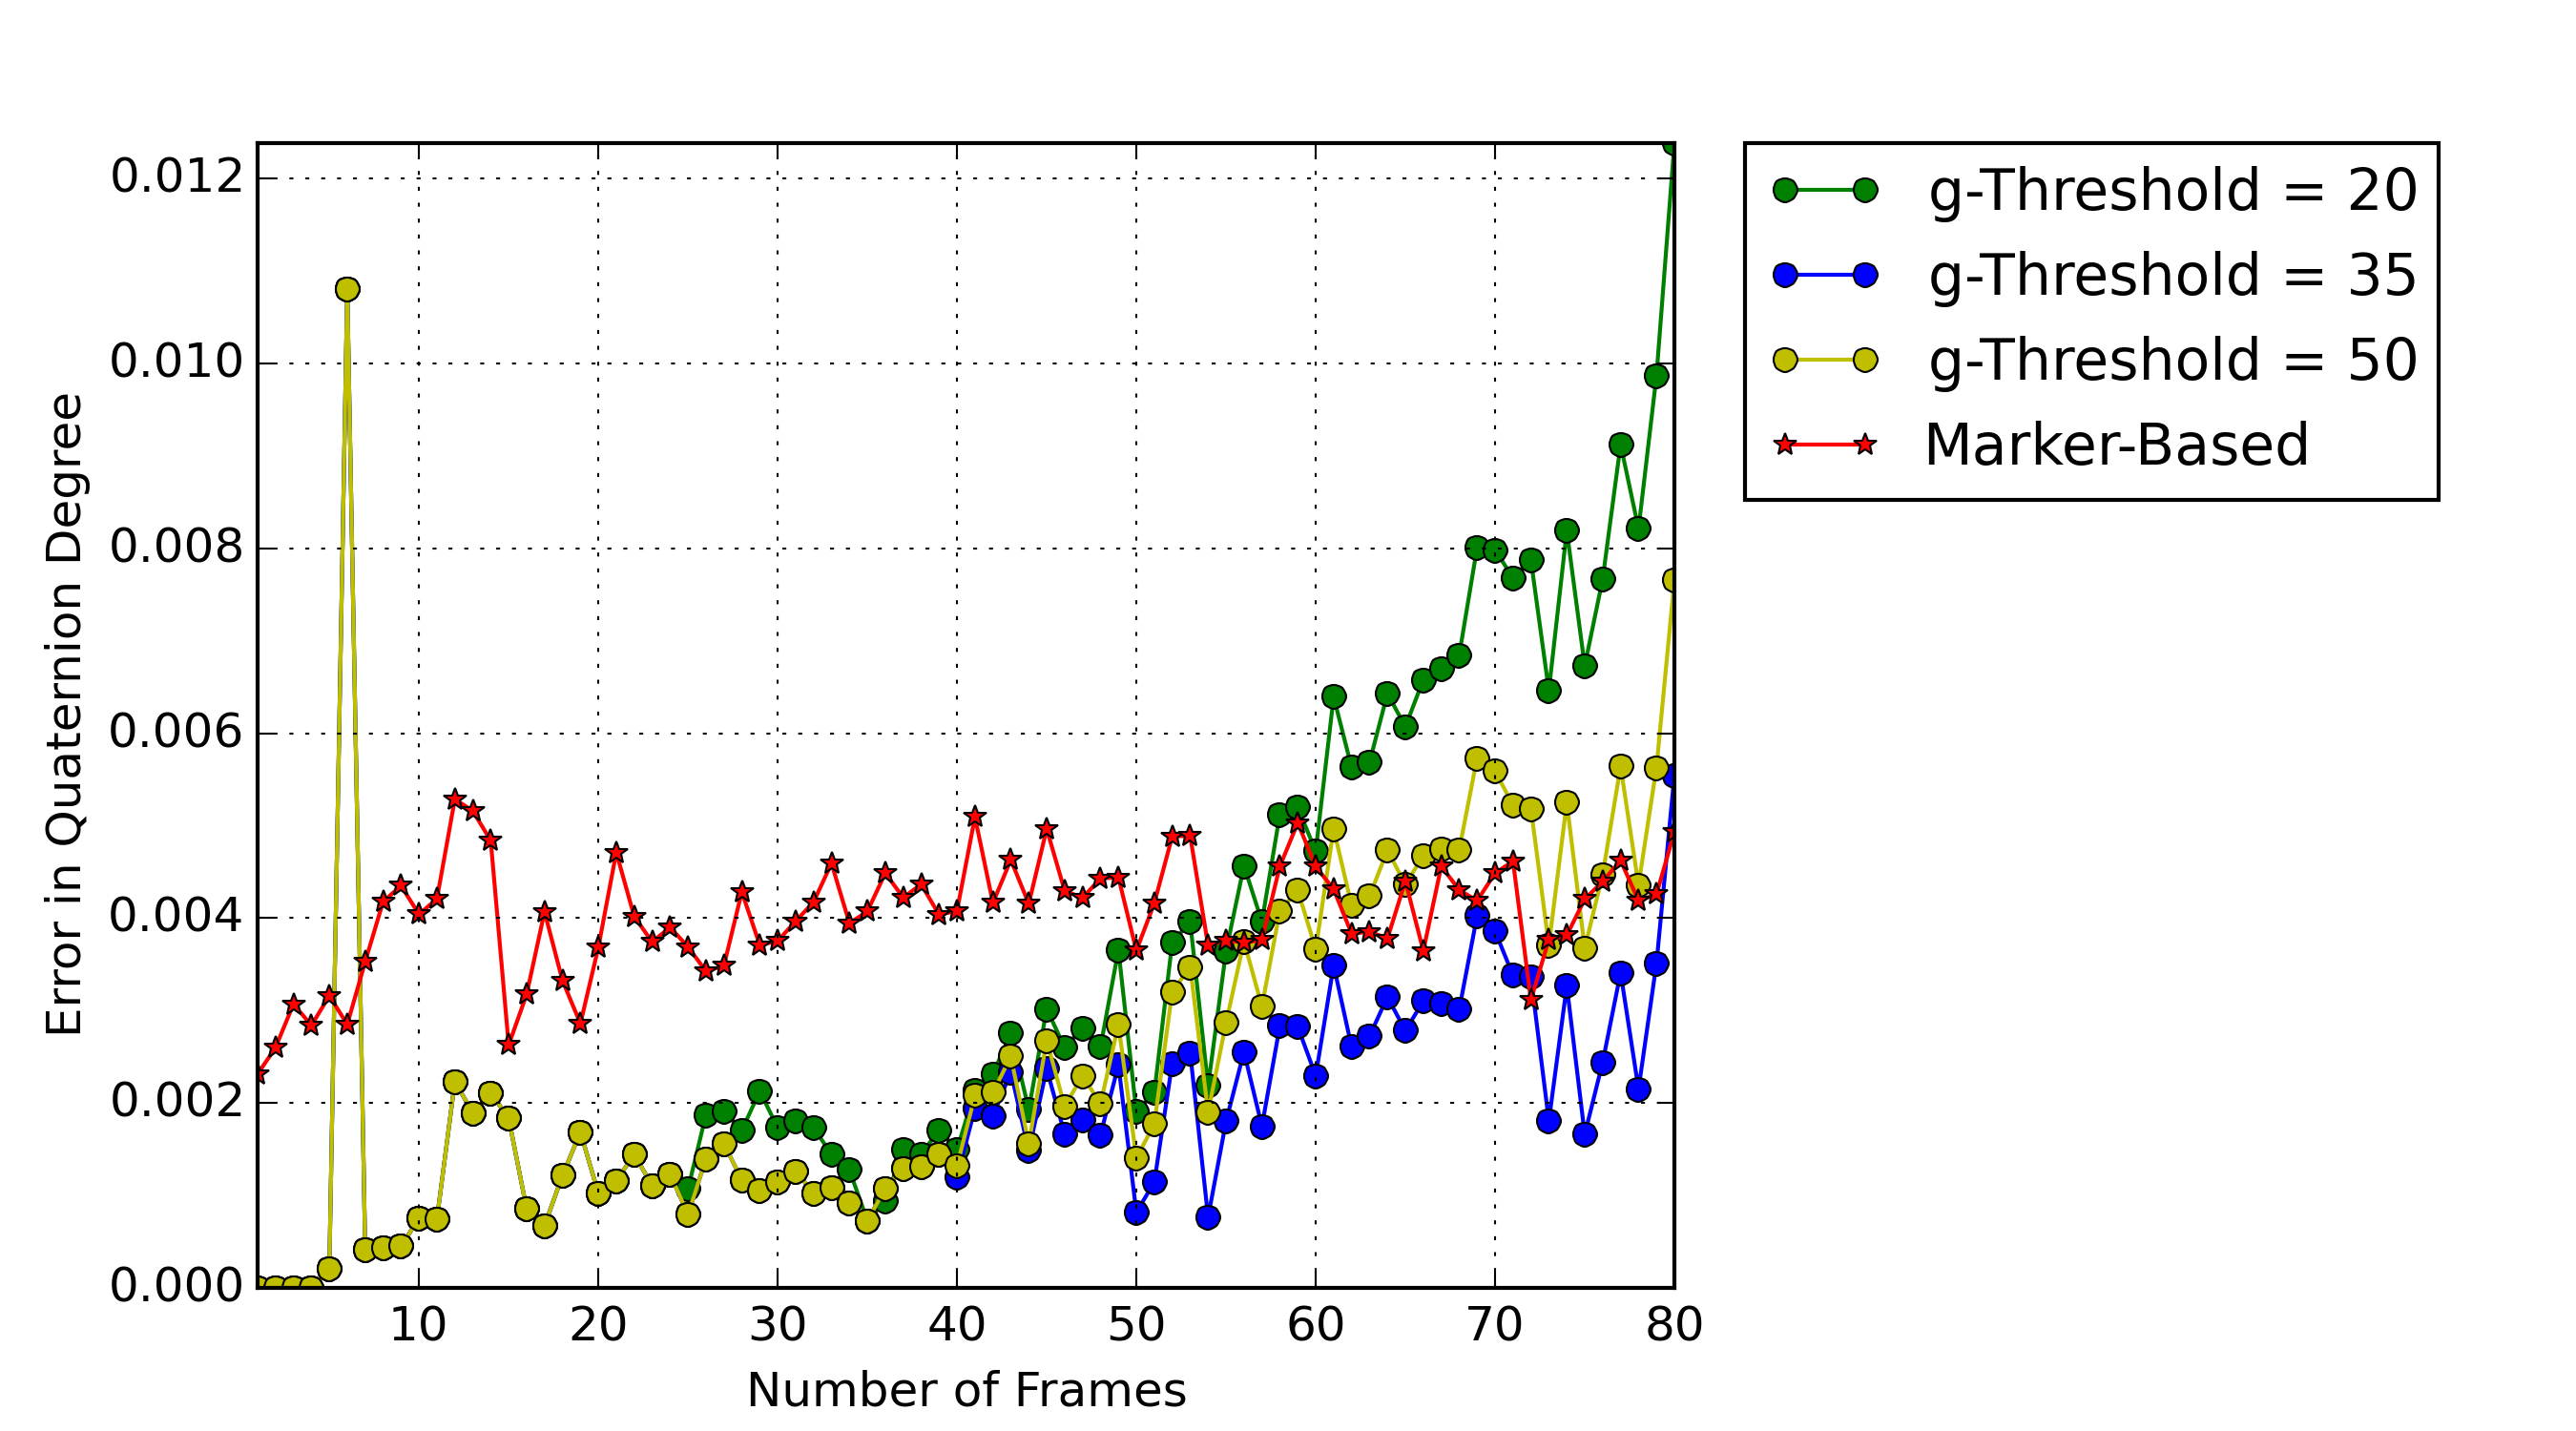
\includegraphics[width=80mm]{figures/global/graph_rotation}  \\
  the translation error & the rotation error \\[6pt]
\end{tabular}
\caption{}\label{fig:test_global_threshold}

\end{figure}
\begin{table}[H]
\centering
  \begin{tabular}{| c || c | c | c | c |}
      \hline
      & \multicolumn{2}{c|}{Translation} & \multicolumn{2}{c|}{Rotation} \\ \hline
       & Mean & Standard Deviation & Mean & Standard Deviation \\ \hline
      global threshold = 20 & 1.6392 & 1.3589 & 0.0034 & 0.0029 \\ \hline
      global threshold = 35 & \textbf{1.3303} & 1.1184 & \textbf{0.0019} & 0.0015 \\ \hline
      global threshold = 50 & 1.4071 & 1.1697 & 0.0025 & 0.0020 \\ \hline
      Marker-based Ubitrack & 10.1552 & \textbf{0.9700} & 0.0040 & \textbf{0.0006} \\ \hline
  \end{tabular}
  \caption{The statistical analysis of feature-based with different values for global threshold} \label{tab:test_global_threshold}
\end{table}
The result of global threshold for all cases 20, 35 and 50 are mostly close together. In fact, the result of all values for tracking are same whereas the result of global threshold 35 has the best result for rotation. In this test also the Ubitrack has the lowest standard deviation among all methods that were tested.

\section{Reference System} \label{sec:refrence_system}
In the last test, we evaluate the performance of a system in which its reference camera poses are taken from ARTrack for the all frames of first bundle compare to the systems that are computed by the planer tracking with the homography matrix.
\begin{figure}[H]
\begin{tabular}{cc}
  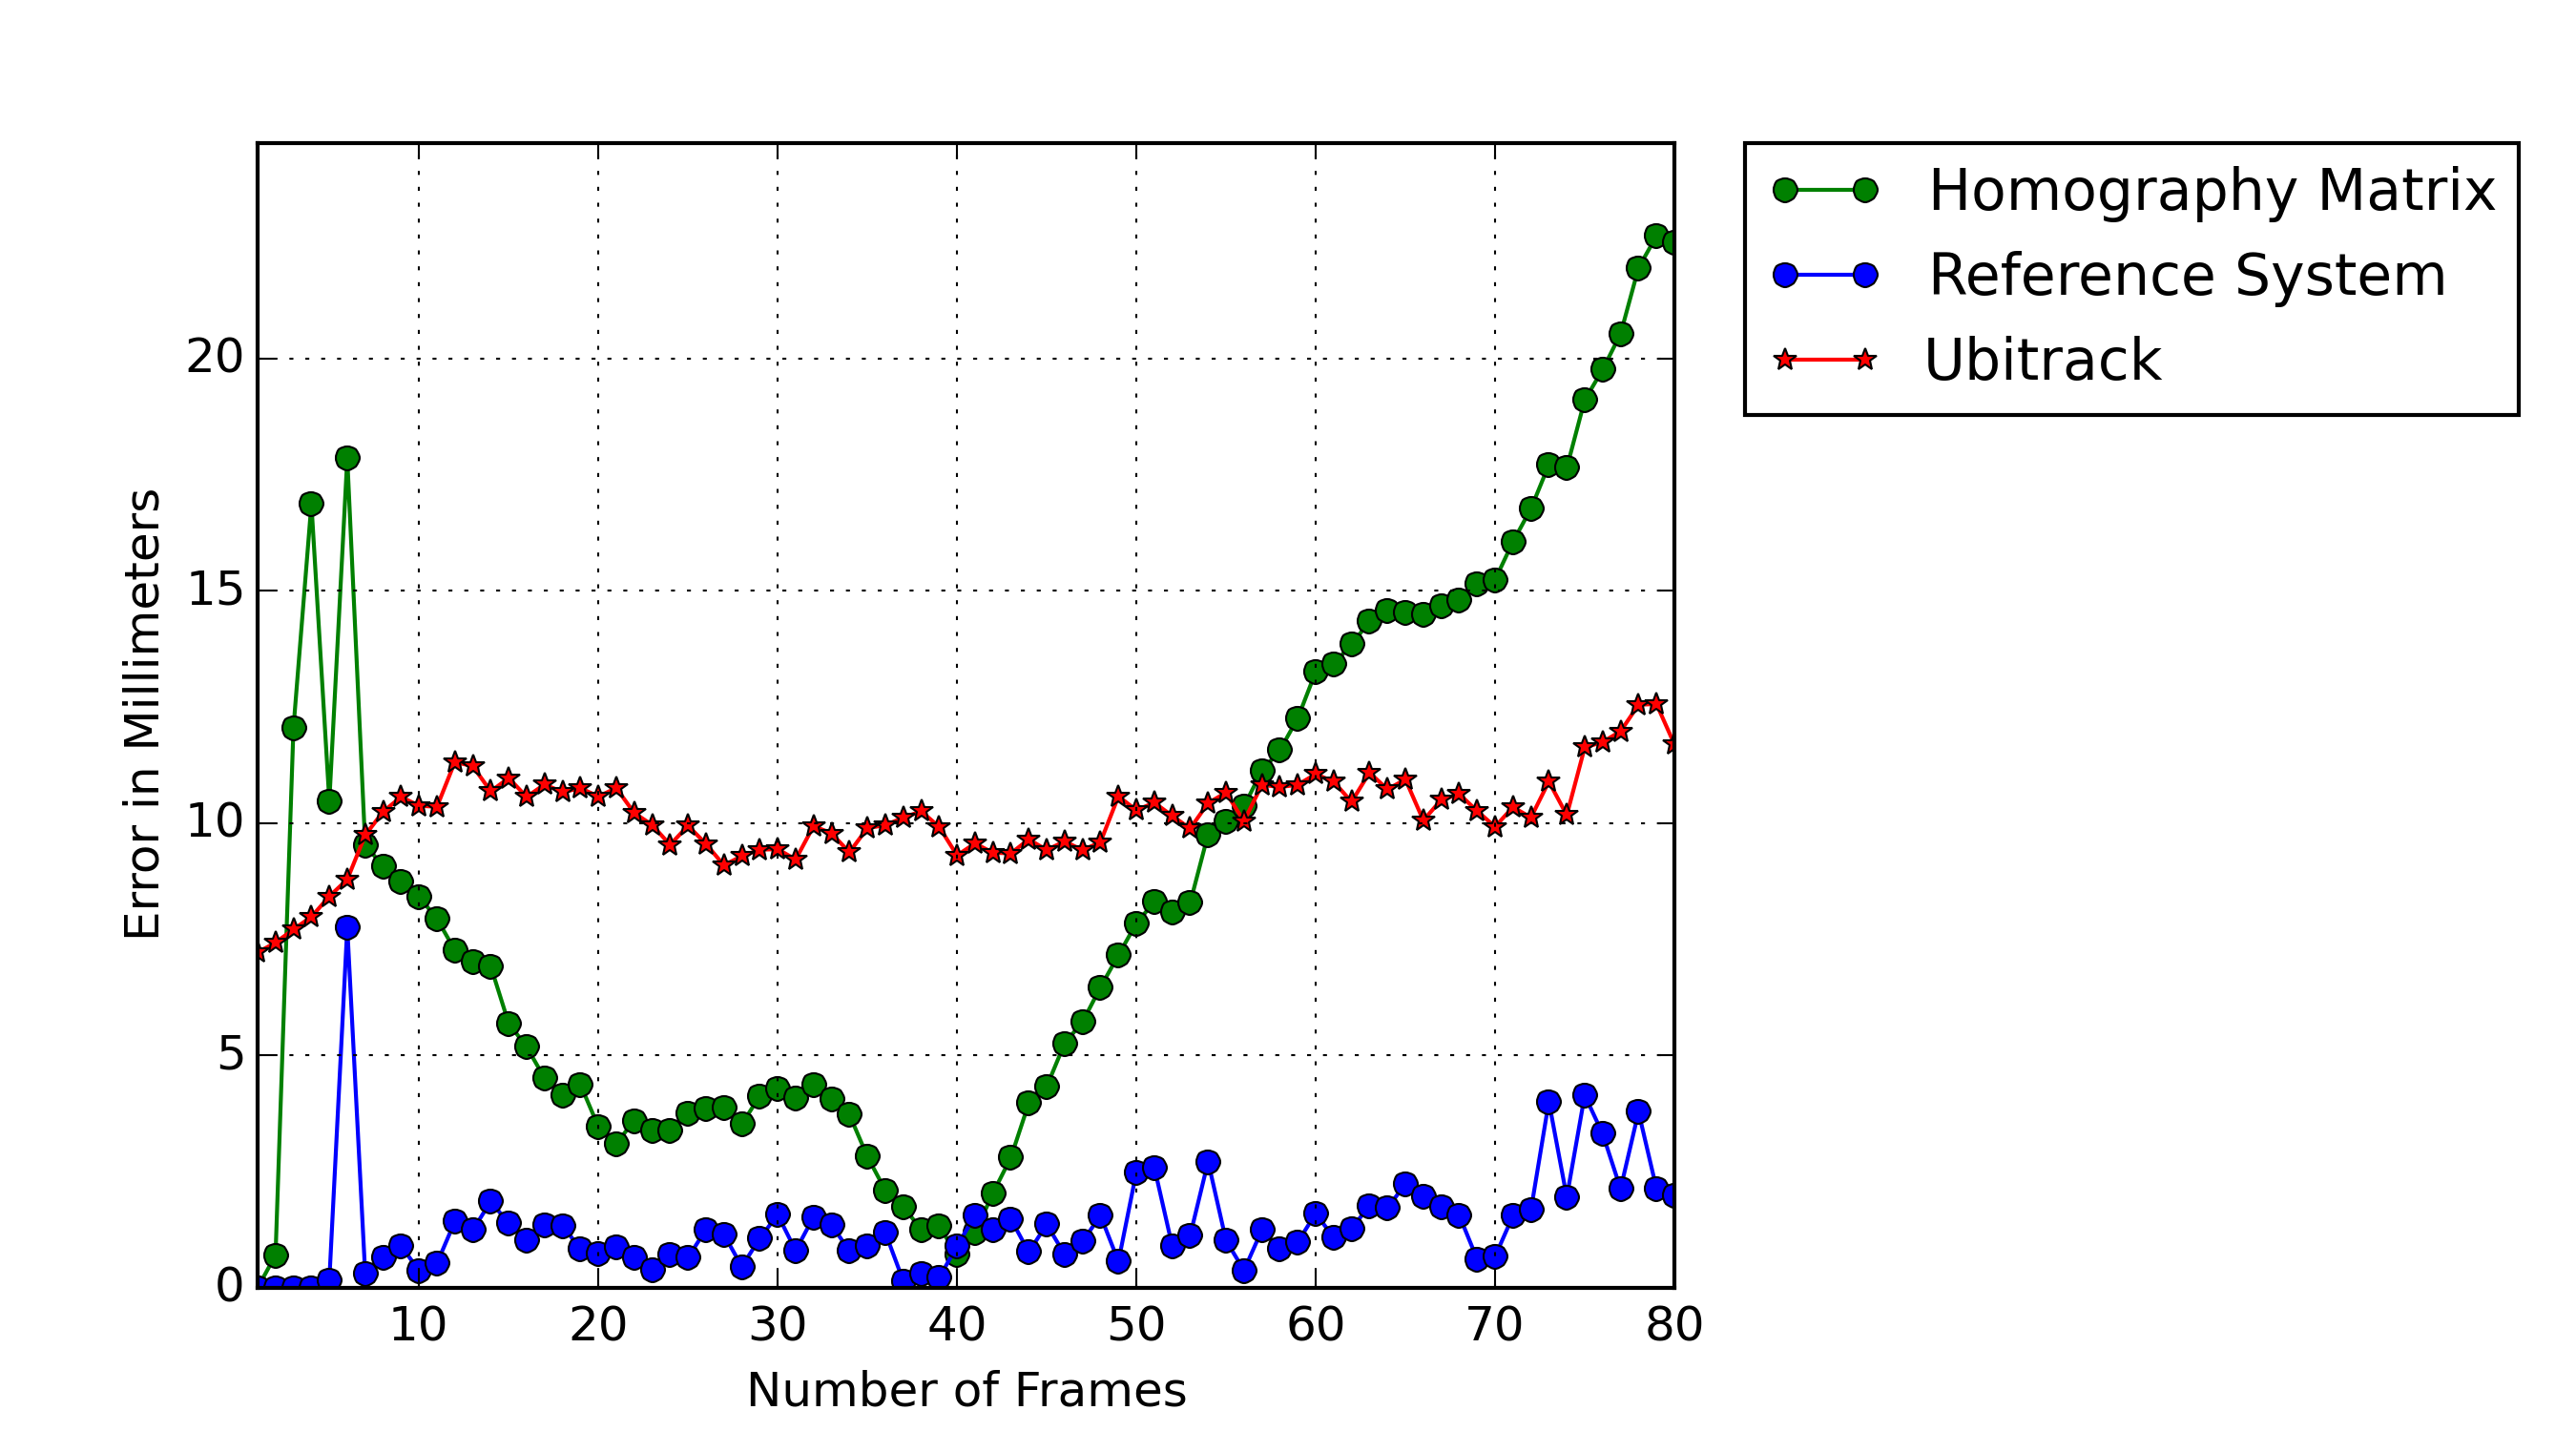
\includegraphics[width=80mm]{figures/homo/graph_translation} &  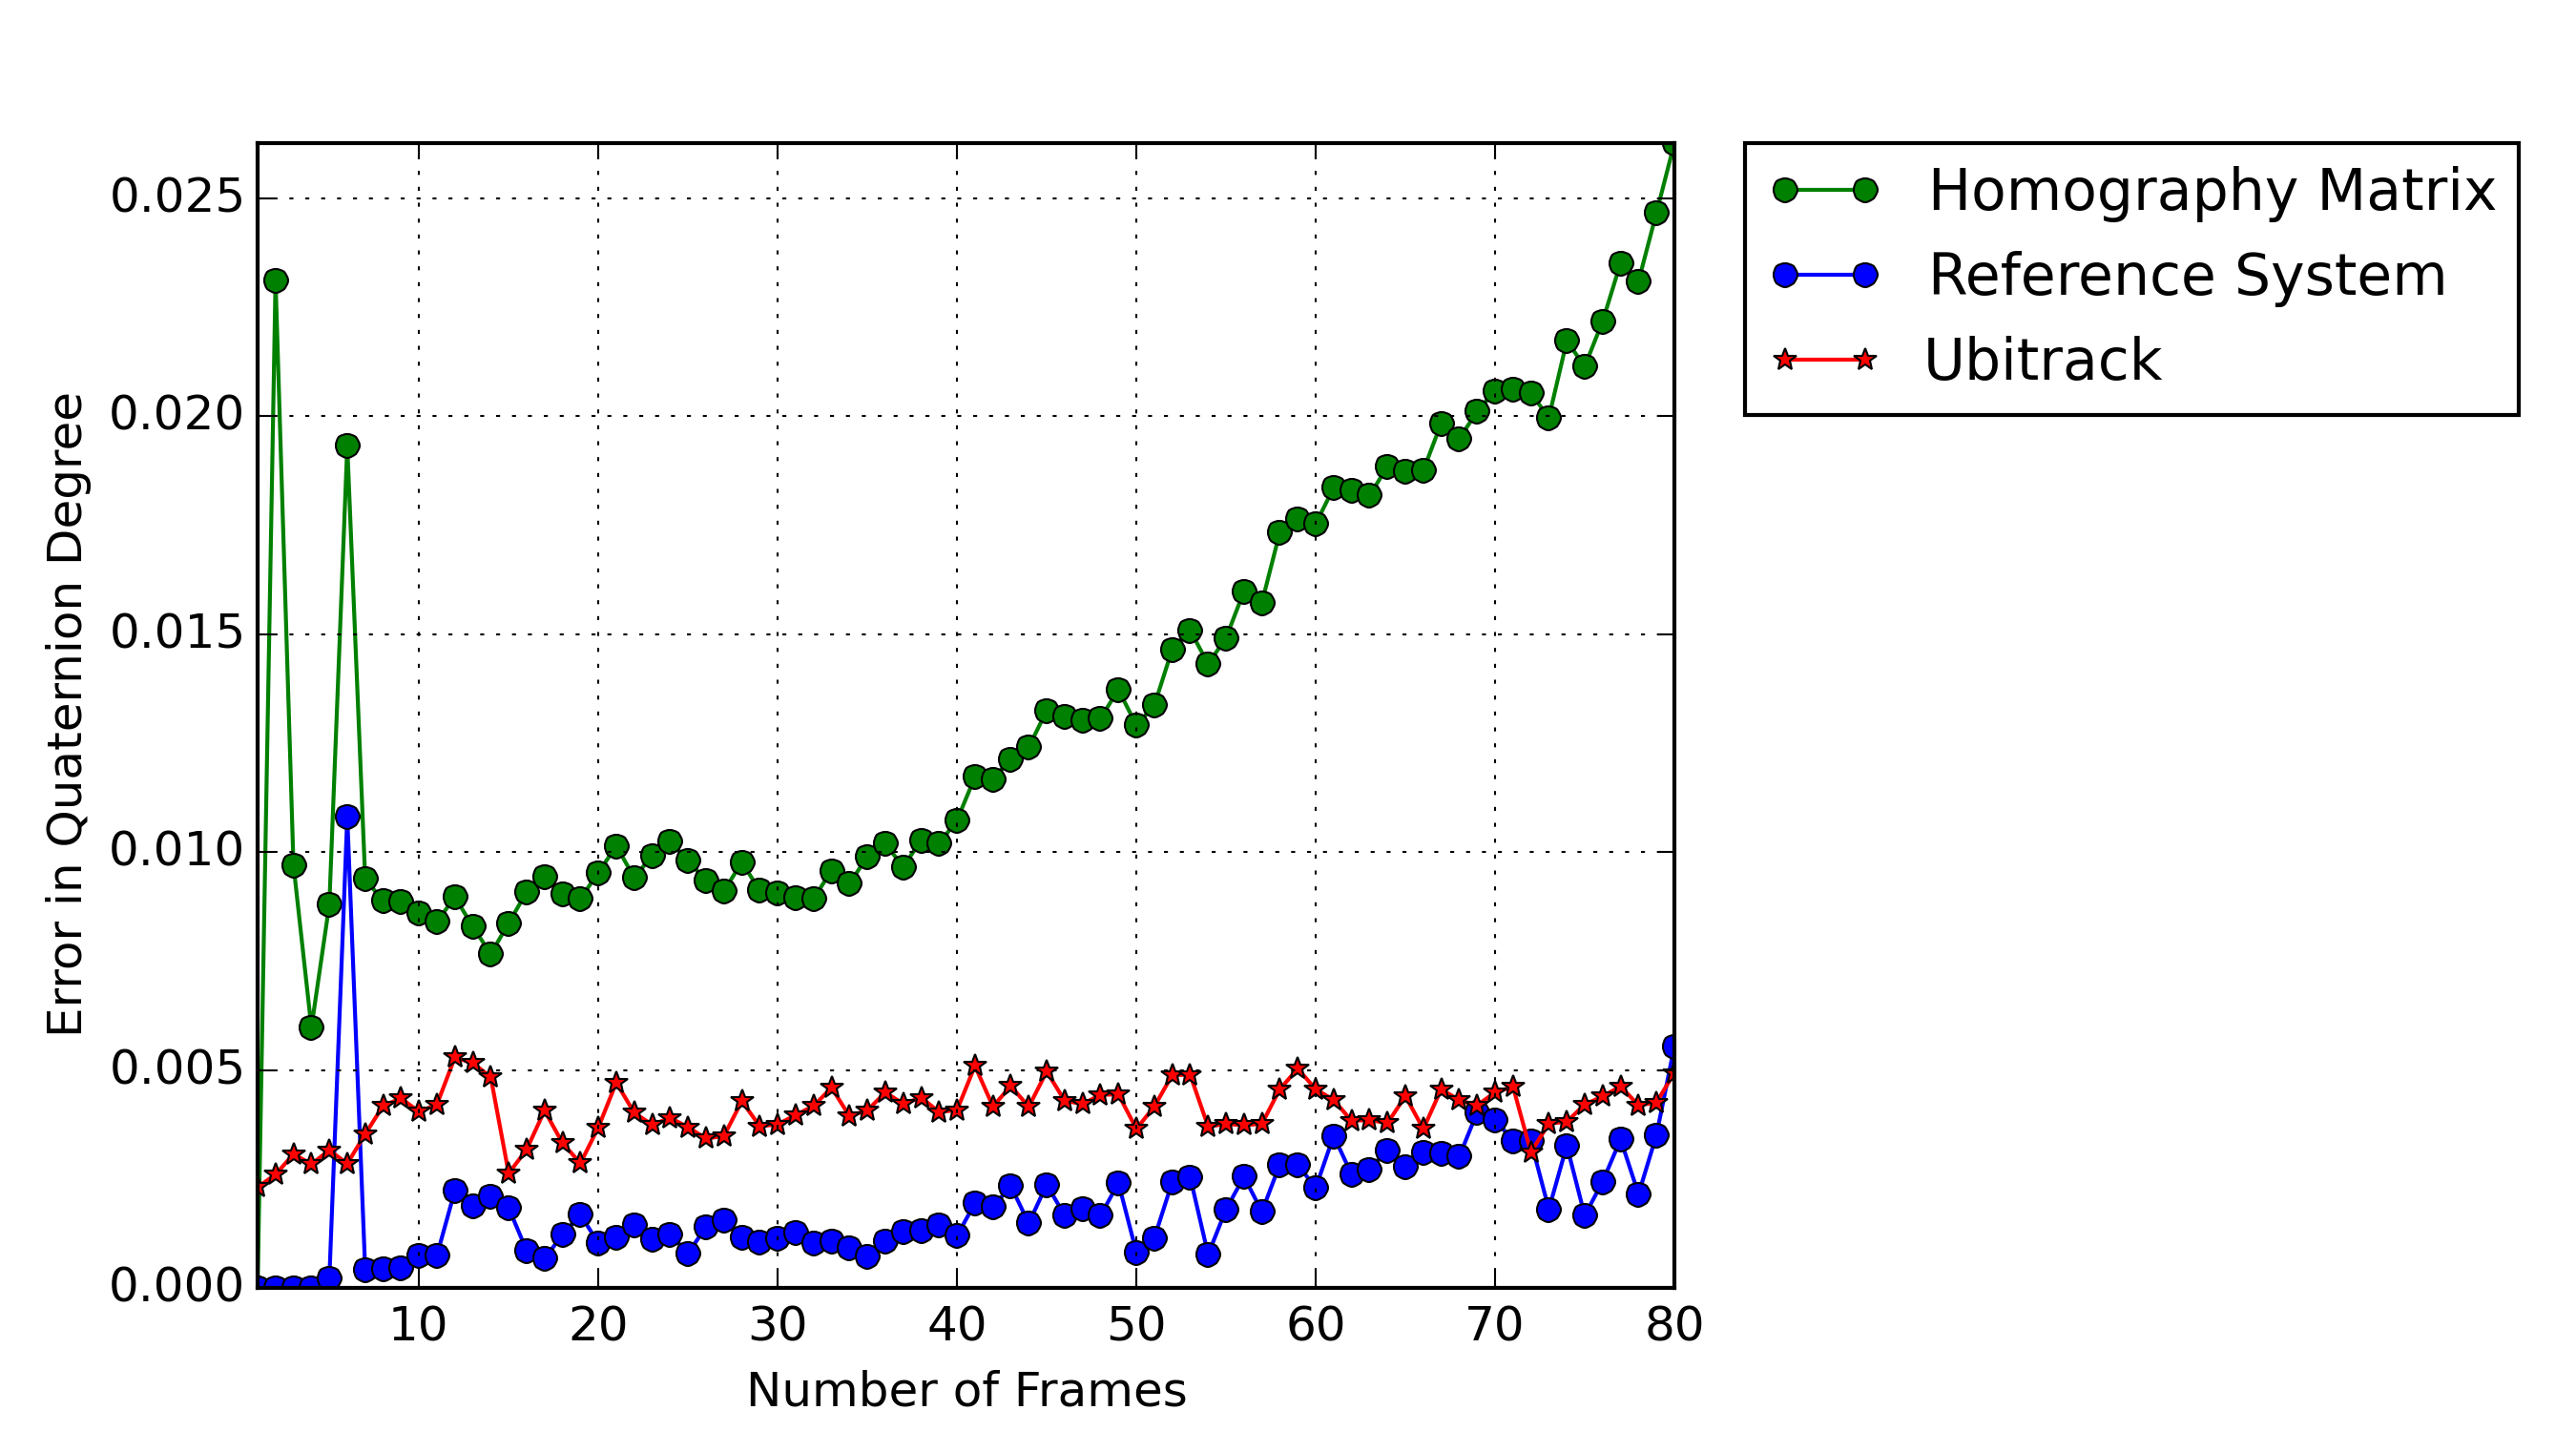
\includegraphics[width=80mm]{figures/homo/graph_rotation} \\
	(a) the translation error & (b) the rotation error \\[6pt]
\end{tabular}
\caption{The comparison of result of methods that use for computing the camera reference pose }\label{fig:diff_reference}
\end{figure}

\begin{table}[H]
\centering
  \begin{tabular}{| c || c | c | c | c |}
      \hline
      & \multicolumn{2}{c|}{Translation} & \multicolumn{2}{c|}{Rotation} \\ \hline
       & Mean & Standard Deviation & Mean & Standard Deviation \\ \hline
      Homography Matrix & 8.7867 & 5.9866 & 0.0135 & 0.0053 \\ \hline
      Reference System & \textbf{1.3303} & 1.1184 & \textbf{0.0019} & 0.0015 \\ \hline
      Marker-based Ubitrack & 10.1552 & \textbf{0.9700} & 0.0040 & \textbf{0.0006} \\ \hline
  \end{tabular}
  \caption{The statistical analysis of feature-based with ARTrack reference pose compare to the planner tracking reference pose} \label{tab:reference_system}
\end{table}

\section{Future Work}
In previous sections, the result of our feature-based pose estimation were testes and analyzed. In most of augmented reality applications and for small workspace, the tracking phase and estimating the movement of camera is more important than the rotation. The results of tests show that this approach in significantly robust and precise for all situation and geometric transformation. The drawback point of this technique that you can see in \autoref{fig:sample_02} and \autoref{tab:sample_02} is refereed to this fact that the result of estimated rotation in most of data sets are not efficient. To resolve this problem, it is better to investigate on the new algorithms in this case. Some new approaches were introduced in \autoref{sec:PnP_problem} that their results can improve our estimated rotation. \\
The other aspect that we can investigate on them is use the dynamic approach for the two local and global threshold. Our result show that the best value for the local and global threshold are 5 and 35 respectively. But sometimes due to lack of the number of the matches vector (for both 3D and 2D) it is better to instead of a fixed number for the local and global threshold, a dynamic mechanism is applied to set the size of these parameters. Simon Gibson and et. al in \cite{gibson2002accurate} introduced a dynamic solution for this purpose as follows:
\begin{itemize}
\item When the sequence reached to the end or 10 frames are processed
\item More than 50\% of the frames are lost. It means the size of matches vector between the $n$ and $n-1$ frames reached to less than the 50\% of matches vector between the first and second frames.
\end{itemize}